%% ----------------------------------------------------------------
%% Thesis.tex -- MAIN FILE (the one that you compile with LaTeX)
%% ---------------------------------------------------------------- 

% Set up the document
\documentclass[a4paper, 12pt, oneside]{Thesis}  % Use the "Thesis" style, based on the ECS Thesis style by Steve Gunn
\graphicspath{{Resources/Figures/MultiPurpose/}}  % Location of the graphics files (set up for graphics to be in PDF format)

% Include any extra LaTeX packages required
\usepackage[square, numbers, comma, sort&compress]{natbib}  % Use the "Natbib" style for the references in the Bibliography
\usepackage{verbatim}  % Needed for the "comment" environment to make LaTeX comments
% \usepackage{vector}  % Allows "\bvec{}" and "\buvec{}" for "blackboard" style bold vectors in maths
\usepackage{tabu}
\usepackage[usenames,dvipsnames]{xcolor}
\usepackage{colortbl}
\hypersetup{urlcolor=blue, colorlinks=true}  % Colours hyperlinks in blue, but this can be distracting if there are many links.
\hyphenation{ma-ker an-a-lyzed Baye-si-an pher-o-mone out-going}
\usepackage{algpseudocode}
\usepackage{algorithm}
\usepackage{xcolor}
\usepackage[lofdepth=1,lotdepth]{subfig}
\usepackage{grfext}
\PrependGraphicsExtensions*{.pdf,.PDF}
\numberwithin{algorithm}{chapter}  
\pdfminorversion=7
\usepackage{atbegshi}% http://ctan.org/pkg/atbegshi
\AtBeginDocument{\AtBeginShipoutNext{\AtBeginShipoutDiscard}}
\usepackage{IEEEtrantools}

\lstset{%
  numbers=none,
  tabsize=3,
  captionpos=b,
  breaklines=true,
  basicstyle=\small\ttfamily,
  framerule=0pt,
  backgroundcolor=\color{gray!25},
  keywordstyle=\color{blue},commentstyle=\color{darkgreen},stringstyle=\color{red},
  columns=fullflexible
}

%% ----------------------------------------------------------------
\begin{document}
%\bstctlcite{IEEEexample:BSTcontrol}

\setlength{\headheight}{27.5pt}\textsl{}
\frontmatter	  % Begin Roman style (i, ii, iii, iv...) page numbering

% Set up the Title Page
\title  {Self-Organizing Autonomic Computing Systems for Cloud Resource Management}
\authors  {\texorpdfstring
            {\href{mailto:bsolomon@ncct.uottawa.ca}{Bogdan Solomon}}
            {Bogdan Solomon}
            }
\addresses  {\groupname\\\deptname\\\univname}  % Do not change this here, instead these must be set in the "Thesis.cls" file, please look through it instead
\date       {November 2016}

\maketitle
%% ----------------------------------------------------------------

\setstretch{1.3}  % It is better to have smaller font and larger line spacing than the other way round

% Define the page headers using the FancyHdr package and set up for one-sided printing
\fancyhead{}  % Clears all page headers and footers
\rhead{\thepage}  % Sets the right side header to show the page number
\lhead{}  % Clears the left side page header

\pagestyle{fancy}  % Finally, use the "fancy" page style to implement the FancyHdr headers

%% ----------------------------------------------------------------
% The "Funny Quote Page"
\pagestyle{empty}  % No headers or footers for the following pages

\null\vfill
% Now comes the "Funny Quote", written in italics
\textit{``Blessed are those who find wisdom, those who gain understanding.''}

\begin{flushright}
Proverbs 13
\end{flushright}

\vfill\vfill\vfill\vfill\vfill\vfill\null
\clearpage  % Funny Quote page ended, start a new page
%% ----------------------------------------------------------------

% The Abstract Page
\addtotoc{Abstract}  % Add the "Abstract" page entry to the Contents
\abstract{
\addtocontents{toc}{\vspace{1em}}  % Add a gap in the Contents, for aesthetics

In recent years, a great deal of research has been undertaken in the area of automating the enterprise IT Infrastructure. For enterprises with a large number of computers, the IT Infrastructure represents a considerable amount of the enterprise budget assigned to its operation. Autonomic Computing Systems are systems which were created to correct and optimize the IT infrastructure's own self-functioning by executing corrective operations without any need for human intervention. Applications of autonomic systems range from usage optimization for clusters of servers or virtual machines, to error prevention and error recovery for web applications. In most cases where autonomic computing systems have been developed, this was achieved by the addition of external global controllers monitoring the subsystems of the enterprise IT Infrastructure, determining where changes should be made and applying appropriate commands to implement these changes. At the same time, the software industry has seen an explosion in the usage of cloud based services. By moving services in the cloud, companies can decrease the IT budget such that they only use the resources which are needed, when they are needed. Furthermore, services deployed in the cloud can be distributed geographically across multiple datacenters such that users obtain a higher quality of service by connecting to a closer datacenter. Self-Organizing systems are systems which reach a global desired state without the use of any central authority. Such systems are better suited to manage a cloud of servers than a centralized controller as they scale better when the controlled system is scaled also. In this thesis, an autonomic system based on a self-organizing architecture is introduced. The system is applied to the self-optimization of a web-based real-time collaborative application running on a geographically distributed cloud. Experiments and simulations with the self-organizing, self-optimizing autonomic computing methodology are given to support the design and the implementation described.

}

\clearpage  % Abstract ended, start a new page
%% ----------------------------------------------------------------

\setstretch{1.3}  % Reset the line-spacing to 1.3 for body text (if it has changed)

% The Acknowledgements page, for thanking everyone
\acknowledgements{
\addtocontents{toc}{\vspace{1em}}  % Add a gap in the Contents, for aesthetics

I would like to first thank my supervisor, Dr. Dan Ionescu, for the guidance and encouragement that I received during my Master's and PhD work as well as for the opportunity of doing this degree. At the same time, I would like to thank Dr. El Saddik for starting me, while I was still an undergraduate student, on the path that lead here.

Special thanks also go to all the people in the NCCTLab at University of Ottawa who allowed me to bounce ideas off of them and listened to my endless complaints.

I would also like to thank my parents and my brother for always cultivating in me the need to know more. 

Last but not least, special thanks go to my wife who pushed me and encouraged me to finish this thesis, and God who gave me the wisdom to complete it.

}
\clearpage  % End of the Acknowledgements
%% ----------------------------------------------------------------

\pagestyle{fancy}  %The page style headers have been "empty" all this time, now use the "fancy" headers as defined before to bring them back


%% ----------------------------------------------------------------
\lhead{\emph{Contents}}  % Set the left side page header to "Contents"
\tableofcontents  % Write out the Table of Contents

%% ----------------------------------------------------------------
\lhead{\emph{List of Figures}}  % Set the left side page header to "List if Figures"
\listoffigures  % Write out the List of Figures

%% ----------------------------------------------------------------
\lhead{\emph{List of Tables}}  % Set the left side page header to "List of Tables"
\listoftables  % Write out the List of Tables

%% ----------------------------------------------------------------
\setstretch{1.5}  % Set the line spacing to 1.5, this makes the following tables easier to read
\clearpage  % Start a new page
\lhead{\emph{Abbreviations}}  % Set the left side page header to "Abbreviations"
\listofsymbols{ll}  % Include a list of Abbreviations (a table of two columns)
{
% \textbf{Acronym} & \textbf{W}hat (it) \textbf{S}tands \textbf{F}or \\
\textbf{ACM}  & \textbf{A}ssociation for \textbf{C}omputing \textbf{M}achinery \\
\textbf{ARM} & \textbf{A}pplication \textbf{R}esponse \textbf{M}easurement \\
\textbf{CDN} & \textbf{C}ontent \textbf{D}elivery \textbf{N}etwork \\
\textbf{DMTF} & \textbf{D}istributed \textbf{M}anagement \textbf{T}ask \textbf{F}orce \\
\textbf{EC2} & \textbf{E}lastic \textbf{C}loud  \textbf{C}omputing \\
\textbf{EVO} & \textbf{E}nigmatec \textbf{V}irtual \textbf{O}rchestrator \\
\textbf{FCFS} & \textbf{F}irst \textbf{C}ome \textbf{F}irst \textbf{S}erved \\
\textbf{FEC} & \textbf{F}orward \textbf{E}rror \textbf{C}orrection \\
\textbf{GMS} & \textbf{G}roup \textbf{M}embership \textbf{S}ervice \\
\textbf{IEEE} & \textbf{I}nstitute of \textbf{E}lectrical and \textbf{E}lectronics \textbf{E}ngineers \\
\textbf{JEE} & \textbf{J}ava \textbf{E}nterprise \textbf{E}dition \\
\textbf{JMX} & \textbf{J}ava \textbf{M}anagement e\textbf{X}tension \\
\textbf{JSON} & \textbf{J}ava\textbf{S}cript \textbf{O}bject \textbf{N}otation \\
\textbf{MAPE} & \textbf{M}onitor \textbf{A}nalyze \textbf{P}lan \textbf{E}xecute \\
\textbf{N1 SPS}  & \textbf{N1} \textbf{S}ervice  \textbf{P}rovisioning \textbf{S}ystem \\
\textbf{QNM} & \textbf{Q}ueueing \textbf{N}etwork  \textbf{M}odel \\
\textbf{QoS} & \textbf{Q}uality \textbf{o}f \textbf{S}ervice \\
\textbf{SLA} & \textbf{S}ervice \textbf{L}evel \textbf{A}greement \\
\textbf{SOAP} & \textbf{S}imple \textbf{O}bject \textbf{A}ccess \textbf{P}rotocol \\
}

%% ----------------------------------------------------------------
%\clearpage  % Start a new page
%\lhead{\emph{Physical Constants}}  % Set the left side page header to "Physical Constants"
%\listofconstants{lrcl}  % Include a list of Physical Constants (a four column table)
%{
% Constant Name & Symbol & = & Constant Value (with units) \\
%Speed of Light & $c$ & $=$ & $2.997\ 924\ 58\times10^{8}\ \mbox{ms}^{-\mbox{s}}$ (exact)\\

%}

%% ----------------------------------------------------------------
%\clearpage  %Start a new page
%\lhead{\emph{Symbols}}  % Set the left side page header to "Symbols"
%\listofnomenclature{lll}  % Include a list of Symbols (a three column table)
%{
% symbol & name & unit \\
%$a$ & distance & m \\
%$P$ & power & W (Js$^{-1}$) \\
%& & \\ % Gap to separate the Roman symbols from the Greek
%$\omega$ & angular frequency & rads$^{-1}$ \\
%}
%% ----------------------------------------------------------------
% End of the pre-able, contents and lists of things
% Begin the Dedication page

\setstretch{1.3}  % Return the line spacing back to 1.3

\pagestyle{empty}  % Page style needs to be empty for this page
\dedicatory{Dedicated to my wife, my parents and my brother}


\addtocontents{toc}{\protect\setcounter{tocdepth}{2}\vspace{2em}}  % Add a gap in the Contents, for aesthetics


%% ----------------------------------------------------------------
\mainmatter	  % Begin normal, numeric (1,2,3...) page numbering
\pagestyle{fancy}  % Return the page headers back to the "fancy" style

% Include the chapters of the thesis, as separate files
% Just uncomment the lines as you write the chapters

% Chapter 1

\chapter{Introduction} % Write in your own chapter title
\label{Chapter_introduction}
\lhead{Chapter \ref{Chapter_introduction}. \emph{Introduction}} % Write in your own chapter title to set the page header

\section{Motivation and Research Objectives}

As IT departments have become more pervasive and more important for each and every company, as well as to our daily lives, they have also become more complex. In today's world people obtain their news and alerts online, shop online as well as communicate with friends and family via social networking sites. The complexity of the IT infrastructure has lead however to a situation where it is nearly impossible for humans to continue to manage and maintain the IT resources in a good state. Failures of the IT infrastructure in a company can have disastrous consequences for the company or even for the economy. In a world that is as fast as the current one an IT failure can result in lost sales, loss of customers to competitors or even payment of damages depending on how critical the infrastructure is.

Cloud computing exacerbates these issues by moving the IT infrastructure outside a company's premises. Where before each small enterprise would run its own small IT department, now large data centers provide IT services to multiple consumers and enterprises (SaaS, HaaS, IaaS). For the cloud providers, the ability to maintain the systems' service level agreements and prevent service outages is paramount since long period of failures can open them to large liabilities from their customers. At the same time, cloud computing provides the ability for companies to pay only for the required resources and to scale up or down as more resources are needed or as resources are no longer required. Due to this capability, a solution is needed for cloud computing users in order to intelligently decide when to request more servers and when to release used servers. From the point of view of cloud computing providers, a solution is needed in order to move server loads such that only the required resources are used for a certain demand via virtualization. Server virtualization also increases the complexity of managing the servers in data centers, since suddenly one single hardware server can be running tens of virtual machines, each with its own load and processing requirements. Ensuring that the appropriate number of virtual machines are deployed on a hardware platform, such that the hardware is neither underutilized, nor that the virtual machines starve each other for resources, is not a trivial administrative task. The issue becomes even more complex when the end user's location is taken into consideration. In order to achieve better response times and latency, it is preferable to offer services as close as possible to the end user. Such approaches can be seen in Content Delivery Networks (CDNs) \cite{akamai}, which cache web data in datacenters across the world in order to be closer to the end users. A similar approach is taken by Netflix in order to cache the most viewed shows and movies closer to the customers.

These are the problems that autonomic management systems attempt to solve. Autonomic computing systems are capable of self-managing by self-configuring, self-healing, self-optimizing and self-protecting, together known as self-CHOP. Such a system must be able to analyze itself at run time, determine its state, determine a desired state and then if necessary attempt to reach the desired state from the current state. Normally the desired state is a state that maintains the system's Service Level Agreement (SLA). For a self-configuring system for example, this could include finding missing libraries and installing them with no human intervention. A self-healing system would be able to determine errors in execution and recover to a known safe state. A self-optimizing system example would be a cluster of servers that dynamically adds and removes servers at run time in order to maintain a certain utilization and client response time. Finally, a self-protecting system example would be a server that detects a denial of service (DoS) attack and prevents it by refusing requests from certain Internet Protocol (IP) addresses.

The above goals of autonomic computing were mapped in the Manifesto \cite{IBM:AutonomicManifesto} containing eight key requirements that a system must meet to be considered autonomic. An autonomic computing system must:

\begin{enumerate}
	\item ``Know itself'' by knowing its components, status, ultimate capacity, and other interconnected systems
	\item Configure and reconfigure itself under various and sometimes unpredictable situations. The configuration must be done automatically by the system
	\item Never settle for the status quo, and must always try to optimize the available resources, itself, and the way it works
	\item Be able to heal itself in case of malfunctions on some of its parts, and be able to recover its normal state of execution
	\item Be able to protect itself by identifying and responding to threats against various types of attacks, while maintaining system integrity and security
	\item Be aware of its environment and act according to the environmental needs
	\item Function in a heterogeneous and open way, and implement open standards
	\item Keep its complexity hidden from the end user
\end{enumerate}

Since the release of the Manifesto, a number of research directions and a corresponding number of projects have been developed to look at how to create such intelligent systems which can substitute human intervention with automatically generated operative commands. Various approaches have been taken to reach the desired system self-adaptation qualities. In terms of how the self-management behavior is reached two main architecture approaches have been used. In the first approach, a global controller is added to the system, which gathers data from the various components, performs some form of analysis on the data, and compares the analysis results with the desired goals. If the goals are breached by the predicted analysis, corrective actions are taken. Such approaches are seen in \cite{related:architecture:hierarch1}, \cite{related:model:lqm} and \cite{bogdan:seams07}. In the first type of approaches, a cluster of servers would (for example) have one controller which manages the entire cluster's adaptation. The second approach attempts to develop an autonomic system by developing small intelligent subsystems which achieve global self-adaptation through the interactions with other components. Such approaches can be seen in \cite{related:architecture:selflet} and \cite{related:architecture:unity}. In this second approach, each server in a cluster would have its own intelligence which achieves local adaptation. The communication between components is then used in order to reach global system adaptation. Such systems can be developed by looking at Self-Organizing systems, which are systems that are capable of reaching a desired state without the use of any central authority or plan. This type of system can be seen in Ashby's homeostat \cite{ashby:homeostat} which is capable of adapting itself to any perturbation in the system and reach back a stable state. Self-Organizing Networks have also been developed in recent years for mobile networks.

In this thesis, a \textbf{Self-Organizing autonomic system} which self-manages a cloud of servers is introduced. The system architecture, system design and results obtained via simulations and experiments with a live system are presented. The self-managing function ensures that all the servers in the same data-center maintain the same response time and CPU usage. At the same time, the self-organizing system can add or remove servers as needed when load for the service increases or decreases.

The motivation for developing an autonomic computing system to manage the cloud deployment is related to providing intelligent scaling of the cloud resources such that only the required resources are used at a given point in time. With the autonomic system managing the cloud resources, it can be ensured that servers are not idle when users do not need them. At the same time when demand increases the autonomic system ensures that more servers are started such that the latency and response time of the system are maintained at desired levels.

\section{Organization of the Thesis and Research Focus}

The thesis is organized such that it presents the self-organizing autonomic system moving from the design of the autonomic control system to various mechanisms which have to be set up to ensure the self-optimization of the cloud resources usage. Simulation results as well as results from a live system are also shown. The rest of the thesis comprises the following.

Chapter \ref{Chapter_related} presents the goals of the self-organizing system and also presents various related work in both autonomic architectures and self-organizing problems.

Chapter \ref{Chapter_selfopt} describes the self-organization approach for the self-optimizing control of cloud resources. In this case self-optimization refers to providing automatic elasticity for the cloud. The self-optimizing system is split into two algorithms. The first algorithm is responsible for predicting SLA breaches and the second algorithm optimizes the size of the cloud when faced with SLA breaches.

Chapter \ref{Chapter_testbed} presents a cloud simulation environment used to compare the proposed system with other auto-scaling systems as well as a test bed running a collaborative application.

Chapter \ref{Chapter_results} shows the performance tests for the self-organizing self-optimizing system which were obtained in the simulation environment and on the test bed.

Finally chapter \ref{Chapter_conclusions} presents conclusions of the benefits provided by the proposed solution. Future developments of the architecture are also described.

The thesis' research focus will be on a number of contributions to the field of autonomic computing and self-organizing systems, as presented in \cite{bogdan:lindi}, \cite{bogdan:amgcc2013}, \cite{bogdan:cts2012}, \cite{bogdan:conti2010}, \cite{bogdan:saci2013} and \cite{bogdan:miles2012chapter}. 

The research will focus on a new self-organizing approach used for server scaling in data-centers and cloud systems which will allow heterogeneous resources to be part of the same server cloud, while normally a self scaling system will use homogeneous only resources. The designed self-organizing self-optimizing system will be split in two parts: a self-organizing system responsible for predicting breaches of the cloud's SLA and a second self-organizing algorithm which optimizes the number of servers used in the cloud when a breach is detected.

A simulation environment and test-bed are used in order to obtain results on the performance of the self-organizing autonomic system while managing various types of cloud resources - showing the versatility of the proposed approach. % Introduction

\chapter{Autonomic and Self-Organizing Systems: A Review} % Write in your own chapter title
\label{Chapter_related}
\lhead{Chapter \ref{Chapter_related}. \emph{Autonomic and Self-Organizing Systems: A Review}} % Write in your own chapter title to set the page header

This chapter presents the known approaches for autonomic computing and self-organizing systems and motivates the need for developing a self-organizing architecture for the autonomic management of cloud resources, including the advantages that such an architecture would provide. The chapter also introduces prior work in the area of simulation systems for clouds and provides motivation why the simulation framework used in this thesis was selected.

\section{Reasons for Self-organizing Architecture}

Since the introduction of autonomic systems by IBM \cite{IBM:acblueprint}, autonomic systems have been developed using the Monitor, Analyze, Plan, Execute (MAPE) loop. Figure \ref{fig:MAPELoop-IBM} shows the loop as described by IBM. The resource under control, which can be as simple as a single server or as complex as a cluster of servers, is constantly being monitored to determine changes in its state. This monitoring can be either periodic measurements of certain values in the system, like CPU utilization or response time, or alarm-based when certain conditions are breached and an alarm is raised. Once the measured or alarm data is obtained by the monitor function, the data is passed on to the analyze function which uses its internal logic and rules in order to analyze the data and to determine if the system is exhibiting any problems. If a problem is discovered, the problem information is sent to the plan function whose role is to determine an appropriate response to fix the existing problem or problems. The plan function creates an execution plan which will fix the problem and bring the controlled resource back into compliance. The execution plan is then delivered to the execution function which puts the plan into execution by making modifications to the resource and to the resource's environment.

\begin{figure}
	\centering
		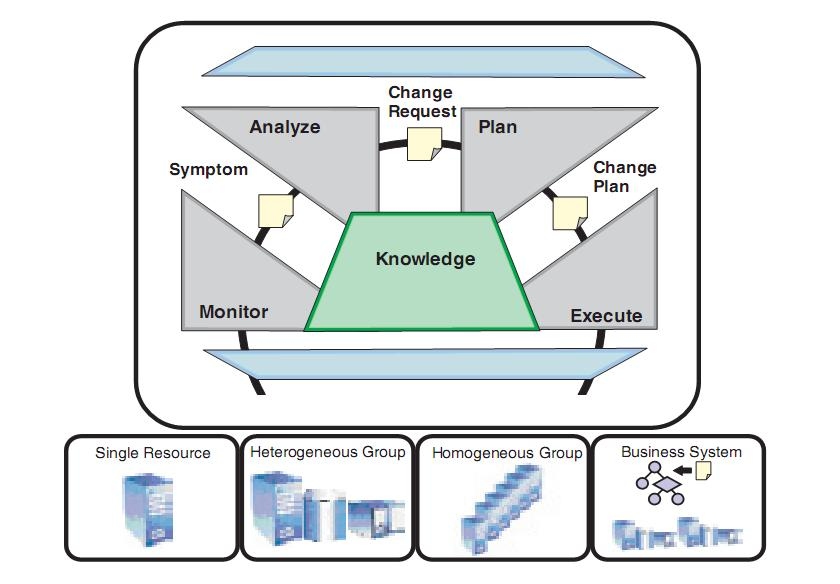
\includegraphics[width=14.6 cm]{MAPELoop-IBM.jpg}
		\caption{MAPE Loop}
	\label{fig:MAPELoop-IBM}
\end{figure}

In order to illustrate the autonomic system approach, consider a cloud of servers. The goal of the autonomic system is to maintain a good utilization of the server resources, while at the same time guaranteeing a certain level for the cloud's response time. For such a case, the autonomic control loop would measure all the servers' response times and CPU usage. If the response time becomes too high, as determined by the analyze function, the plan function calculates how many new servers to add to the cloud. Once the number of new servers is determined, the execute function is responsible for bringing those servers online by starting them and adding them to the cloud. If the CPU usage of the servers in the cloud decreases too much however, the plan function calculates how many servers to remove from the cloud. It is then the responsibility of the execute function to stop the correct servers, remove them from the cloud and free any other resources used by the servers.

Two main approaches have been taken in research in order to build autonomic systems. These approaches are presented in more detail in the following sections. The first approach considers the entire system under control as a single unit and attempts to add a global control loop which controls the entire system. In the above example, such a system would gather data from all the servers and use some form of mathematical approach like an averaging of the measured data in order to estimate the state of the entire cloud. Based on this average, the system would then determine any breach of Service Level Agreement (SLA) and create a plan if a breach exists. This approach has a number of assumptions on how the cloud is formed and how the cloud behaves. First of all, the autonomic control system assumes all the servers in the cloud are exactly the same. If the cloud was heterogeneous, then it would not be possible to average the measured data to obtain a global view of the cloud - unless a more complex procedure is used where the analyze function also knows ahead of the time the relative power of all the servers. Second of all, the system not only assumes that all servers are the same, but also behave the same, and, in addition, that client requests are balanced appropriately across all servers. If this was not the case, it would be possible to have, for example, two types of requests A and B, where A type requests are much more computationally intensive than B, and where all the A requests go to Server 1 and B requests to Server 2. Such a case could lead to an undesirable situation where the response time of Server 1 is above the desired SLA, but the average between Server 1 and Server 2 is below the desired SLA.

The second approach views the system under control as a composition of smaller subsystems (servers in the example given above) which are to be controlled. Through the control of each of these subsystems, a desired global SLA level can be reached. In the above example, each of the servers would have its own control loop responsible only for that server and which is ensuring that the server maintains a response time bellow the required SLA. Such an approach allows for heterogeneous resources to be part of the same cloud. It also allows for mixed clouds which can contain virtualized and non-virtualized servers running together. Furthermore, requests do not need to be balanced across servers; as long as each server correctly maintains its own SLA, even if the cloud encounters a case similar to the previous example where all request of type A come to one server and all requests of type B reach another server, the system will maintain a good SLA across all servers in the cloud. An extra advantage of this approach is that it scales very well even with a very high number of subcomponents (servers). For the centralized approach, if the number of servers increases too much, the central controller starts exhibiting load and latency issues as well. With a decentralized approach, the cloud can theoretically grow forever without suffering degradation due to the control plane. The problem with decentralized systems is that they are more complicated to design, deploy and manage.

There are other approaches used in literature which are somewhere between a fully centralized and a fully decentralized approach. For example, hierarchical controllers may have subcontrollers that take local decisions under the supervision of a parent controller. Such systems will exhibit some of the drawbacks of fully centralized systems but without all the design and deployment problems of fully centralized systems.

One approach which matches well to decentralized systems is the approach of Self-organizing systems, as Self-organizing systems are systems in which a desired state is reached without the use of any central authority or plan. Self-organizing Systems can achieve high-level goals via the interaction and communication between the components and without the need for a global controller which manages each and all of the subcomponents of the system. From these interactions and communications an emergent system appears which can exhibit self-optimizing features as required by autonomic computing. This approach is the one taken in this thesis due to the advantages that it offers compared to a global controller.

\section{Related Work}

Autonomic computing has become a very important field in research and industry due to the complexity of the IT infrastructure. Autonomic computing is also one of the fundamental technologies required for cloud computing and management of virtualized resources. All autonomic research is based on the MAPE loop in one form or another. This, however, did not prevent a diversity of approaches to be taken. Multiple architectures have been proposed, as well as various control techniques from machine learning to control theory. This section will be composed of related work in autonomic system architectures, various approaches for the MAPE loop components, self-organizing systems, as well as in real-time collaborative systems.

\subsection{Autonomic System Architectures}

All autonomic system architectures are based on the initial proposal of the MAPE loop made by IBM, also sometimes known as a MAPE-K loop to include the knowledge portion of the system. However, the use of the MAPE-K loop as a starting point did not hinder a variety of architectures from being proposed in research. The autonomic system architectures which can be found in literature can be split into three main types: decentralized architectures, hierarchical architectures and centralized architectures.

\subsubsection{Centralized Architectures}

Centralized architectures have a common characteristic in that the entire autonomic system - excluding sensors which can run on the measured entity - is running on a single machine which is responsible for running the entire MAPE-K loop and managing all the required resources. Such an approach can be found in the work done at Montana State University \cite{related:architecture:autonomicelement} where the autonomic architecture is developed as an Autonomic Element. The autonomic element is seen in this paper as the base building block for an autonomic system. An autonomic element is composed of two parts: the manager and the managed element. In their paper, the manager is described as a multi-threaded daemon, with each of the four MAPE functions, as well as the effectors and sensors, running in their own threads. Message passing is done via queues and synchronization is obtained via semaphores. Figure \ref{fig:centralizedarchi} shows a typical centralized architecture for three servers. All server data is measured by one controller, which performs the MAPE process and then takes control actions on the servers.

\begin{figure}
	\centering
		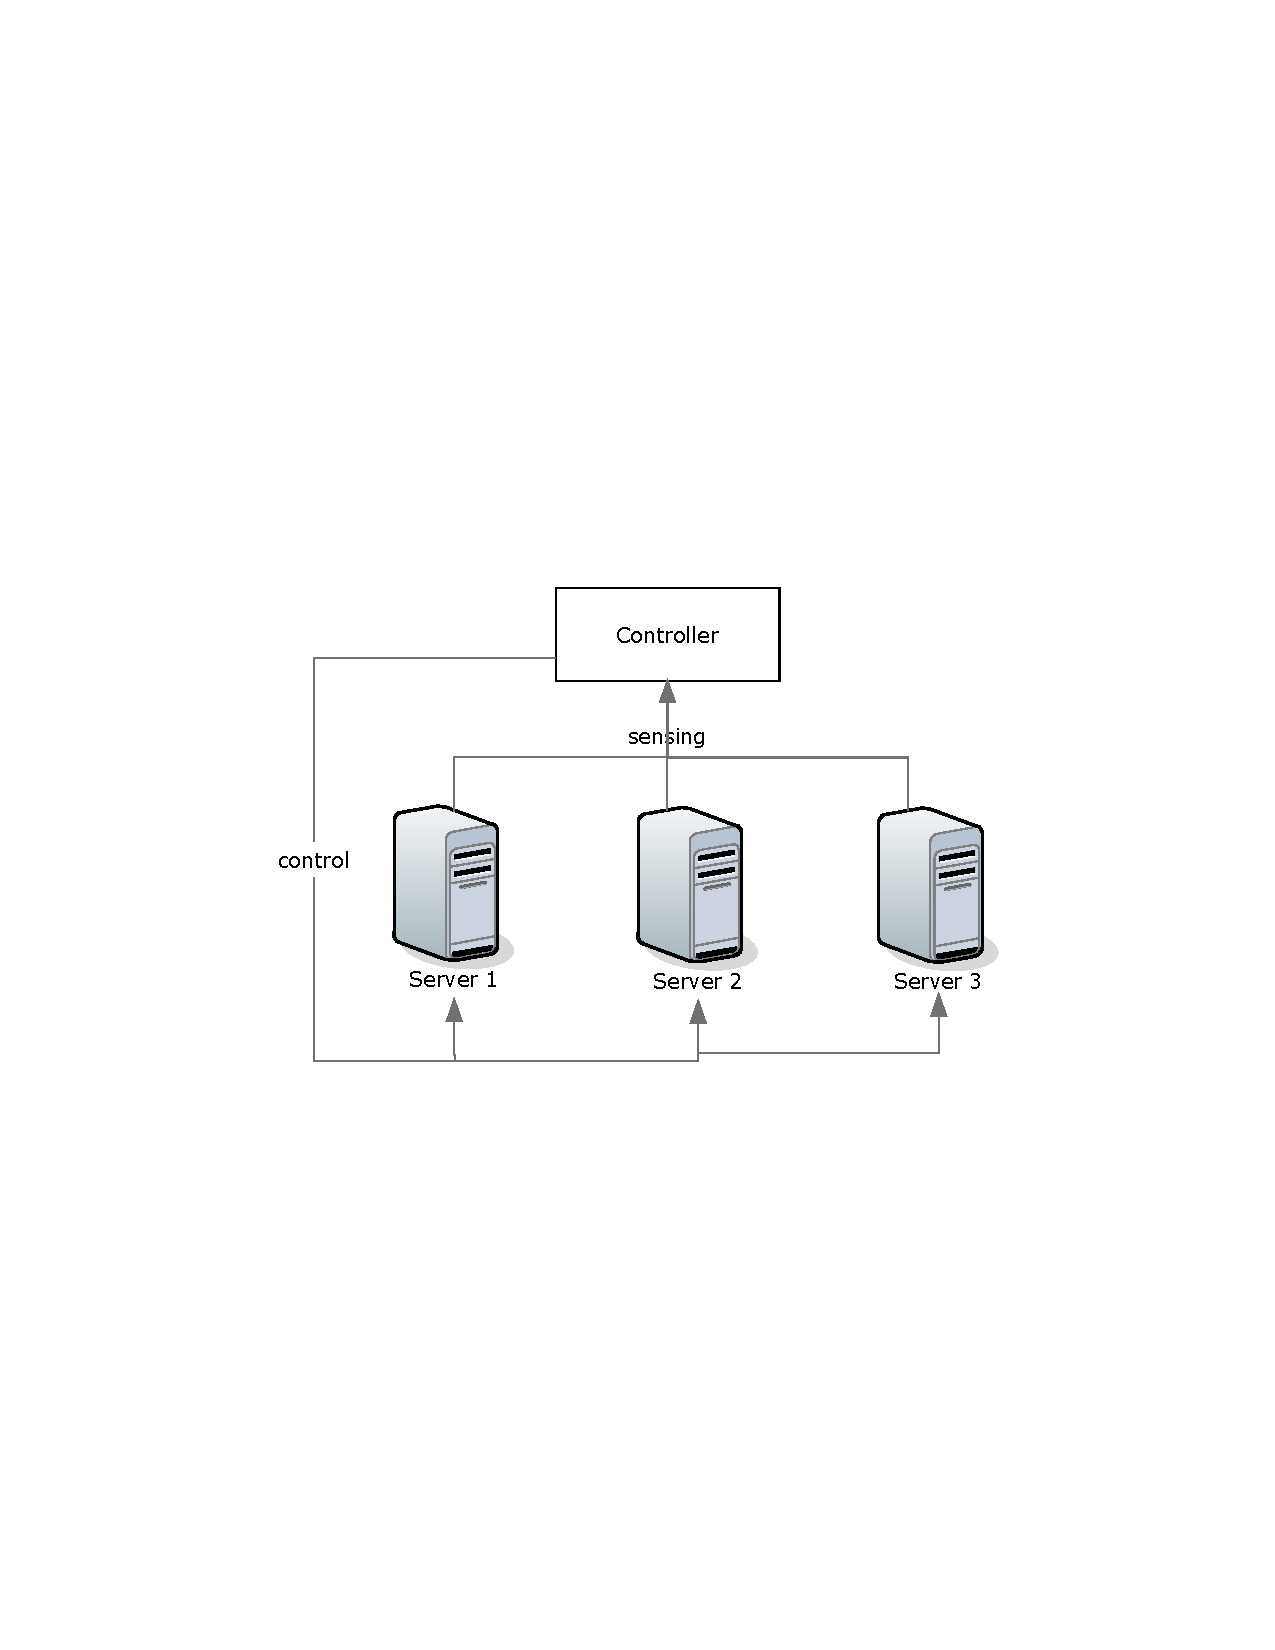
\includegraphics[width=0.75\linewidth]{ThesisRelatedArchiCentralized}
	\caption{Centralized Autonomic System Architecture}
	\label{fig:centralizedarchi}
\end{figure}

The architecture uses sensors to obtain data about the managed element and the environment, and defines two separate sensors for each autonomic element - one for internal data from the managed element and an external one for data from the environment. Similarly there are two effectors: one which passes required changes to the external environment and one which modifies the managed element internally. Furthermore, the architecture defines a ``data atom'' as the basic message that is passed throughout the system. Each atom is an XML data structure that contains version, priority, type and meta-data as well as the base data for the event. Furthermore, multiple atoms can be chained together to form a single atom if required by some common relation.

Since the architecture for an autonomic element uses separate threads for processing, care must be taken to ensure that the system performs correctly asynchronously and that there are no deadlocks in the system. In order to ensure the above, the authors of \cite{related:architecture:autonomicelement} propose the use of a priority queue for message passing. As data atoms are sent from one component to another, the atoms are stored in a queue based on their given priorities. The components then pop the respective atoms, process them, and either send them forward to the next component, create new atoms to be sent, or send the atoms to an empty data sink to be destroyed. In order to prevent deadlocks and starvation, the authors also use an extra object named a ``locker'', which is similar to a semaphore. A locker is placed between each two adjacent components and its role is to pass atoms between components. A locker receives an atom from a sending component, and notifies the receiving component that it has a new atom available for processing. Since polling is not used, it prevents synchronization and deadlock issues. Lockers are unidirectional, making it impossible to send data back to a previous component for processing, thus resulting in a sequential processing of data. In order to provide rapid response for sensors and effectors, the architecture uses data streams, which are one-way communication channels where one component writes data, and another reads the data in an atomic way. The system also uses a repository to store both processed atoms that are needed later, as well as policy rules. This repository acts as the knowledge base in the MAPE loop.

The above architecture has a number of problems which make it hard to use in most cases. First of all, the autonomic element architecture executes its entire process on a single machine. This causes problems, which apply to all centralized approaches, in cases where the managed element is a large structure, like a cloud, formed from hundreds of resources. A centralized approach will scale poorly as the number of resources which are monitored and managed increases. Furthermore, in the case of geographically distributed resources, the sensor data from the managed resources would have to travel through the internet to the manager, which can add large delays to processing the data and taking corrective actions. Finally, the architecture forces an autonomic element to have two sensors - one external and one internal, as well as two effectors. However there are cases were data comes from a varied number of sources, possibly each with its own data sample period, and where splitting the data inputs into more than two sensors is desired. Because of the above factors, the autonomic element architecture is restrictive in terms of the kind of autonomic system which can be developed and deployed.

Centralized architectures are also used by some systems developed in industry like IBM's Tivoli Intelligent Orchestrator (TIO) \cite{product:tio} and Sun N1 Service Provisioning System (SPS) \cite{product:n1}. TIO is capable of analyzing the CPU utilization of servers in a cluster and based on utilization over time, along with future predictions, decide if servers must be added or removed. Once a decision is reached, TIO deploys additional servers by finding available servers and, based on predefined workflows, provisions those servers and adds them to the cluster. A number of issues exist with the TIO platform. First of all, TIO assumes that all the servers in a cluster or resource pool are homogeneous in hardware and have the same behavior. This is rarely the case in data centers and even more so in clouds, where the deployment location could vary. Furthermore, even two computers with the same software/hardware will exhibit slightly different behavior. Second of all, TIO can not monitor multiple metrics, and provide multiple provisioning decisions to the same cluster. Only the CPU is monitored and only add/remove server actions are supported in the autonomic mode. Third of all, TIO is designed as a monolithic piece of software, making it hard to extend in order to add extra intelligent behavior. Unlike TIO which manages clusters of servers, N1 automates the deployment and configuration of web applications, thus providing the self-configuration characteristic of autonomic computing. Similarly to TIO, SPS is capable of provisioning operating system clones and applications in order to quickly configure a new server.

\subsubsection{Hierarchical Architectures}

Hierarchical architectures improve on centralized architectures by using multiple MAPE-K loops which are organized in a pyramid, with the low level control loops managing fine grained resources, while the high level control loops are responsible for the state of the entire system. Figure \ref{fig:hierarchicalarchi} shows a typical two-layer hierarchical architecture for three servers. Each of the servers has its own control loop and all the low-level control loops have a second layer which manages their parameters.

In \cite{Kramer:hierarch}, the authors propose a three layer architecture formed from bottom to top from: component control, change management and goal management. At the lowest level, the component control layer is concerned with short time scale operations and its goal is to modify the operating parameters of the component under management. At the change management level the system responds to changes in state reported from the lower level. This layer is reactive in that in response to a change in the lower level, it creates a plan to improve or maintain the execution of the system. This layer can, for example, add new components or modify existing components to maintain SLAs. Finally, the goal management layer is responsible for long timescale operations. It takes the state of the system and long ranging goals and produces plans which reach those goals. For example, this layer would be responsible to find available servers which should be deployed in order to maintain a required SLA, or how to migrate servers to maintain a desired redundancy rate after a server's failure. It should be noted that the author's architecture is based on Gat's model for robot architectures \cite{gat:robots}. 

\begin{figure}
	\centering
		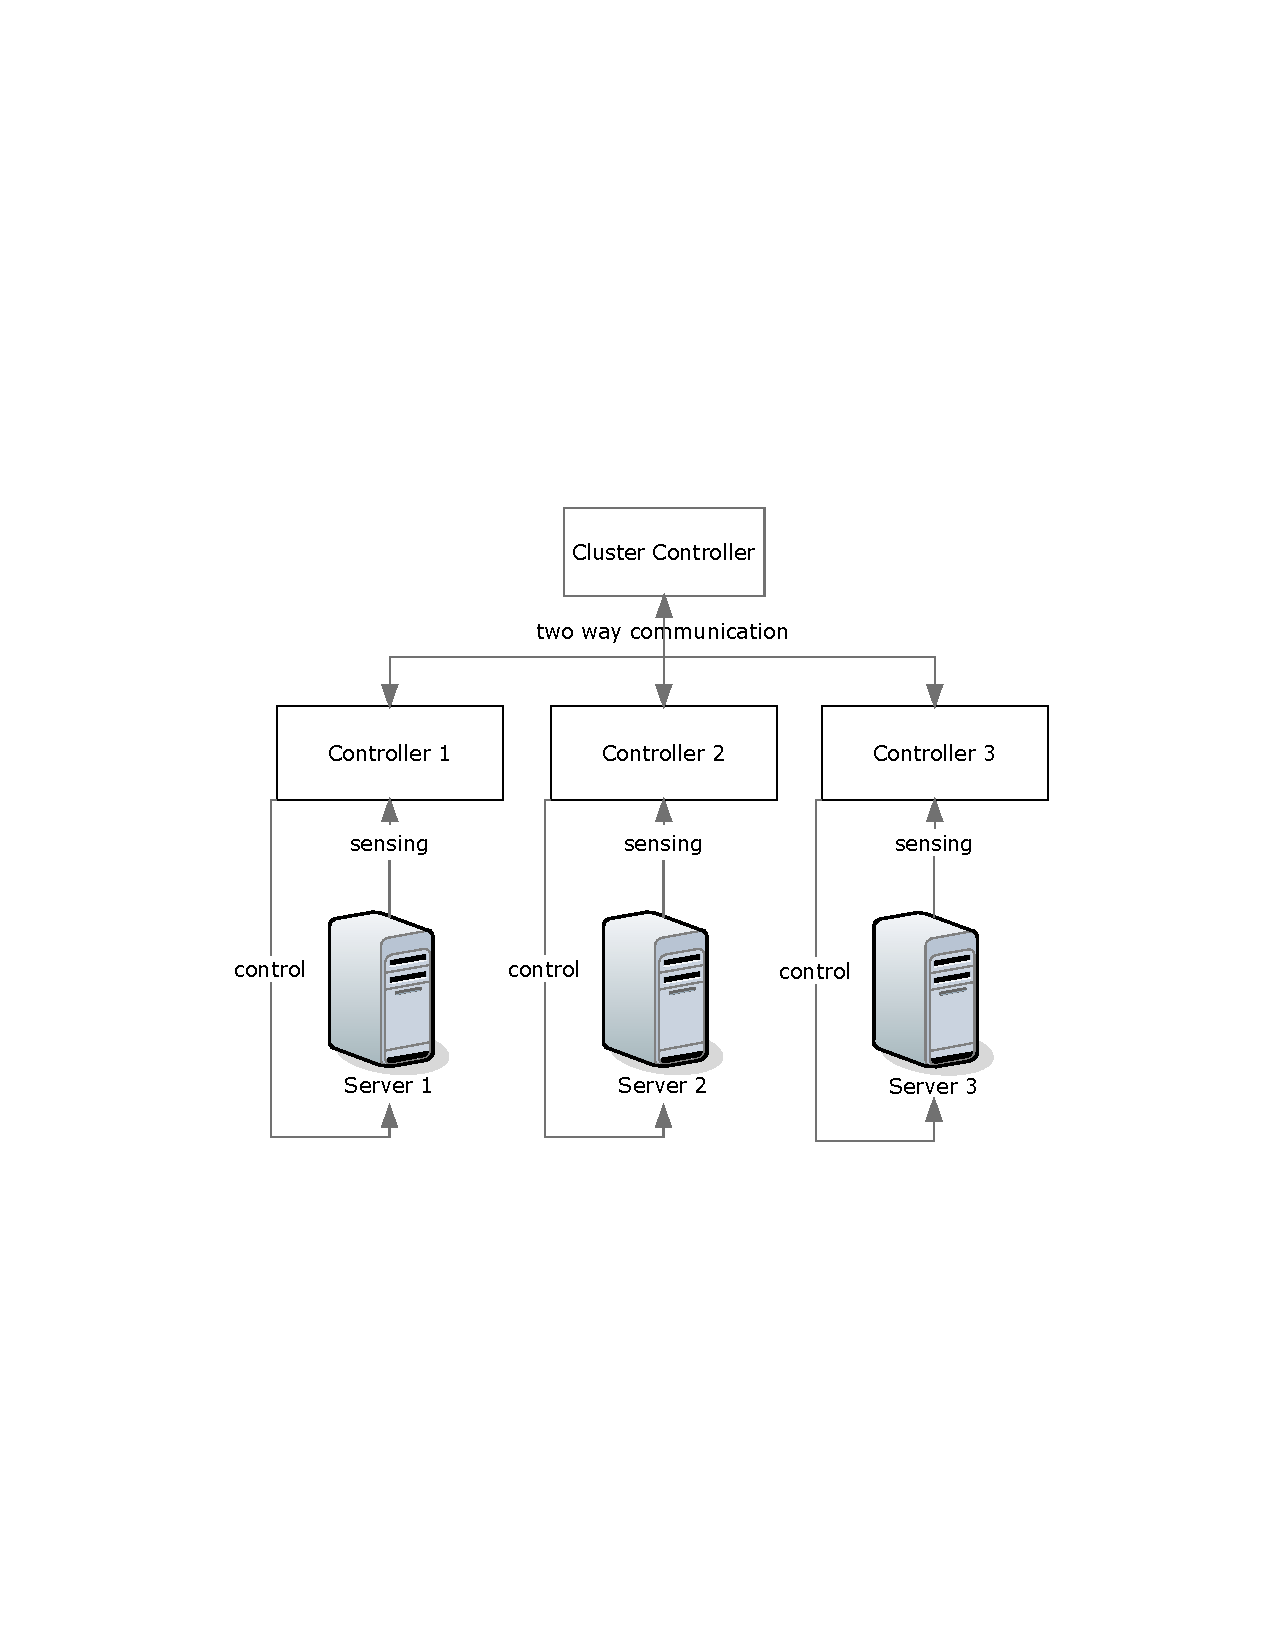
\includegraphics[width=0.75\linewidth]{ThesisRelatedArchiHierarch}
	\caption{Hierarchical Autonomic System Architecture}
	\label{fig:hierarchicalarchi}
\end{figure}

Similarly, in \cite{related:architecture:hierarch2}, the authors develop a three layer architecture where the system manages from bottom to top: the component, the application and the system. Similarly to the work in \cite{Kramer:hierarch} the component level manages a single component and takes actions that span a short time. This could be for example a web server which modifies its buffer pool size or thread pool size. By itself, this is not sufficient to manage the SLA of the system and the component level also can not set its own QoS targets. The middle level controller which is the application controller, manages the performance of the entire system by setting QoS parameters for the lower level controllers and taking over when the low level controllers can not reach the required QoS. Such an action could be to redistribute incoming requests to ensure that some servers are not overloaded. The highest layer controller - the provisioning controller - is responsible for rearranging the system when it can not meet its QoS without structural changes. Such changes can include adding or removing servers to/from the cluster in order to maintain the QoS attributes while also ensuring optimal utilization of resources.

While hierarchical architectures improve on centralized architectures by separating the control concern into multiple levels, where long running self-managing decisions can run at a higher level, while short timeframe decisions can be made close to the component to be changed, some of the issues with centralized architectures still remain. First of all, the use of high level control loops still forces an assumption that the systems components are homogeneous. If the components were to be heterogeneous, then then high level control loops would need to make use of complex models to represent the variation in power of the various components. Second of all, high level control loops would still face scaling problems as the number of components to be managed grows.

\subsubsection{Decentralized Architectures}
\label{sect:decentralized}

Decentralized architectures make use of no global controller and base themselves on the interaction between components to reach a self-managing state. Figure \ref{fig:decentrarchi} shows a typical decentralized architecture for three servers. Each of the servers has its own control loop and the autonomic behaviour is obtained through the communications between the controllers of the servers. Note that not all servers have to communicate with all other servers.

\begin{figure}
	\centering
		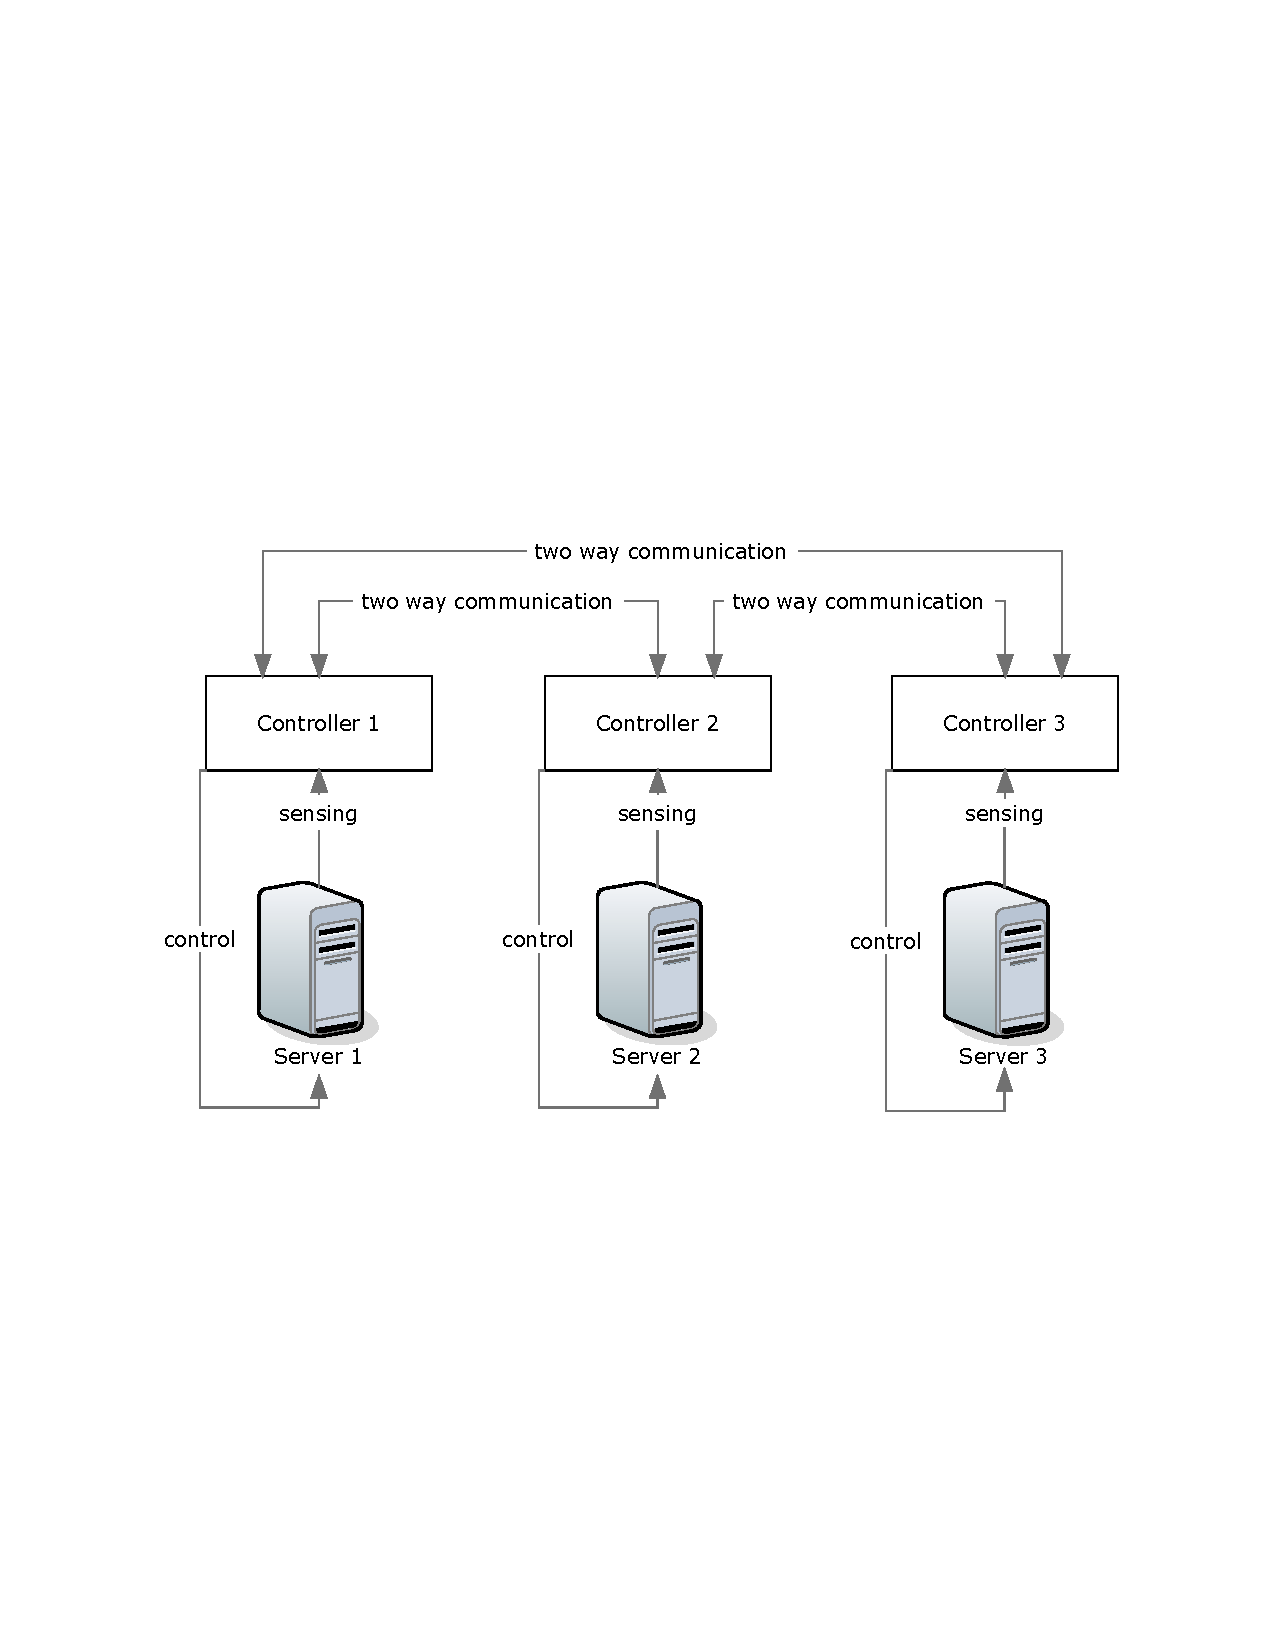
\includegraphics[width=0.75\linewidth]{ThesisRelatedArchiDecentralized}
	\caption{Decentralized Autonomic System Architecture}
	\label{fig:decentrarchi}
\end{figure}

Approaches to create such system range from biologically inspired architectures to self-organizing systems. Such an approach to build autonomic systems is that of a self-managing peer-to-peer architecture, as described in \cite{related:architecture:selfmanagep2p}. In this approach each element of the managed resource has its own management logic, and the overall Quality of Service (QoS) is achieved through peer-to-peer negotiation between the elements. While the architecture does distribute the management function across various elements, the architecture is not fully peer-to-peer, the authors choosing a hybrid approach. The top level of the QoS is reached through peer-to-peer negotiations, the lower level state is reached through hierarchical control. The described approach is meant for ``the autonomic management of heterogeneous networks and services'' \cite{related:architecture:selfmanagep2p}, but it can also be extended to other autonomic systems.

Another approach for developing decentralized autonomic systems is that of using biologically inspired architectures. In recent years, biologically inspired algorithms, like the Ant algorithm \cite{antalgorithm} for best route discovery in a network, have been investigated and developed. In \cite{related:architecture:selflet}, the authors propose an approach which is closer to biological models than to IBM's vision for autonomic systems. Instead of looking at an autonomic systems as a component that controls another resource, the authors design an autonomic system as a system that is able to change its internal behavior and its external interactions with other components, but is unable to modify external components. In order to reach this design, the authors create a ``SelfLet'' which is a self sufficient component, able to interact with other SelfLets in order to reach the high-level goals of the system. Each SelfLet has one or more behaviors, goals and actions. A goal represents a high-level objective, which can be achieved by executing some behaviors. Behaviors are performed by executing a set of local or remote actions. Similarly to the peer-to-peer architecture, SelfLets also have a negotiator manager, which they use in order to negotiate with other SelfLets a way to reach the goals.

Ant algorithms have also been investigated in autonomic systems. In \cite{statmechcomplexnetwork} the authors present an ant algorithm to decide where to place services in a cluster. Ants are created and sent in the datacenter to find available servers to use. As the ants traverse the servers in the cluster, they select servers where to deploy the service by examining each servers local state. Similarly, in \cite{messor:loadbalaneants} the authors use ant algorithm to determine load conditions and move jobs between servers in order to achieve load balancing in a data center.

In \cite{decentralized1} the authors use an approach similar to a peer-to-peer architecture. Each autonomic manager which comes online, for example for a new server starting, joins an autonomic management neighbourhood and exchanges messages periodically with members of the neighbourhood in order to determine the state of the system. Based on the information exchanged between autonomic managers, the autonomic managers can then make decisions on how to take actions to optimize the system. The authors apply the architecture to the grid problem of determining where to run various jobs in a grid while maintaining good performance for the various jobs running concurrently. In order to determine where to run the jobs, the system uses a neighbourhood of autonomic managers which decide the machines where jobs should be run, and, once started, monitor the jobs under their control to know the performance of the system. The managers also exchange information regarding the machines where jobs are being run and the performance of the respective jobs.

The decentralized approach has benefits in terms of scalability with respect to large systems, can be used for heterogeneous clouds and also works very well in systems where components can join and leave the system. As such, for the geographically distributed cloud presented in this thesis, the best approach is a self-organizing systems where each server manages itself and interacts with other servers in order to obtain a global optimal state for the entire cloud.

\subsection{Autonomic System Approaches}

In terms of approaches to creating the intelligent structure of an autonomic system, a variety of approaches also exists. Research into how to develop autonomic systems range from machine learning to control theory and include also policy based decision making, markovian models and economic models.

\subsubsection{Machine Learning}

Due to the fact that autonomic systems attempt to introduce intelligence into the management of the IT infrastructure, machine learning seems to be a very good approach to develop such systems. As such, machine learning methods have been widely used in research in order to create autonomic systems. 

In \cite{related:mldb} the authors use machine learning approaches in order to predict the performance of database queries using only information available before the queries execute. In order to achieve this goal, the authors examine five machine learning approaches: simple regression, clustering methods, principal component analysis, canonical correlation analysis and kernel canonical correlation analysis. The goal of the prediction was to try and compute, before a query is executed, and using only data about how the query is structured, and the query plan created by the database optimizer, multiple performance metrics such as CPU usage, memory usage, disk usage in order to be able to better predict resource contention in the database. Furthermore, the prediction had to perform well for both short running and long running queries, as well as for a database with a different schema than the trained database. The authors conclusions are that regression does a poor job of predicting the execution of SQL queries, in part because the regression algorithm ignored some of the query features when building the model. In terms of clustering, the authors conclude that for predicting both how long the query will take to execute and the performance characteristics of the query, they would need to run the clustering algorithm separately for each of the two datasets (execution time and performance characteristics). This approach would not find correlations between the two datasets. Principal Component Analsysis (PCA) has the same issue as clustering, as PCA can be applied only to a single multivariate dataset. Canonical Correlation Analysis (CCA) meets the authors goal of being able to find relations between pairs of multivariate datasets, however due to the fact that CCA uses an Euclidean dot product between the feature vectors of the two datasets to determine similarity the authors conclude that CCA is overly restrictive for the prediction of SQL query performance. Because of these restrictions, the authors use Kernel Canonical Correlation Analysis (KCCA) which is a generalization of CCA that uses kernel functions instead of Euclidean dot product for similarity measurement. The authors proceed to use KCCA in order to run experiments on a dataset constructed from a range of query types and obtain good results at predicting the performance metrics of the queries. 

A number of issues need to be noted about the work in this paper however. First of all, KCCA takes minutes to hours to train and, as such, the approach can not be used to re-train on the fly while the system is running. Second of all, the way the training dataset is constructed has major implications on the performance of the system as the machine learning algorithm will not be able to deal with anomalous queries which contain situations that did not exist in the training dataset. Finally, as the authors prove, it is very important to analyze the system which is to be managed as different machine learning approaches can be good for one management problem, but not for another.

In \cite{related:mlac} the authors develop a system which adds and removes servers from a cluster based on the cluster's workload by using a nonlinear regression model. The authors use a three step approach to predict the new number of servers to have in the cluster. The first step is to use a linear model to predict the next five minutes of workload based on the previous 15 minutes. It should be noted that no motivation is given for the use of 5 and 15 minutes respectively and that is unclear also how appropriate a linear regression is for workload prediction. While an ahead prediction of 5 minutes based on the last 15 minutes could be appropriate for the authors case, the same approach will most likely not work for all deployed clusters. The author's second step is to predict the required number of servers using the predicted workload as an input and a performance model, which is developed as a nonlinear regression model, to predict the number of required servers. Instead of trying to model all the parameters of the system, the authors prefer to detect whenever the model is no longer in sync with the system and create a new performance model from production data. In order to be able to use a new model, the controller of the system acts in two separate modes. In the first mode the controller acts very conservatively as it explores the production system in order to build the model. In this mode, the controller ensures that a very large number of servers are deployed in order to provide good performance and it slowly removes servers, trying to find the optimum. As the accuracy improves, the controller passes into the second mode called optimal mode in which the built model is used to add/remove servers based on workload predictions. It is easy to see that this approach causes suboptimal behaviour whenever the model has to be changed, as a large amount of extra resources which are not needed will be used. Finally, in step three the system determines how many new servers to add or remove. This is done based on the performance model's desired target but using a hysteresis approach with gains $\alpha$ and $\beta$ for adding or removing servers in order to avoid oscillations. $\alpha$ and $\beta$ are selected using apriori simulation runs (the simulations actually set $\alpha$ to 0.9 and find the corresponding $\beta$ value). The apriori selection of gains can also cause an issue since the model is chosen dynamically and previously selected gains can behave badly with a newer model. The system is simulated during an experiment on a pre-recorded workload of three days. The system manages to maintain the desired SLA (less than 5\% of requests have response times larger than 1s) and during the period the controller takes 55 add/remove actions. Looking at the authors performance graphs however, the system appears to be overcompensating while adding servers. Once a maximum number of servers is reached, even though the workload remains constant the system can remove servers safely and not cross the SLA parameters. This is caused most likely by the linear regression used for workload prediction.

Other machine learning approaches are those that use Bayesian models and neural networks. In \cite{related:model:ml} the authors compare the modelling of response time for a service-oriented architecture via Bayesian networks and neural networks. In order to build a Bayesian model the authors assume that each of the services is independent from all the others, and that the response time for the composition of the services is obtained due to a causal relation between it and the time elapsed on each service. As such, the authors use a Bayesian Network in order to model the systems response time.  Bayesian modelling is based on Bayes' theorem which states that ``the probability of a hypothesis H conditional on a given body of data E is the ratio of the unconditional probability of the conjunction of the hypothesis with the data to the unconditional probability of the data alone'' \cite{standford:bayes}. In terms of the response time modelling, this means that probability of a certain response time, given a distribution of elapsed times for each of the services is dependent on the prior known response time for the distribution and the conditional probability of that distribution. On the other hand, the neural network model is built as a feed-forward neural network, with six input nodes, six neurons in the hidden layer, and one output layer with one neuron. Figure \ref{fig:neuralnet} shows the structure of the neural network. In the neural network model, the various weights of how the inputs affect the hidden layer, and how the hidden layer affects the outputs must be found. Even though they are built differently, the two models have a number of common operations. Both models use newly measured data, both input and output in order to learn the system's behavior and improve the model. Thus the model must be able to receive new data and update itself. Furthermore, the models must be capable of being used in order to predict the future state of the output variables based on the the current state of the observed variables.

\begin{figure}
	\centering
		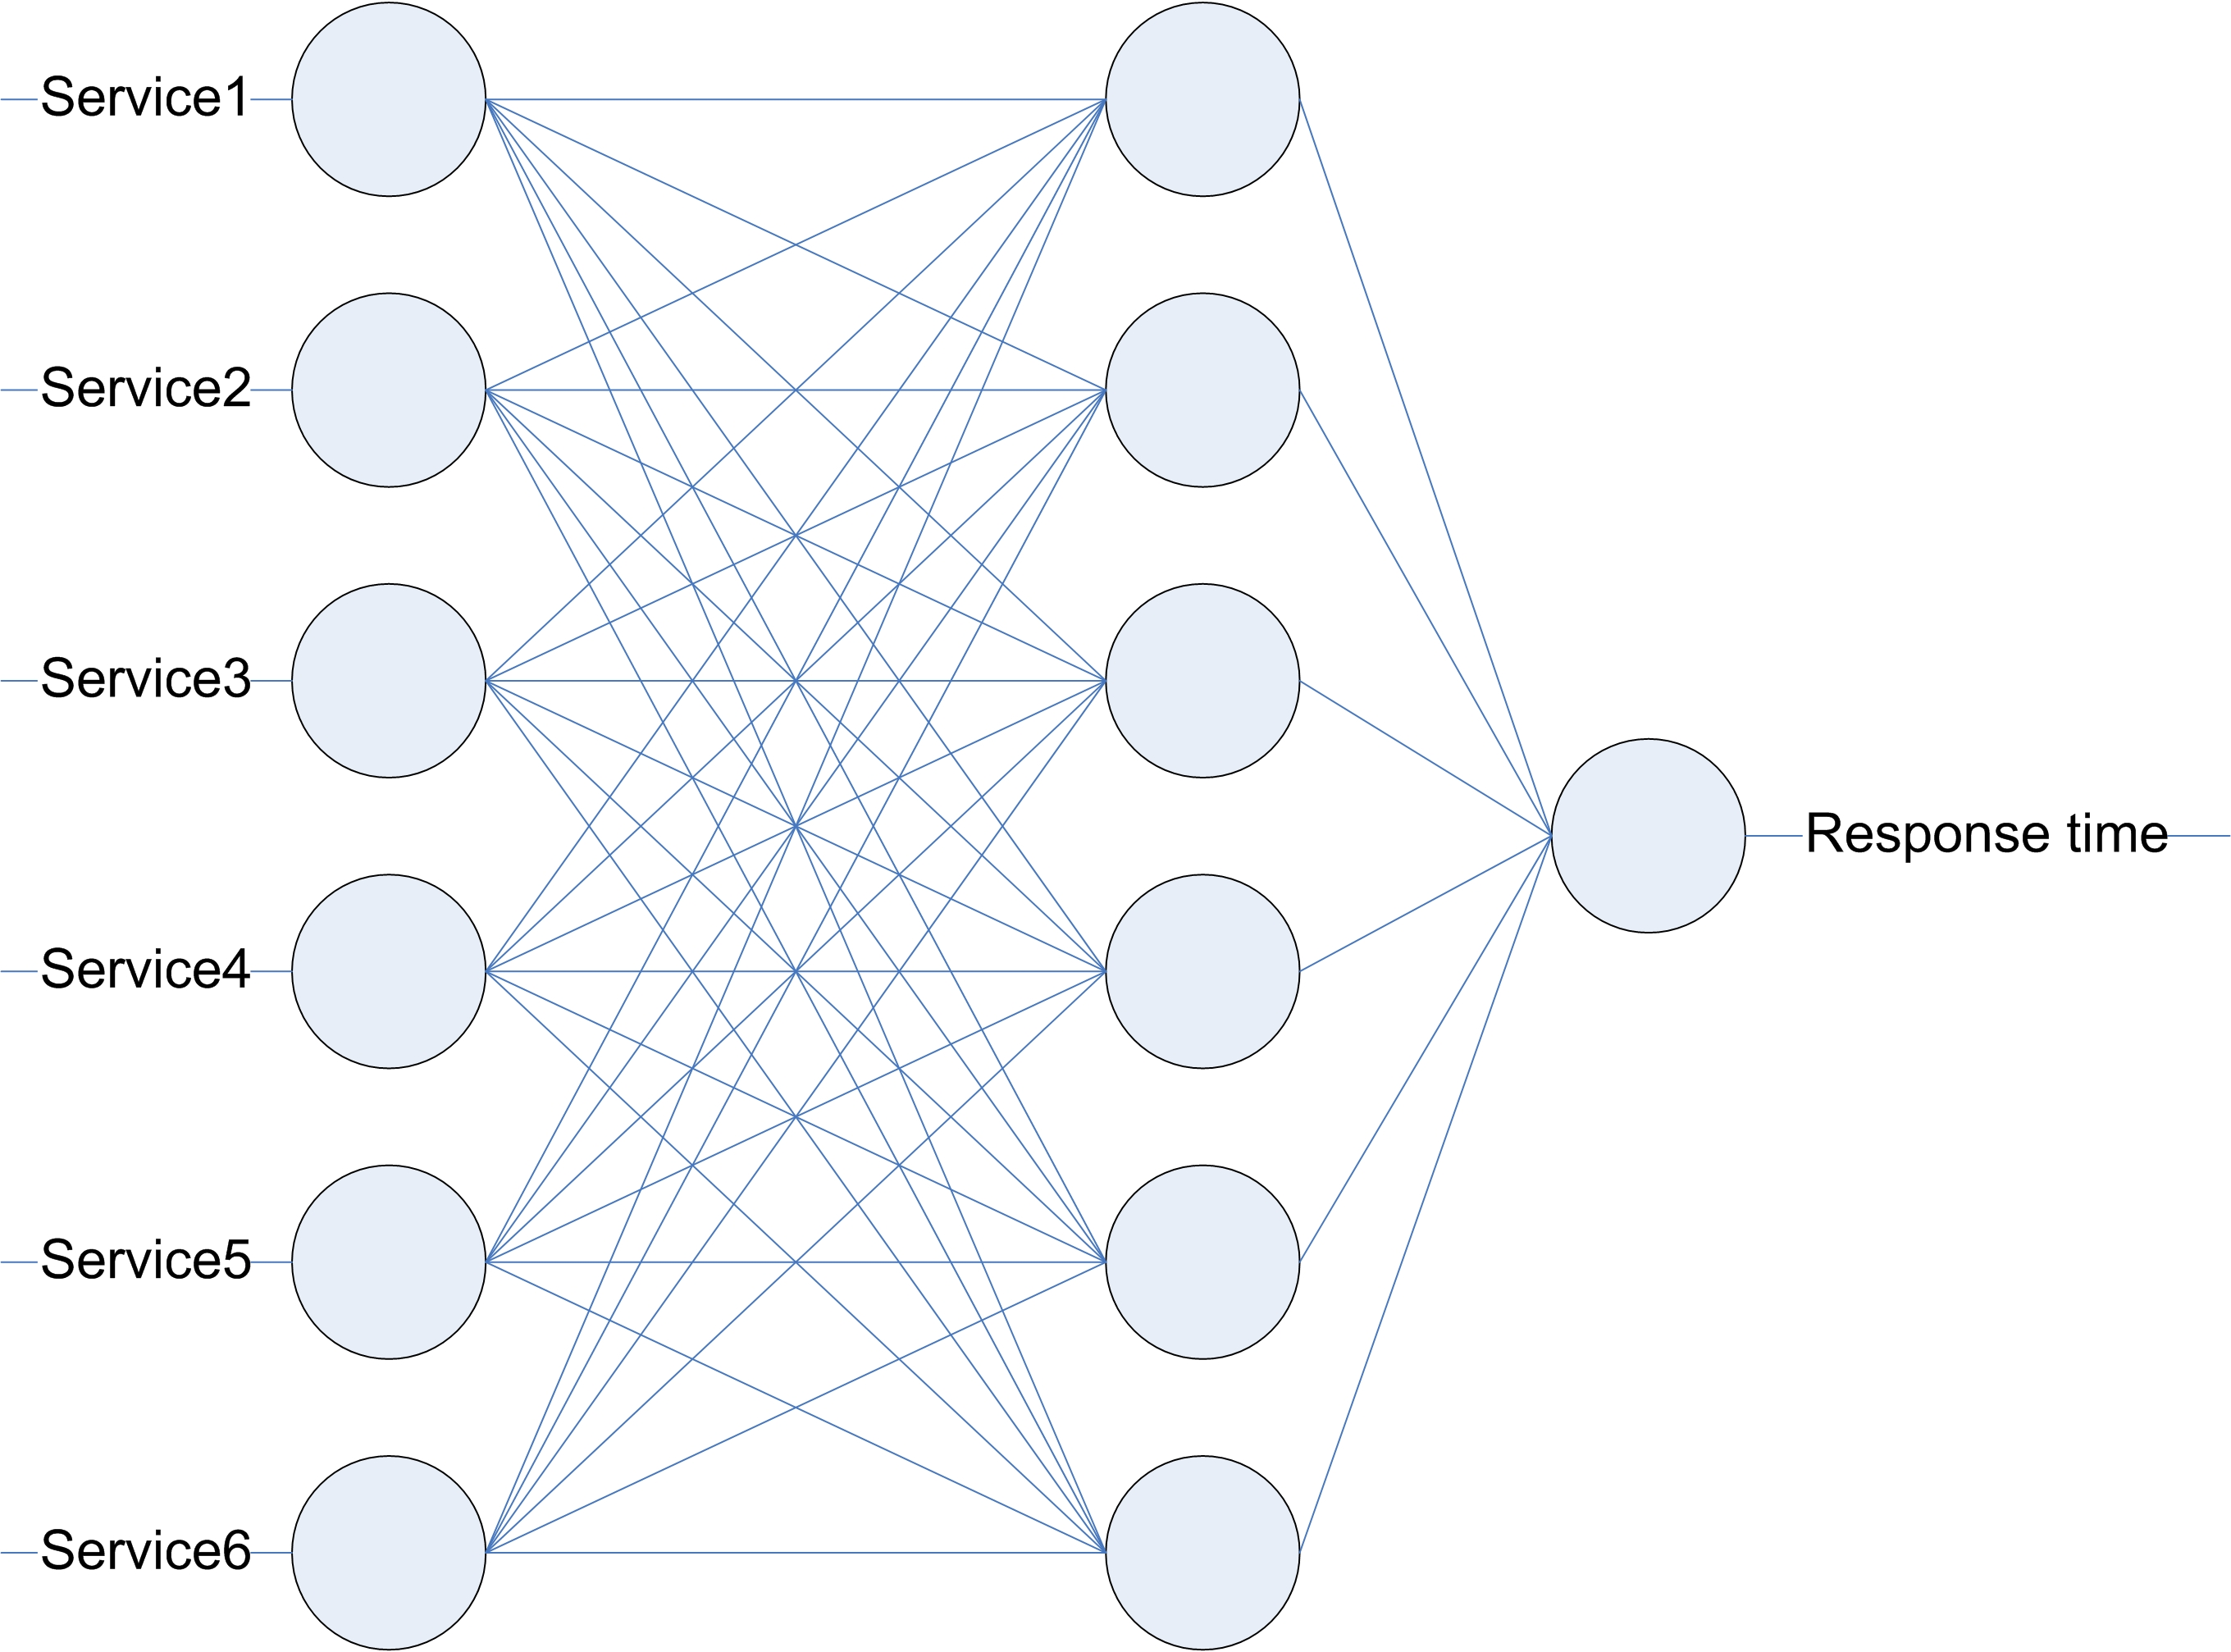
\includegraphics[width=0.65\linewidth]{neuralnetadapt}
	\caption{Neural Network Model}
	\label{fig:neuralnet}
\end{figure}

Similarly in \cite{related:bayesiandb} the authors use a Bayesian network in order to predict the response time of a database query or workload using a model which is built online and can be modified at run time. In order to achieve these goals, the authors use a Gaussian based response time model to encode the Bayesian probabilities. The Gaussian model is first trained offline and is capable of adapting itself once running online. Using a number of Gaussian models (linear and non-linear) the authors perform experiments on a database test bed and show the performance and robustness of the various models. One thing to note from the results is that all models have problems predicting queries that have not been seen before. Similarly, the models have problems making predictions when the online system is configured differently from the training system. 

\subsubsection{Layered Queueing Models}

A different approach taken to develop autonomic systems is to use Layered Queueing Models (LQM) to represent the behaviour of the system, and then to solve the LQM to predict the future state of the system. Autonomic Queueing Models base themselves on Queuing Network Model (QNM) theory, which sees an IT system as a network of queues such as CPU queues, I/O queues, network queues, etc. Requests to the system are split into a number of classes, where each class of requests exhibits the same behaviour with respect to the queues. The response time and throughput of the system can then be calculated based on the time it takes for the requests to go through the queues. A very important note about QNMs is that the structure of the queues can not be changed at run time and represents a static view of how the system must behave. As such any online adaptation in a QNM can only change the various parameters for the queues, but not the underlying structure of the queues and connections between queues. Figure \ref{fig:queueingmodel} shows a Layered Queueing Network with 3 nodes (each node has its own queue) in two layers. Arrivals into the system come into nodes 1 and 2, and from there requests move to node 3 from which the output is dispatched. Such a model can be used for two application servers with one database for example.

\begin{figure}
	\centering
		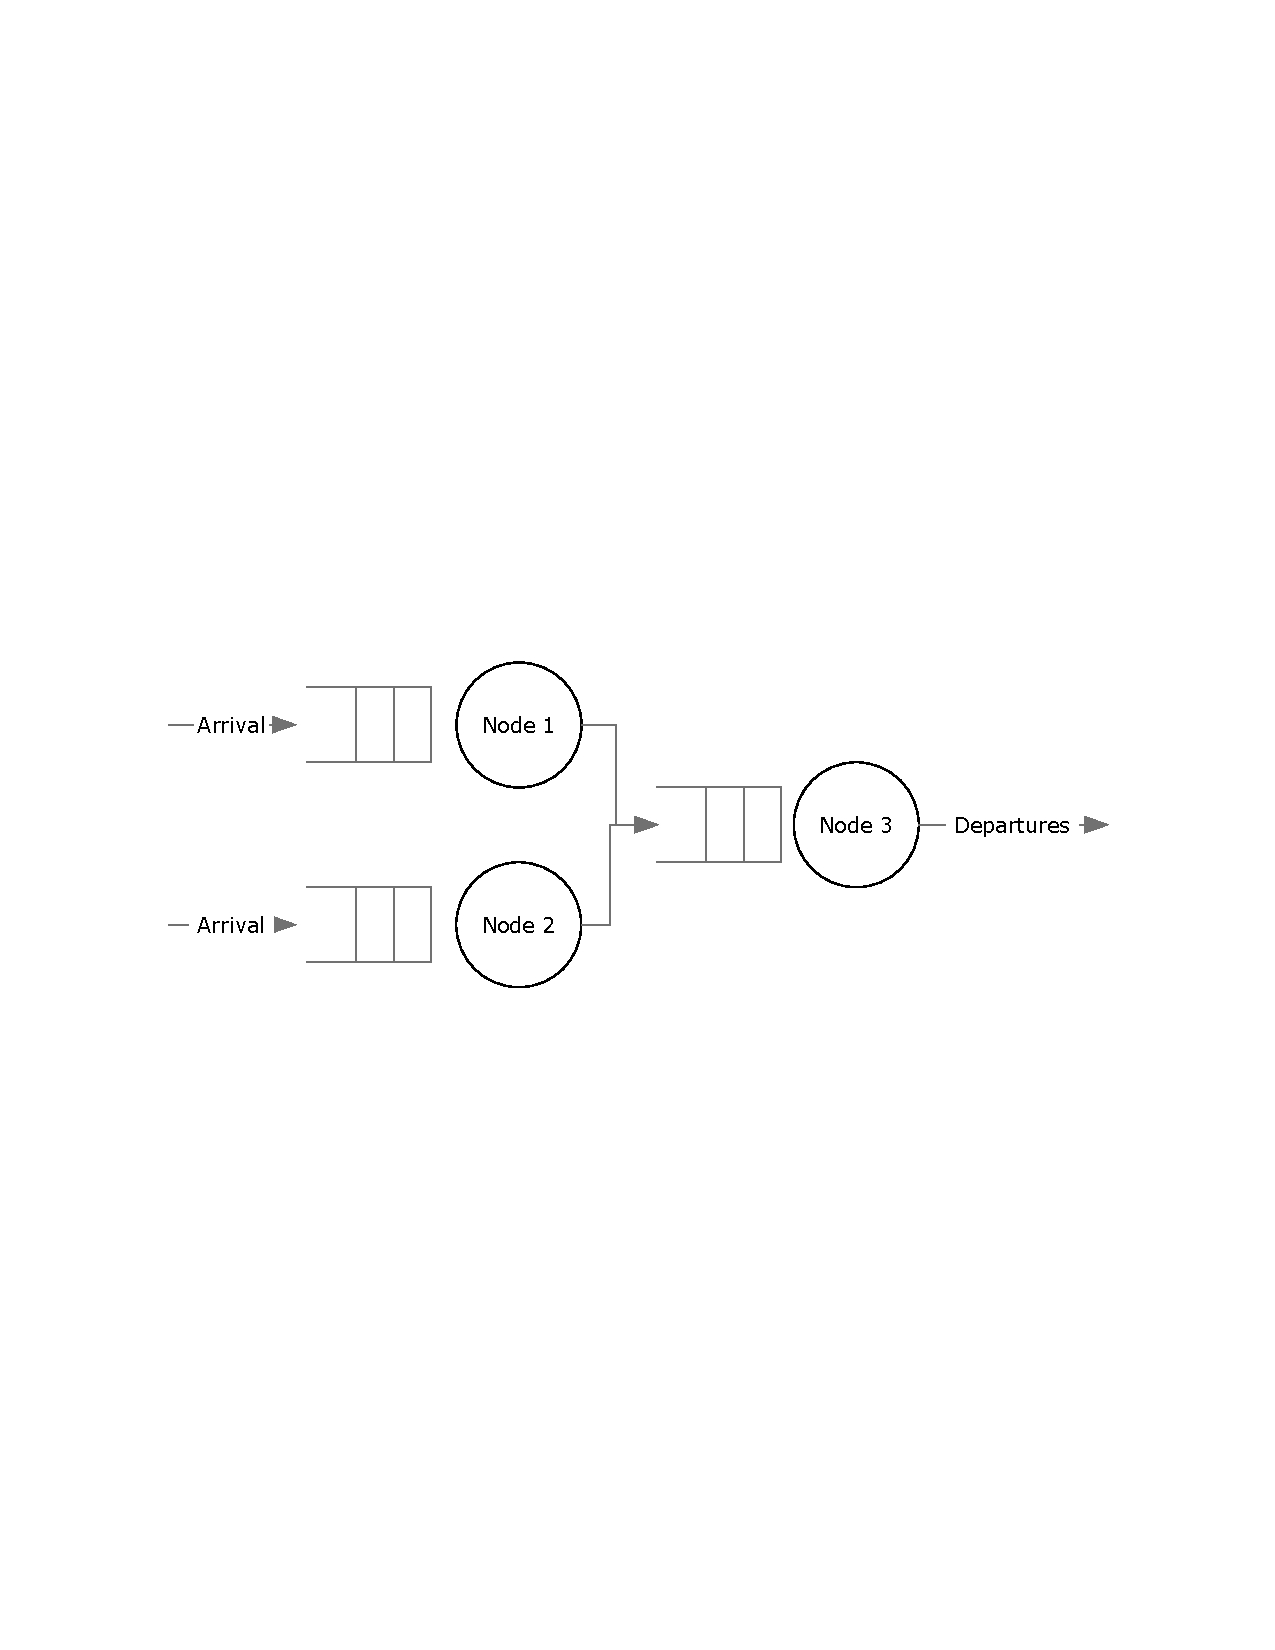
\includegraphics[width=1.0\linewidth]{ThesisRelatedQueueingModel}
	\caption{Layered Queueing Network Model}
	\label{fig:queueingmodel}
\end{figure}

Such an approach is taken in \cite{related:model:lqm} and \cite{related:model:lqm2} where the authors develop queueing models for multi-tiered transactional applications (i.e. a web server facing the client and sending requests for processing to an application server which uses a database to store and retrieve persistent data). In \cite{related:model:lqm} The LQM developed has a number of roles. First of all, the model is used to predict the future response time for each of the request classes by first predicting the future number of clients arriving in the system. If any of the predicted responses is outside the desired SLA, use the model to compute the number of servers which would alleviate the bottleneck since any high response is caused by bottlenecks at one or more of the queues. The new number of servers is computed using a hill-climbing algorithm. Finally, provision the new servers that alleviates the bottleneck problem. One thing to note, is that ``the forecasting step is in the order of minutes'', however there is no mention of what a good time period for forecasting would be or how various forecasting periods impact the forecasting accuracy. The problem in \cite{related:model:lqm2} is similar in that an LQM is build for a multi-tiered system. However, the authors develop a heuristic to try and maximize the profit obtained by the difference between revenues from SLAs and the cost of keeping servers on. This is done in part by load balancing when possible multiple similar requests to the same machines and by deciding which servers to allocate to which application tier. The authors approach is used to show results that suggest better performance than when using a proportional assignment schema. One issues that exists with this approach is that the algorithm takes a long time to find the maximum, and as such can only be run periodically and can not be used to continuously improve the system. At the same time, the authors choose a value of 60\% utilization as good utilization for the servers, but autonomic systems should attempt to obtain higher utilization in favor of using less machines, since it is preferable from an economical point of view to use one machine at 100\% than to use two machines running at 50\% each.

While the high-level modeling approach for the QNM  is very similar to the Bayesian models described previously, the differences appear in how the model is built and used. The Bayesian models output is based on the previously known probability of an observed distribution (past information on behaviour leads to the prediction of future behaviour), while the QNM's output is based only on the current size of the queues (present state of queues predicts future behaviour). The similarity between the models appears again regarding the functions that they perform. Both models are used in order to predict the future state of the system's output variables based on the current model state and a new input value, and both models can update their parametric model based on observed input and output values.

\subsubsection{Markov Chains}

A third approach, which appeared more recently in literature is that of using Markov chains, either discrete or continuous, in order to model the behaviour of the managed IT system. Figure \ref{fig:markovmodel} shows an example of a Markov Decision Process with 3 states and 2 actions. Each of the states can lead to any of the two actions, and from each action a certain probability leads to a different state. Some of the transitions have either positive or negative rewards, seen as the italic values next to some transitions.

\begin{figure}
	\centering
		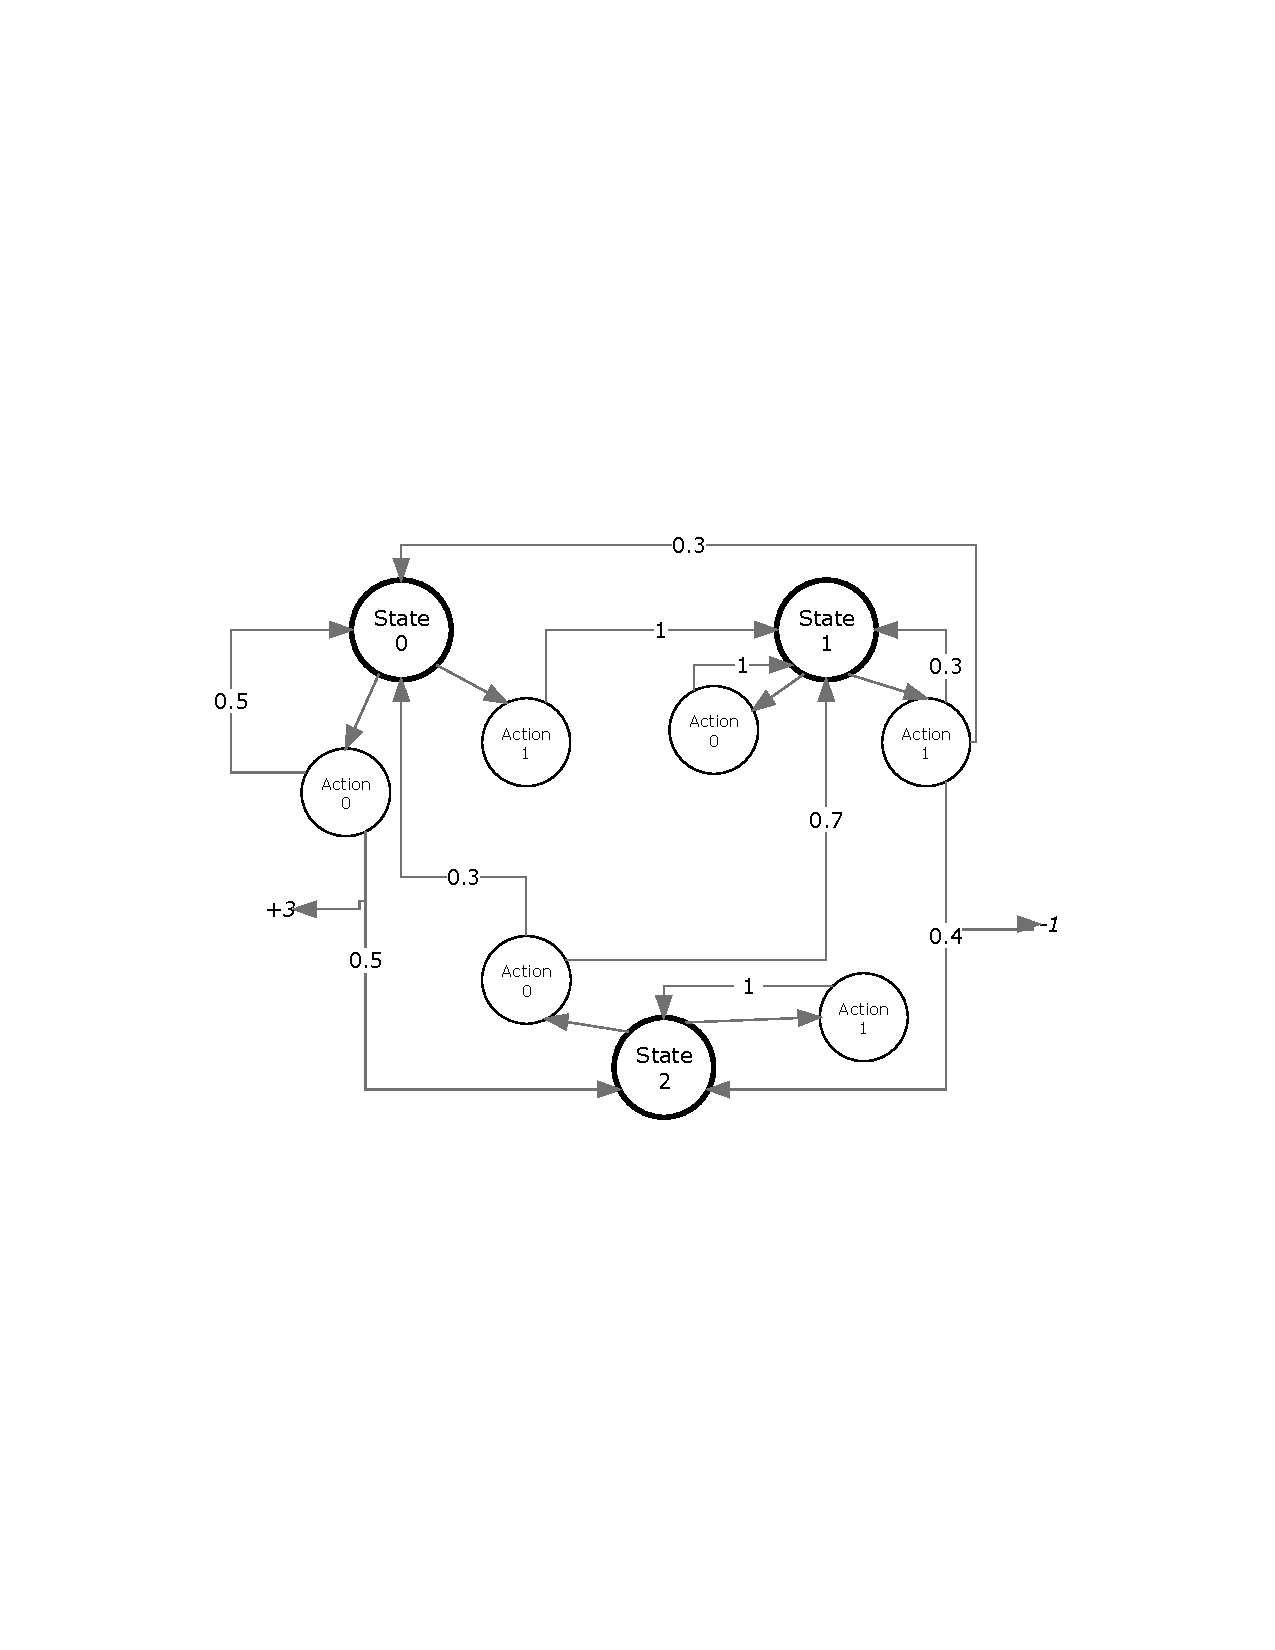
\includegraphics[width=1.0\linewidth]{ThesisRelatedMarkovModel}
	\caption{Markov Decision Process Model}
	\label{fig:markovmodel}
\end{figure}

In \cite{related:markov1} the authors introduce a framework for autonomic systems which uses Markov chains in order to model the system and by quantitative analysis of the Markov chain make decisions on how to adjust at run time the parameters of the IT system. In order to develop the system, the authors employ a probabilistic model checker/quantitative analyzer which uses a cost/rewards model to improve the parameters of the system. The autonomic system is applied to two autonomic problems. 

The first problem is that of dynamically managing the power of a hard drive by switching the state of the drive to sleep when it is idle. In experiments with the autonomic system, the management obtained using Markov chains performs better in terms of utility when compared to a simple timestamp method and N method. Also to note, the execution time of the autonomic system is sub-second but the CPU overhead is in the 1.5\% to 2.5\% range which is high for a problem like disk management. The second application of the autonomic system is for the adaptive management of a group of servers in which servers can be assigned to one of multiple clusters with clusters having different levels of SLA. The desired goal is to assign servers in such a way as to always reach the target availability of the most important cluster and trickle down in terms of cluster importance. For this purpose, a Markov chain is created for the cluster as well as a utility function which is to be maximized. A simulation is run with the described system and while the autonomic management ensures that each of the clusters has sufficient servers, the system does not deprovision unused servers. As such, the clusters have more servers than required. At the same time, based on the given results the system over-provisions the highest priority cluster by a large margin. In terms of execution, the authors mention that the system takes 30 seconds to compute the new state, which is an acceptable time to take, since provisioning servers takes an order of magnitude larger time to execute. A further issue is that it is unclear from the paper, if the system is reactive (changes the system once the SLA is breached) or proactive (predicts an SLA breach and changes the system before the SLA breach happens).

Similarly, in \cite{related:markov2} the authors use a Markovian decision process policy with reinforcement learning in order to perform resource allocation in a cloud environment. Markovian decision processes are an extension of Markov chains which allow for the existence of multiple actions for a state, thus including choice while going from one state to another, and of rewards, thus including a way to motivate the selection of a certain path. The goal of the system, is to manage a cloud datacenter, such that VMs are allocated in such a way as to maintain a required SLA for each of the applications running in the cloud while at the same time optimizing the number of VMs for each application. This problem is represented by the authors in the form of a Markovian decision process which takes into consideration the workload, the number of VMs allocated and the response time. Based on these values and the state of the decision process the system decides how many VMs to add or remove. One issue with a simple decision process is that the probability distribution functions are computed offline, and the system simply uses the predetermined functions to compute an optimal policy. The authors alleviate this problem by using a reinforcement learning approach to update the probability function by using rewards for good decisions. The authors apply the system on a simulation of a cloud with one application. The Markovian decision process system is capable to reach a policy which ensures that the SLA is maintained quite quickly. However, it is unclear if this allocation is optimal, since in the graphs the response time is 20 - 40\% lower than the required SLA, which could simply be due to over-provisioning of VMs. One interesting note of the authors is that long running systems will exhibit major changes in behaviour when the model has to be changed entirely since a reinforced learning system will not be able to react promptly due to the ``old'' knowledge in the system. At the same time, the authors note that the information used as input for the system is insufficient for appropriate decision making in the real world, as more data from the environment will be needed.

\subsubsection{Economic Models}

A similar approach to a punishment/reward system in order to make decisions is that of using economic models in policy making. Economic models consist of two actors: suppliers and consumers which use a trading mechanism to exchange resources. The trading mechanism is usually based on some form of ``currency'' which consumers use in order to obtain resources from suppliers. In \cite{related:econmodel} the authors apply an economic model in order to translate between business policy and low-level requirements for the automation of a database system. The control goal of the system is to tune the buffer pool of the database as well as the CPU usage when faced with multiple workloads. The workloads act as consumers and each workload has its own buffer pool and its own set of database agents, but the system does not have enough resources for all the workloads to execute quickly. Each workload has an estimated wealth based on the relative importance of the workload and the estimated work required for the workload, which is calculated based on the database's query optimizer prediction of I/O operations for the query. Using this wealth consumers (workloads) bid on resources dependent on the marginal utility provided by the given resources until either no more resources are available, the consumer uses all its wealth or the consumer has sufficient resources. A resource broker is used to enable the bidding process. The resource broker divides all the resources into blocks of resources which are up for bidding. For each of the resource blocks, the resource broker receives sealed bids from the consumers and chooses the highest bid. The bidding process repeats until no more resources are available, no more resources are desired by consumers or consumers do not have any wealth remaining. The above system is validated by running tests on an experimental environment. The economic model is first used to determine the resource allocation offline and the database is configured based on the results of the economic model. It should be noted that the system is not used to update the database's configuration online based on changes in workloads. The authors observe that the developed system is capable of obtaining effective allocations which result in similar number of reads to a system configured manually, which respect the desired importance of workloads and which result in the expected relative performance with respect to the relative importance values. One problem which the authors observe with the system is the fact that a real system would not know ahead of time the possible workloads (if such knowledge was available ahead of time manual configuration would be sufficient) and as such the utility functions would be hard to determine at run time. To create a really autonomic system a feedback loop would be required to obtain statistics from the running workloads and update the utility functions.

Another solution for autonomic systems is based on cost functions and optimization of such functions. In \cite{related:model:lqm2} which also uses a Layered Queueing Model and was described previously such a method is described. The authors assume that in a data center there are various costs: energy, hardware, and software utilization, as well as revenues obtained by providing the service and penalties due to breaches of SLA. The plan function is then based on the observation that ``revenues increase almost linearly with the system load and start decreasing after a maximum that is obtained when the service center utilization is about 0.5 to 0.6''. Because of this, the plan function attempts to optimize the cost function but since the optimization problem is NP-hard, the solution proposed is a heuristic search which results in a local optimum, but not necessary the global optimum. One important aspect of this paper is that it shows how multiple methods can be combined to create autonomic systems. In this case an economic based policy on top of a queueing model of the datacenter.

\subsubsection{Control Theoretic Models}

Due to the fact that autonomic system architectures are based on the MAPE-loop an approach to develop such systems which maps extremely well on the MAPE loop is that of using control theory methods and algorithms. One very important aspect of developing a system based on control theory (which also applies to some of the other methods) is that of creating a model for the system. Figure \ref{fig:blackbox} shows an example of a black box model for an application server. The arrival of clients acts as a perturbation on the system, which will change the internal state of the system which is hidden by the black box and in response to the state change the outputs of the system - CPU utilization and response time will be modified.

\begin{figure}
	\centering
		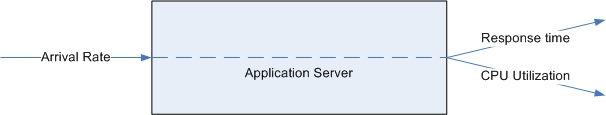
\includegraphics[width=1.0\linewidth]{BlackBox}
	\caption{Server Black Box Model}
	\label{fig:blackbox}
\end{figure}

The authors of \cite{related:control} explore how control theory can be applied to systems research in order to develop a management system for cloud computing environments. The authors note that such an environment, in which applications are consolidated across virtual machines and share dynamic resources based on the changing workload for the applications, pose a number of challenges to system administrators in the form of: ``complex SLAs, time-varying workload demands, distributed resource allocation and resource dependencies''. These challenges are addressed by using control theory in order to model, analyze and design a feedback loop for a resource management system. The autonomic system developed is applied to the problem of resource allocation in a shared virtualized infrastructure. The system does not provision new servers for the various applications, it just changes the resource allocations for the various virtual machines dynamically. The goals of the system are to guarantee application performance by reaching all the desired SLAs for the applications if possible (high demand periods could cause all resources to be used and low priority applications to miss their SLAs) and to provide high resource utilization and performance differentiation during contention periods (high priority applications maintain their SLAs over low priority applications). The authors identify six strengths of the control theoretic approach for autonomic systems, which are:

\begin{enumerate}
	\item Control theoretic systems offer a quantitative input-output model where a black-box model can be developed by performing offline experiments in order to determine the relation between the given control input, the perturbations in the system and the observed outputs which are the values to be controlled. Use of a proper input-output model in relation with a feedback controller offer the advantages of ensuring that the system converges towards equilibrium, that the system is stable and converges in appropriate time and that the controller can adapt to different regions of the input-output relation (for example if the input-output relation is bimodal).
	\item Control theory offers the ability to study system dynamics, which refer to the transient effects of past states on the current system state. Such input-output models can also be built by using system identification experiments to determine the degree of correlation between current output and past output values.
	\item Furthermore, using control theory system designers can develop multiple-input and multiple-output (MIMO) control models in order to capture the relations between the various inputs and outputs of the system. The relations in such systems are hard to quantify even when they are known.
	\item Control theory provides a number of well researched and well investigated algorithms for control based on models discovered via system identification for both single-input, single-output (SISO) and MIMO systems.
	\item Control theory also offers methods to determine the stability of the closed-loop model and control system. At the same time, control theory deals with the tradeoff between stability and responsiveness of the control system which is the tradeoff between how fast the system reaches a change decision and how stable the control system's decision is. A system which reaches decisions too fast will oscillate and be unstable as any small change in perturbations will result in a control decision. On the other hand a very stable system will make changes very slowly and miss important changes in perturbations.
	\item By using adaptive control theory, system administrators can develop controllers for systems with varying behaviour over time. This can be done by estimating the parameters of the model online and attempting to keep the parameters in line with the actual state of the system.
\end{enumerate}

For each of the six strengths the authors offer examples of how they applied control theory to various autonomic problems. The authors however, also note some limitations of control theory which must be taken into account while developing autonomic systems. First of all, computer systems exhibit non-linear behaviour which makes modelling more difficult. Second of all, the development of black-box control models requires very controlled experiments to be run. Such experiments can not be usually run based on data from production systems since such data rarely contains the required perturbations or constraints to determine the relations between input and output. Third of all, classical control theory deals with continuous inputs. While discrete values can be quantized, this can lead to instability or inefficiency. Finally, classical control theory usually deals with tracking problems - the control system maintains a variable at a certain value. For autonomic systems, the goal is generally to maximize or minimize some values (maximize resource usage while minimizing response time for example). Any person who creates autonomic systems by using control theory must take these limitations in consideration and deal with them.

Similarly, in \cite{related:control2} the authors compare various approaches to creating decision makers for autonomic systems. They look at heuristic approaches, standard and advanced control-based approaches as well as model-based and model-free machine learning approaches. In order to compare the five methods the researchers look at a standard autonomic computing problem, namely the problem of resource allocation to some running application in an operating system. The application which is assigned resources has a way to signal ``heartbeats'' at important places in code as well as to describe desired performance goals. The authors conclusion is that an adaptive control approach like a Kalman Filter produces good results for a range of applications, and this matches the observations of \cite{related:control}. The authors note that for a given system with a narrow range of behaviours testing multiple approaches is the best approach, for a system with a broad range of behaviours or even unknown behaviour ahead of time (a self-optimizing application server with unknown applications running on top) adaptive control is the best approach.

The issue of applying control theory methods for managing the CPU shares received by multiple resource containers running on the same machine is addressed in \cite{related:control3}. Resource containers are a way to provide performance isolation for applications running on the same hardware and they can be either an operating system feature or an entire technology like virtualization. Usually the resource container resource allocation is done offline before deployment and does not change during the lifetime of the applications. The authors present an approach to change the resource allocations dynamically by using a feedback control loop based on control theory principles. The specific application under control in this case is an Apache Web server running inside HP-UX PRM as a resource allocation system. The model of the system is created by applying system identification on observable metrics for a black-box model. The reason to use a black-box model given by the authors is that the complexity of a web server makes it hard to obtain a control model from first principles. The model for the system is a SISO model which correlates the CPU usage of the resource container to the Mean Response Time (MRT) of the web server. The system identification is done using a single workload meant to stress the CPU of the container. Using the model obtained by system identification, the authors apply a simple Proportional-Integral (PI) controller and show that such a system is stable, has a rise time of 3 sample periods and settling time of 6 sample periods. The rise time refers to the time it takes for the controller to respond to a change in perturbations, while the settling time refers to how fast the controller reaches stability after a perturbation.

The problem with the PI controller is that it is ``trained'' through system identification on one workload and would not respond very well to a different workload. In order to deal with unknown workloads the controller must be developed using adaptive control. This observation matches that of \cite{related:control} and \cite{related:control2} which note that adaptive control is best for systems with unknown behaviour ahead of time or for those with changing behaviour. The adaptive control is applied to the system by adding a parameter estimator for the model discovered using system identification. The two parameters are estimated using the recursive least-square (RLS) method and are updated at each interval. The parameters are then fed into a pole placement module which chooses the desired parameters of the PI controller in order to have the poles of the transfer function at the desired location. The two control systems (adaptive and simple PI) are evaluated on a test-bed. The simple controller is capable of maintaining the response time within 15\% of the target value when being faced with a workload similar to the one used for system identification. The adaptive controller is capable of maintaining the response time within 20\% of the target value even with changes in the workload. However, the tradeoff is that the convergence towards the desired response time is slower using the adaptive controller and that this controller also oscillates more. The simple controller is not tested on the varied workload since its results would be bad.

\cite{related:control4} deals with a similar issue, that of developing a feedback control system for managing the service delay (response time) for web servers based on relative or absolute delay guarantees. Absolute delay guarantees require that each class of services is served within the desired time when the server is not overloaded. When the server is overloaded admission control is applied based on some form of priority order over the services. In relative delay a fixed ratio between the delays of the various classes is maintained. The problem with ensuring such guarantees is that the workload is unknown ahead of time, and as such developing a robust control system for service delay guarantees is complicated. Two types of controllers are used in the proposed system - one for relative and one for absolute service delay. The absolute delay controller uses a PI controller similar to the work in \cite{related:control3} and the control parameters are determined using system identification. The relative delay controller computes the relative delay between two adjacent classes. Thus the system contains n-1 controllers for n classes of services. Each of the controllers uses a PI controller with extra logic on top to calculate the ratio of the two service classes under control. Similar to all the other control theoretic papers, the authors note that such a system would face problems if the workload during deployment is vastly different from the workload on which system identification was done. In order to alleviate this issue one can use adaptive control. The system is applied to a testbed of Apache Web Servers for both absolute and relative delays with two and three classes. The experimental results show that the control method is capable to reach the desired guarantees when run in a closed-loop, while the open-loop solution violates the desired delays when the workload changes.

Similar work is performed in \cite{related:control5} where the issue of managing the database connection pool in a web server is approached from a control theoretic point of view. The goal of the work is similar to that of \cite{related:control4} in that the system's final goal is to improve the response time of a server under heavy load. Unlike \cite{related:control4} this is achieved by setting priority for the idle connections in the database connection pool, however similar to \cite{related:control4} this is done by using the dual approach of proportional delay differentiation and absolute delay differentiation. Like \cite{related:control4} the authors use system identification to determine the PI controller's parameters by applying the RLS method. The system is tested on a server running Tomcat and the system is capable to maintain the desired response time in the face of varying workloads.

Based on this work a number of observations about control theory for autonomic systems can be observed. First of all, all research in autonomic systems control theory has focused on developing black box models due to the difficulty of applying first principles to IT systems. Second of all, most researchers focus on using simple controllers like the PI controller for autonomic systems and use experiments and system identification in order to find the parameters of the controller. In order to deal with varying perturbations, researchers apply adaptive control on top of the simple PI controller.

\subsection{Self-organizing Systems}

Self-organizing systems deal with complexity in management systems by allowing the management of the system to appear from the interaction between the components of the system. Such systems have no global controller and components do not have access to information outside their own local information. Components can however exchange messages with each other to inform other components about the sending component's state. Through this, ``emergent'' behaviour appears in systems, behaviour which is not imposed from outside the system. Like autonomic systems, self-organizing systems are inspired by behaviour observed in nature like ``synchronous flashing that sometimes develops among aggregations of thousands of fireflies in southeast Asia'' or the stripped and mottled pattern which appears in zebras and fishes. Experiments and theoretical work suggests that such apparent complex patterns appear from a small number of very simple rules and research into them can be found in \cite{related:selforganization-honeybee}, \cite{related:selforganization-autoscaling}, \cite{related:selforganization-autoscaling2}, \cite{related:selforganization-plant}, \cite{related:selforganization-healing1}, \cite{related:selforganization-healing2}, \cite{related:selforganization-energymanagement}.

The problem of the stripped pattern was examined in computing by Alan Turing who first suggested in 1952 the general schema for this mechanism of self-organized pattern formation. The self-organizing system has a number of sites which act as activators. The activators produce two pheromones: a short range activator which enhances the activator production and a short range antagonist which ensures that the self-enhancement is localized. By performing simulations using a model of such a system both stripped and mottled patterns can be obtained. This shows that complex behaviour can emerge from very simple rules through the collaboration of components.

Self-organizing systems were also employed by Ashby to create his homeostat \cite{ashby:homeostat} which is capable of adapting itself to any perturbation in the system and reach back a stable state. The initial system built by Ashby was an adaptive ultra-stable system with the goal of showing Ashby's law of requisite variety, which states that a control system needs as many internal states as those of the system being controlled. The system automatically adapted its internal configuration to stabilize any disturbance introduced in the system. Figure \ref{fig:homeostat} shows the output of a homeostat. As any of the four pens is perturbed, the system self-organizes until all four pens are back to a stable state.

\begin{figure}
	\centering
		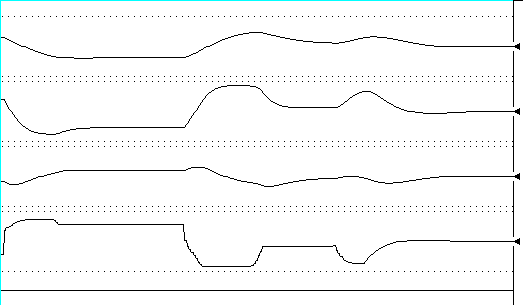
\includegraphics[width=1.0\linewidth]{homeostat}
	\caption{Homeostat}
	\label{fig:homeostat}
\end{figure}

In \cite{selforg:survey}, the authors look at a number of self-organizing algorithms and compare them in the context of the problem of load balancing requests in a cloud environment. Some of the algorithms examined include Particle Swarm Optimization, Artificial Bee Colony, Genetic Algorithms and Ant Colony Optimization. Furthermore, the authors examine in detail the Ant Lion Optimizer algorithm for load balancing due to it's better performance and better ability to search the entire solution space instead of falling into a local optima. The authors observe that the self-organizing algorithms perform better than traditional algorithms in terms of quality of service provided and minimize the response time, at a tradeoff of more network and processing overhead.

\subsubsection{Genetic Algorithms (GA)}

One of the oldest approaches for self-organizing systems is based on mutating solutions and maintaining only the fittest solutions to continue mutating in the future. The optimization usually starts with a random solution which is encoded in some form of digital representation - usually a binary string. There also exists some form of fitness function which decides how good a solution is. Solutions are chosen in pairs and they exchange part of the solution to form two children. Mutations can also be introduced by randomly changing part of a child. After the population of children is obtained, the children are measured using the fitness function and unfit children are removed from the population. The surviving children become the new parents and the loop is repeated either for a given number of iterations or until a certain fitness value is passed. The final solution is the one with the best fitness of the entire population. The pseudocode in \ref{algo:ga} shows the behaviour of GA algorithms.

\begin{algorithm}
\begin{algorithmic}
\State Random generation of initial parents
\While{end criteria not met}
	\State Select parent pairs and cross over chromosomes
	\State Randomly mutate children
	\State Compute children fitness
	\If{child is fit}
		\State keep child in population
	\Else
		\State remove child
	\EndIf
	\State replace parents with children population
\EndWhile
\State return best fit child
\end{algorithmic}
\caption{Genetic Algorithm Pseudocode}\label{algo:ga}
\end{algorithm}

In the case of the problem presented in this thesis - that of optimizing the size of a cloud of servers dynamically at runtime - a GA could encode the servers to be used as a binary array of 0 or 1, and then find the best solution in terms of future performance of the system by predicting which servers should be up (a 1 in the binary array) or stopped (a 0 in the binary array). The GA can not be used in order to determine when the system is about to breach its SLAs, and can only be used in order to obtain a new optimal state. At the same time, GAs are known to be slow in order to obtain a good solution as the number of iterations taken to converge can be very large if a good solution is desired. As such, GAs are not a very good fit for a real time self optimization of cloud resources.

\subsubsection{Particle Swarm Optimization (PSO)}

Particle swarm optimization uses as inspiration the behaviour of flocks of birds or swarms of fish looking for food. Each possible solution represents a particle in the search space with a position, and the particles move based on their own speed and the best known position. At the same time, there exists an optimization function $f$ which takes as value the position of a particle and returns a value representing how good that solution is. As such, each particle is initialized with a random position and speed. Each of the position computes it's $f$ function and save it as the position's best solution. The best of the $f$ values is stored as the swarms best solution. At each step of the iteration, each of the particles computes a new speed and a new position based on the previous position and speed, such that each particle's movement is guided by it's own best solution and the swarms best solution. Once an exit criteria is reached - either number of iterations or the desired function is sufficiently improved, the algorithm exits and the best swarm position is used as the solution of the optimization problem. The pseudocode in \ref{algo:pso} shows the behaviour of PSO algorithms. $f(swarm)$ is defined as the best solution for the swarm.

\begin{algorithm}
\begin{algorithmic}
\State Random uniform generation of initial positions and velocities in search space
\ForAll{Particles} 
	\State Compute particle's position and save as best position
	\If{$f(particle) > f(swarm)$} 
		\State update $best(swarm)$ = particle
	\EndIf
\EndFor
\While{end criteria not met}
	\ForAll{Particles} 
		\State Compute particle's new speed
		\State Compute particle's new position
		\If{ $f(particle_{new}) > f(particle_{best})$ } 
			\State update $particle_{best}$ = $particle_{new}$ 
		\EndIf
		\If{ $f(particle_{new}) > f(swarm)$ } 
			\State update $best(swarm)$ = $particle_{new}$
		\EndIf
	\EndFor
\EndWhile
\State return $best(swarm)$
\end{algorithmic}
\caption{Particle Swarm Optimization}\label{algo:pso}
\end{algorithm}

For example, a PSO is used in \cite{selforg:pso} in order to obtain the initial placement of tasks in a cloud. The system described in the paper does not perform any real-time optimization and only takes care of the initial problem of placing N SaaS tasks on M cloud instances, where $M < N$. The system uses a position vector to describe which task is assigned to which server and then uses the PSO algorithm to find the best placement.

Similarly to the GA algorithm, the PSO algorithm can not be used in order to detect when a system breaches it's SLA and can only be used once some other system detects a possible SLA breach. PSOs can also fall easily into local optima depending on how well the parameters of the problem are set at the beginning. If the parameters cause too small speed/position changes than the system can fall into local optima easily. If the parameters cause large changes then the optimization problem can fluctuate.

\subsubsection{Artificial Bee Colony (ABC)}

The artificial bee colony algorithm \cite{selforg:abc} is inspired by the process used by a honey bee swarm in order to forage for food. Unlike in other self-organizing systems, not all the composing parts are the same in the ABC algorithm. Three types of bees are used in the algorithm: employed bees, onlooker bees and scout bees. The problem to be optimized is defined in terms of food sources, with different solutions representing different food sources. For each source of food there is one employed bee which goes to that source, forages and returns home. Onlooker bees stay at the nest and establish new food sources based on the information received from employed bees returning to the hive. Onlooker bees choose new food sources by watching the employed bees come back to the hive in the dancing area, and perform a dance based on how good the food source is. Finally, scout bees establish new food sources via random searching around the hive.

Algorithmically, this behaviour is represented by an iterative loop over three phases: employed bee phase, onlooker bee phase, scout bee phase. Initially, the food sources are initialized by having the scout bees go and find random solutions in the solution space. In the employed bee phase, employed bees generate new solutions by going to an existing solution and searching the space around it for a new solution. Once a new solution is generated, the fitness of the new solution is computed and a greedy algorithm used to choose between the new solution and the original source. Employed bees then go to the hive and share the information with onlooker bees in the dancing area. In the onlooker bee phase, onlooker bees choose their food source based on the information received from the employed bees. Once an onlooker bee chooses a source, it also determines a neighbour and computes the fitness of the new solution and chooses between the new solution and the old. In the scout phase, employed bees which can not improve on their solution after a number of iterations give up and become scout bees. Scouts search for solutions randomly.

The pseudocode in \ref{algo:abc} shows the behaviour of ABC algorithms.

\begin{algorithm}
\begin{algorithmic}
\State Initialize solutions randomly using scout bees
\While{end criteria not met}
	\State Employed bee phase
	\State Onlooker bee phase
	\State Scout bee phase
	\State Store best solution up to now
\EndWhile
\State return $best(solution)$
\end{algorithmic}
\caption{Artificial Bee Colony}\label{algo:abc}
\end{algorithm}

Like the GA and PSO algorithms, this algorithm can not be used to detect problems in the system, and can only be used to obtain an optimal solution to the problem at hand. Compared to both GA and PSO, ABC offers similar or better performance but with less control variables needing to be used - thus creating a simpler algorithm to implement.

\subsubsection{Ant Based Algorithms}

Similar to the ABC algorithm, the ant colony optimization (ACO) algorithm is inspired by the behaviour of insect hives - in this case ants. The behaviour which inspired this algorithm is the way in which ants can build an efficient path between the nest and a food source using random search and reinforced learning. In real life, ants randomly search for food around the nest. When an ant finds a food source it returns to the nest with some food while laying a pheromone trail. Other ants which meet the pheromone trail are more likely to follow the trail then continue searching randomly. If the food source is large enough eventually a large number of ants follow the same path as each ant lays down a pheromone trail causing more ants to follow it. At the same time, the pheromones dissipate over time such that once a food source is depleted and ants no longer return with food from it, the trail will disappear. 

The ACO algorithm is very similar to the behaviour of ants in real life and is best used to find optimal paths through graphs. For example, the algorithm has been used to provide reinforced learning for routers in a network for better packet forwarding \cite{selforg:aco}. In simple terms, the ACO is composed of a number of ants which are traversing the network by moving from node to node across edges. As ants move through the network they deposit pheromones on the edges based on some function. When ants decide the next node to go to, they choose based on the pheromones on the nodes going out from the current node. The selection of the next node is done pseudo-randomly such that not all ants follow the same path, however more ants will prefer edges with higher pheromone levels. 

In the case of routing in a network, the nodes are the routers and the edges are the connections between the routers. Ants are packets being sent between the routers and either they wait in a normal queue or have higher priority than normal packets. If the ants simply wait in the queues to be processed then they can measure the processing latency at the routers. As ants traverse the network they can update the routing table with information regarding how loaded is the network and also the best routes between different nodes. The pheromones in this case act as a way for more ants to go through low loaded network links such that those links are used by normal traffic.

The pseudocode in \ref{algo:aco} shows the behaviour of ACO algorithm from the perspective of an ant.

\begin{algorithm}
\begin{algorithmic}
\While{end criteria not met}
	\State Find next node based on pheromones/random
	\State Go to next node
	\State Update pheromones for the edge just traversed
\EndWhile
\State return $best(solution)$ based on pheromones
\end{algorithmic}
\caption{Ant Colony Optimization}\label{algo:aco}
\end{algorithm}

Another self-organizing algorithm is based on the behaviour of ants when relocating to a new nest in the case when the old nest was destroyed. This behaviour is similar to that of honey bees when relocating \cite{selforg:antreloc}. When their nest is destroyed, ants start looking for a new nest by doing tandem runs. In such a case, there are two types of ants - scouts and non scouts. Scouts start to search for new nests randomly and upon finding a new possible nest they determine how viable the new nest is and return home. Upon coming back home ants recruit from the non-scout ants and do tandem runs together. At the same time scout ants can be recruited by other scouts who have a better nest as their new nest. This process is repeated until a quorum of ants has chosen a new site for the nest. Ants can give up on their possible new nest if the population of the new nest starts decreasing - suggesting that ants from this new nest have been successfully recruited by a better nest. The pseudocode in \ref{algo:antreloc} shows the behaviour of the ant relocation algorithm.

\begin{algorithm}
\begin{algorithmic}
\State Round 1: Ants find new nests
\While{more than one nest}
	\State Round 2: Viable ants return home and recruit from the other ants
	\State Round 2: Not viable ants wait one turn
	\State Round 3: Tandem runs to new nest. Upon arrival at new nest ants compare previous and new nest size. Nest with decreasing pop become not viable. 
	\State Round 3: Not viable ants return home
\EndWhile
\State return $single nest$
\end{algorithmic}
\caption{Ant Colony Relocation}\label{algo:antreloc}
\end{algorithm}

The main reason to use self-organizing systems for autonomic system development is that the two have a number of characteristics in common like the ability to deal with unexpected changes in the environment. Unlike the other self-organizing systems presented, the ACO algorithm can be used to detect when the system breaches or is about to breach it's SLAs. As ants move around the system, they can take measurements and approximate the state of the entire cloud based on their knowledge of the pheromone levels across the cloud. Once a certain threshold is reached ants can trigger a request for self-optimization which is computed by a separate algorithm. Because of these reasons, this thesis will use the ACO algorithm to develop the self-organizing, self-optimizing system.

\subsection{Cloud simulation systems and benchmarks}

In order to test any proposed system and prove the performance of the system, the system must be run either on a simulation or on a live test bed. For cloud systems it is especially difficult to use a live test bed as a large number of servers or resources must be used at a significant cost. As such, a number of simulation platforms have been developed by various research groups. Furthermore, in order to be able to show that one solution is better than another a comparison must be done between different solutions.

A number of cloud simulation frameworks were developed by various research groups in order to allow for validation of various cloud algorithms. Example of such systems are CloudSim \cite{related:cloudsim}, GreenCloud \cite{related:greencloud} and iCanCloud \cite{related:icancloud}. GreenCloud is ``a sophisticated packet-level simulator for energy-aware cloud computing data centers with a focus on cloud communications''. iCanCloud is ``a simulation platform aimed to model and simulate cloud computing systems'' whose goal ``is to predict the trade-offs between cost and performance of a given set of applications executed in a specific hardware, and then provide to users useful information about such costs. '' The goal of CloudSim ``is to provide a generalized, and extensible simulation framework that enables seamless modeling, simulation, and experimentation of emerging Cloud computing infrastructures and application services.''

Because of the fact that GreenCloud focuses on cloud communications and iCanCloud focuses on the initial deployment of cloud resources, the simulation system used in this thesis is CloudSim as the simulation framework used to validate the self-organizing algorithms introduced. CloudSim together with the CloudSimEx extension allows the user to create an initial cloud structure - hardware hosts as well as VMs running on those hosts, create a workload and then simulate the behaviour of the cloud. The CloudSimEx extension adds the capability of simulating web sessions and also adding an auto scaling policy. A simple auto scaling policy based on CPU usage is provided out of the box by the CloudSimEx extension.

In order to show that the proposed system behaves better than other proposed solutions for auto scaling of clouds the system's performance must be compared to other such scaling systems. In order to achieve this it is desired to use common benchmarks and workloads, such that all systems are compared under similar circumstances. Unfortunately no such benchmarks and workloads exist for cloud systems and for cloud auto-scaling - with every researcher defining their own test sets. As mentioned in \cite{related:cloudbench}: ``Authors use different ways of generating input workload, different types of applications (realistic or simulated), different SLA definitions, different execution platforms, etc. In fact, the lack of a common testing platform capable of generating a well-defined set of standardized metrics is the reason that prevented a comparative analysis of the reviewed techniques in quantitative terms.''. Because of the lack of existing benchmarks it is impossible to compare the proposed solution with the solutions provided by other research groups, and as such the thesis will compare the auto-scaling mechanisms proposed with simple auto-scaling policies offered by various providers like Amazon, Google, etc. similar to the comparison done in \cite{related:clousimex-scaling}.

\section{Related Work Conclusions}

The goal of this thesis is to develop a self-optimizing system which manages the elasticity of cloud resources. Investigation into related work have lead to a number of conclusions. 

\begin{itemize}
	\item The best approach to create an architecture for such a system is to use a decentralized self-organizing architecture which scales well with large numbers of servers in the cloud.
	\item The system must be able to manage not just the CPU usage but other measurements like response time and latency as seen by end-users which are very important in certain applications.
	\item A modified version of the ACO algorithm can be used to proactively detect breaches in a cloud's SLA.
	\item Due to how complicated it is to test cloud systems on live clouds a simulation environment can be used in order to show the performance of the proposed system. 
	\item Because of a lack of benchmarks for comparing scaling policies in cloud systems, the proposed system will be compared with base policies provided by various cloud vendors.
\end{itemize}

The self-organizing system developed is presented in Chapter \ref{Chapter_selforg}. % Related Work 

\chapter{Self-Organizing Algorithms for Resource Control in Autonomic Systems} % Write in your own chapter title
\label{Chapter_selforg}
\lhead{Chapter \ref{Chapter_selforg}. \emph{Self-Organizing Algorithms for Resource Control in Autonomic Systems}} % Write in your own chapter title to set the page header

The first step in the development of the self-organizing autonomic system is the development of the algorithms which will be used in order to control the resources (servers) in the autonomic system. This chapter will present two algorithms - one for predicting an SLA breach, and one for optimizing the size of the cloud once a breach is predicted.

\section{Self-organizing autonomic system for auto-scaling of cloud resources}

Due to the wide variety in applications which are deployed and run on clouds, a generic self-organizing system for cloud resources must be able to accept different measured inputs from the managed cloud application and perform the management of the cloud properly such that SLA breaches are minimized. Load for a server can be represented by a simple metric like CPU usage or memory usage or a complex combination of the number of clients connected to the server, the number of sessions running on the server, and the number of video streams received by the server and multiplexed towards receiving clients in the case of complex applications like the one presented in \cite{bogdan:miles2012chapter}. Based on the application's perturbations as noticed through the server load, each server can decide if it should receive more clients or not, independent of any decision made by another server. On top of this mechanism for server self-organization with relation to accepting new clients, the system also needs an approach to determine when the cluster's SLA will be breached and take proactive action by adding or removing servers from the cluster.

The reason to use a self-organizing systems for the adaptation of cloud resources is due to the intrinsic properties that self-organizing systems poses:
\begin{enumerate}
	\item Adaptable - the ability to deal with changes in the environment which were not predicted at design time. This is important for the system developed for the thesis as we do not know the bounds of how many servers could be in a cloud at one time or the maximum peak demand for the service and as such we want a system which is able to adapt the control law dynamically.
	\item Resilient - parts of the system can die or be lost but the remaining still perform their goal. In a cloud environment this is desired, as servers can come up an down at any time, and even network connectivity could be lost between servers or between data centers.
	\item Emergent - the complex behaviour arises from the properties and behaviour of the simple parts. As a cloud of servers increases in size it becomes more complicated for a single controller to manage the entire system. As such a system where the control emerges from the interactions of a lot of small parts is desired as it decreases complexity and can scale much more, at the cost of overall resource utilization.
	\item Anticipation - the system can anticipate problems and solve them before they impact the whole system. This is obviously desired, as we wish to detect SLA breaches before they happen, such that corrective actions can be taken and the breach can be avoided.
\end{enumerate}

From all of these the following requirements can be drawn for the system:

\begin{enumerate}
	\item The self-organizing system must be able to cope with different measurements which represent the load on one of the cloud's servers.
	\item The self-optimization is achieved without a central controller and only by the relation/communication between the self-organizing agents.
	\item The self-organizing system detects SLA breaches proactively such that it has time to react before the SLA is breached.
\end{enumerate}

The following sections will introduce the self-organizing system and the two self-organizing algorithms previously mentioned.

\section{Server self-optimization}

The first level of self-optimization for the system under control is each server's self-optimization. For the purpose of this thesis, the server self-optimization is quite simple: each server decides when to accept clients and when not to accept clients based on it's local knowledge and local control system. The control system used for each server is a fuzzy system which predicts the load on the server and based on the predicted load either stops accepting clients or starts accepting clients again if it had stopped before. For this purpose, each server has its own control loop, similar to the one developed in \cite{bogdan:seams07}. The architecture can be seen in Figure \ref{fig:selfopt-archi}. More complex control systems based on control theory can be used, however the control system for one server is not the main purpose of this thesis.

\begin{figure}
	\centering
	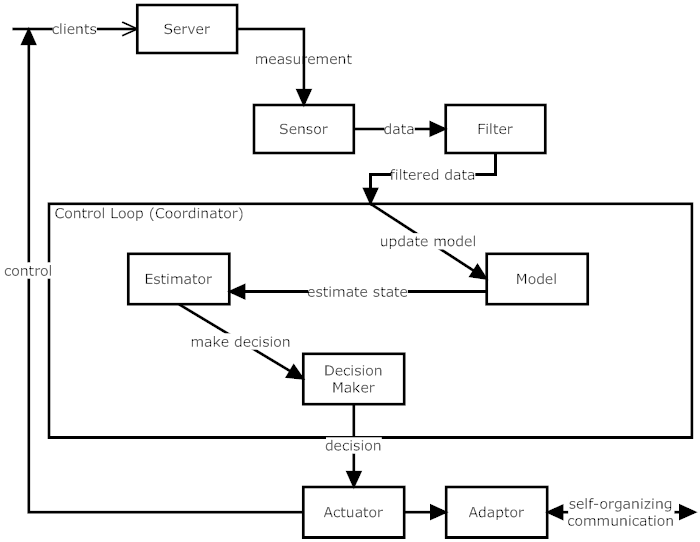
\includegraphics[width=0.9\linewidth]{Self-optimizingControlLoop_full}
	\caption{Self-Optimizing Control Loop Architecture}
	\label{fig:selfopt-archi}
\end{figure}

The fuzzy system will output a single metric representing the load of the server. This metric is then used by the self-organizing agents in order to predict an SLA breach and take actions to avoid the breach.

\section{SLA breach prediction: Ant Colony Optimization}

The ant colony optimization (ACO) algorithm \cite{antalgorithm}, \cite{selforg:aco} is best known for load balancing clouds or finding the best route in a network. The algorithm has received a lot of attention and work in academia and was presented in chapter \ref{Chapter_related}. At a high level the algorithm uses a number of simple agents called ants which traverse the network and leave a trail of pheromones which other ants can then follow. Good paths or solutions are reinforced by having more ants traverse them and leaving more pheromones. Once a path or solution is no longer viable, less ants travel it and another path is reinforced as more ants travel that path. In networking optimization ants behave as normal packets and traverse the network from router to router. When an ant reaches a router it can look at how long the arrival router's buffer queue is for the router the ant came from and then reinforce that route based on latency, buffer sizes, etc.

Take as an example a network that looks like the one in Figure \ref{fig:aco_init} in its initial non-traversed state, where the load of the links is the value shown on the edges of the graph, and in which ants start at node \textit{S} and finish at node \textit{E}. If there are 6 ants in the system, each ant deposits pheromone at a rate of $\frac{1}{edgeLoad}$, and in the initial state ants have an equal chance of taking an edge as there are no pheromones deposited, then the initial probability of an ant taking any given edge is shown in figure \ref{fig:aco_initprob}. Each edge in figure \ref{fig:aco_initprob} has a probability of being traversed by an ant of $\frac{1}{numberEdgesFromNode}$.

After the first run of the ants the pheromone in the network will look as in figure \ref{fig:aco_pher}. In figure \ref{fig:aco_pher} the edges show the number of ants taking each edge and the total amount of pheromone deposited in the form of $\frac{numberAnts}{totalPheomoneLevel}$. For example, the edge from \textit{S} to \textit{1} has 2 ants traversing it and total pheromone being deposited with a value of 2, while the edge from \textit{5} to \textit{6} has 2 ants traversing it and total pheromone being deposited with a value of 4 because the link has less load. While this example assumes that the ants split exactly as the probabilities shown in figure \ref{fig:aco_initprob}, note that it possible for more ants to take an edge with lower probability since ants roll a random value when deciding the edge to take.

When going back to the source, more ants will prefer edges with higher pheromone values thus resulting in that path being reinforced as shown in figure \ref{fig:aco_finalprob} where the probability of ants taking an edge is shown. This example does not include the decay of the pheromone level, but in an ACO implementation the pheromone level always decays at a given rate such that edges that are no longer traveled have their pheromone levels slowly decrease. As more time passes, ants will continue to add more pheromone on good paths in the end resulting in the path with the lowest load being reinforced. If the load in the network changes, ants will be able to start reinforcing the path with the better performance and forget about the previous path.

\begin{figure}
	\centering
	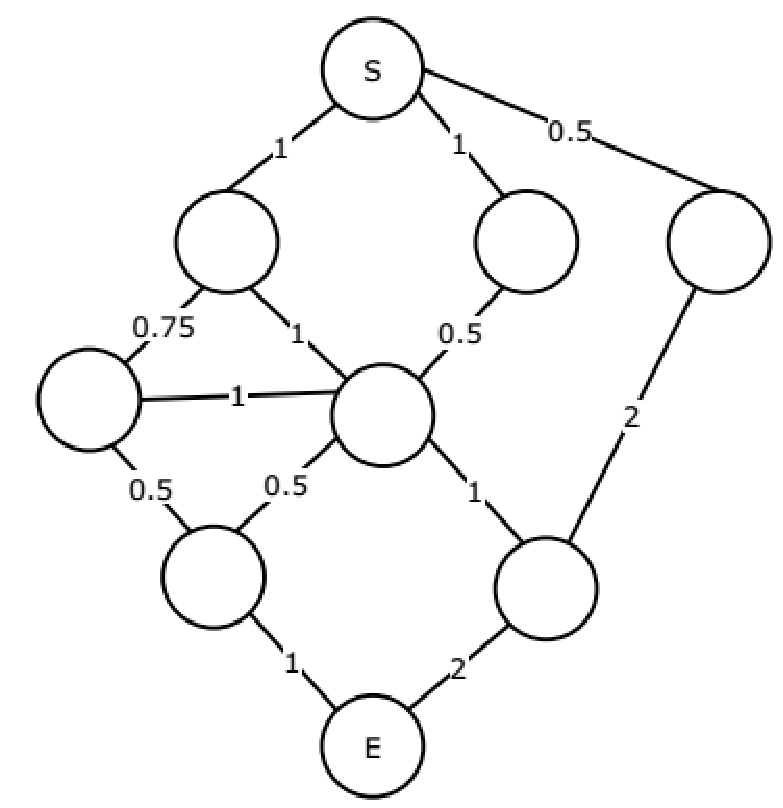
\includegraphics[width=0.9\linewidth]{aco_init}
	\caption{Network Ant Colony Optimization - Initial state}
	\label{fig:aco_init}
\end{figure}

\begin{figure}
	\centering
	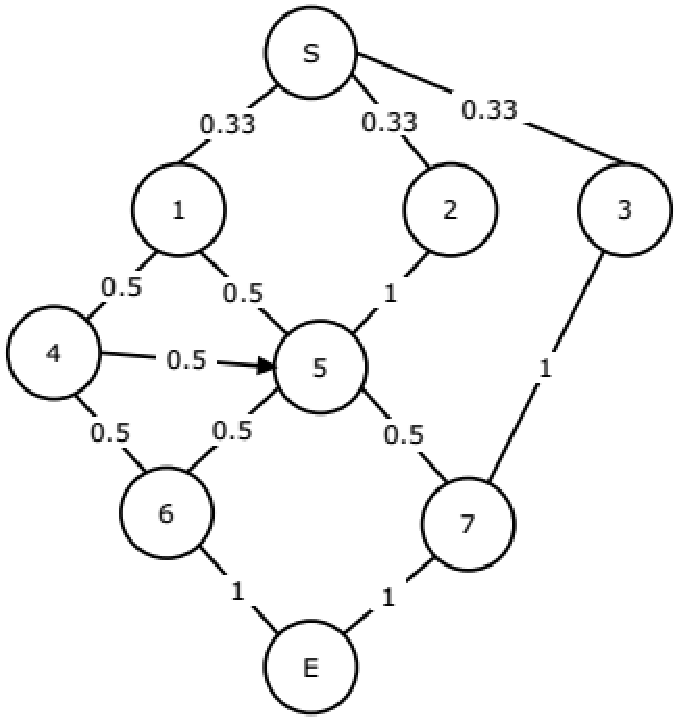
\includegraphics[width=0.9\linewidth]{aco_initprob}
	\caption{Network Ant Colony Optimization - Path probability initial}
	\label{fig:aco_initprob}
\end{figure}

\begin{figure}
	\centering
	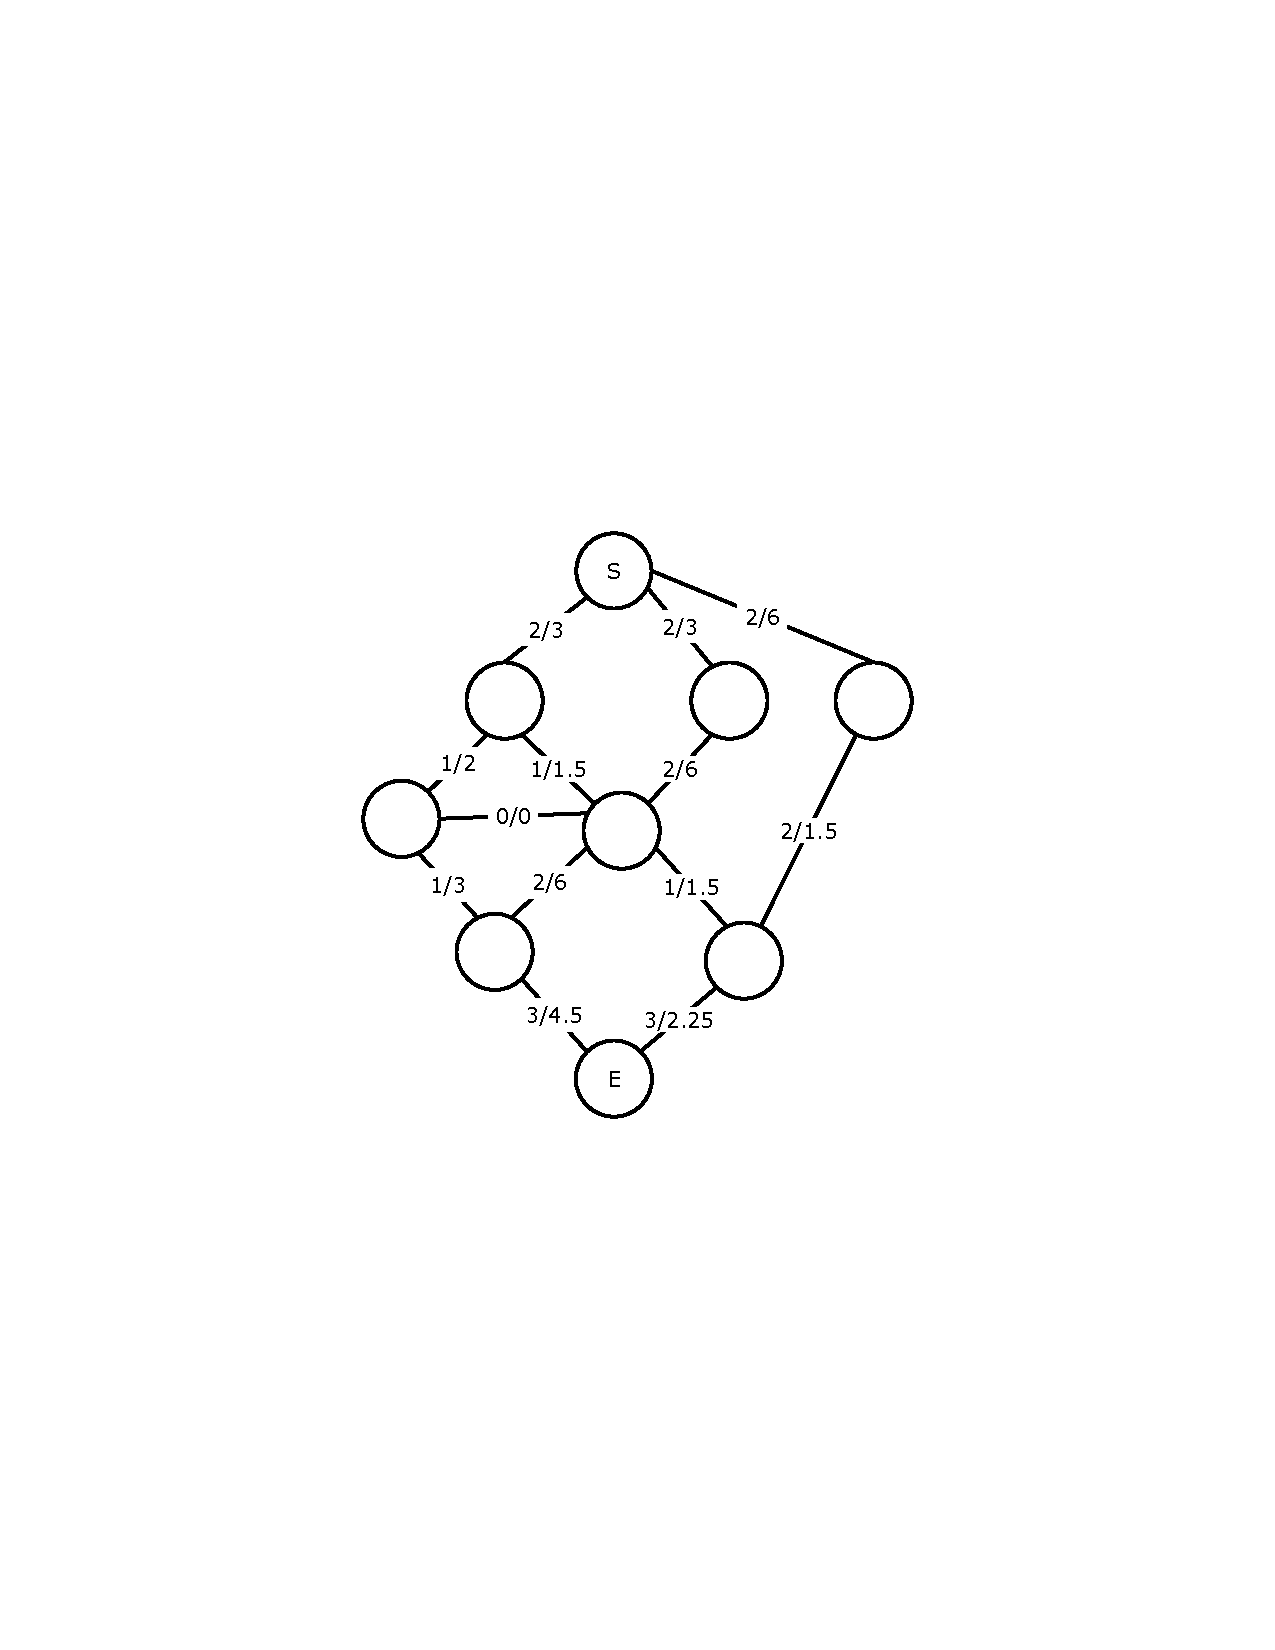
\includegraphics[width=0.9\linewidth]{aco_pher}
	\caption{Network Ant Colony Optimization - Pheromone update}
	\label{fig:aco_pher}
\end{figure}

\begin{figure}
	\centering
	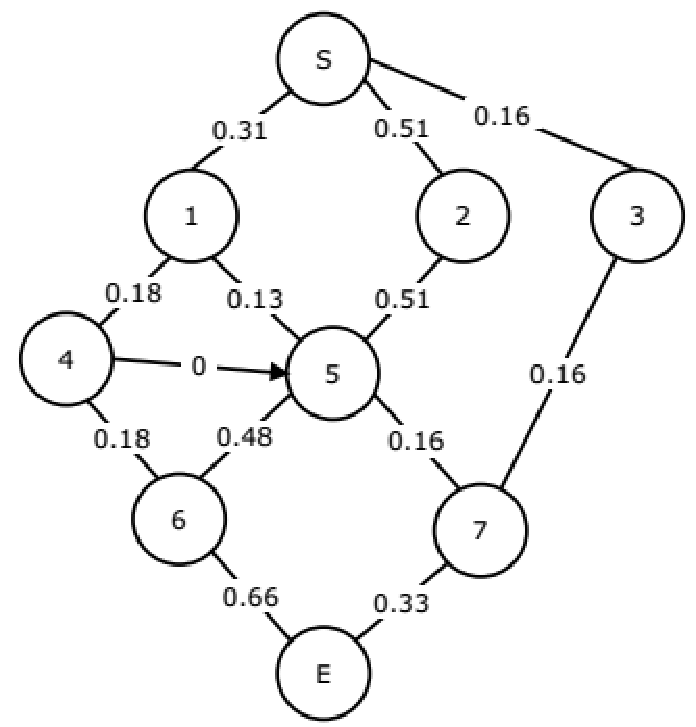
\includegraphics[width=0.9\linewidth]{aco_finalprob}
	\caption{Network Ant Colony Optimization - Path probability update}
	\label{fig:aco_finalprob}
\end{figure}

\subsection{ACO Model for SLA breach prediction}

The self-organizing algorithm used to predict SLA breaches in cloud systems is similar in nature to how the ACO algorithm behaves when finding the best route in a network. However, there are a number of significant differences due to the nature of the problem that is being resolved. The goal of the ACO algorithm while performing path optimization is to discover how viable different routes are and reinforce the good routes while at the same time diminishing the use of bad routes. For this problem the ants deposit pheromones on the routes between nodes such that paths with higher pheromones are more desired. In the case of the SLA breach prediction problem, the goal of the ACO algorithm is to determine based on the knowledge about the visited servers if the whole cloud is about to breach it's SLA requirements. For this problem, the ants deposit pheromones at the servers and use the amount of pheromone as a proxy of how loaded the whole cloud.

The ACO model for SLA breach prediction is composed of three components:

\begin{enumerate}
	\item Ants - ants are simple agents which traverse the network of servers and deposit pheromone at the servers based on a mathematical model
	\item Pheromone levels - each server has it's own pheromone level which is increased by ants visiting the server and decays periodically. Pheromones are a proxy of how overloaded a single server is.
	\item Mathematical model - this is the model which converts the fuzzy model result of each server into a pheromone value. The mathematical model also represents when an SLA breach is predicted.
\end{enumerate}

\subsection{Self-organizing agent: The ant}

Ants are simple agents that traverse the network of servers. They have no knowledge about the global state of the cloud and how overloaded all the servers in the cloud are. Ants only know the state at the currently visited server and also have a short memory about the last $x$ servers which the ant has visited and what the pheromone level was at those servers.

Whenever a server starts, the server's control system creates a new ant and sends it through the network of servers. Thus the total number of ants is equal to $N$ where $N$ is the number of live servers in the cloud. When an ant is first created, because it has no prior knowledge, it is sent to another server randomly. If only one server exists in the cloud, then the ant keeps visiting the same server.

As ants reach other servers they deposit pheromone at the server they arrive at, at a rate inversely proportional to the load of the server as represented by the fuzzy control system. At the same time ants wait at the server a time proportional to the load of the server. Thus overloaded servers will have less pheromone deposited when compared to an under-loaded server. By having ants wait a longer time at overloaded servers, the overall amount of pheromone in the network will further decrease. With this approach, a lower average amount of pheromone in the network of servers means that the cloud has higher load due to the fact that a larger number of servers have low pheromone levels because of being overloaded.

Ants also store information about the last $x$ servers the ant has visited and the time passed since the last visit to each of these servers. When an ant decides which server to go to, it uses a random function which is proportional to the time since it has visited a server combined with the pheromone level of the destination server. Thus the ant will give preference to the servers it has not visited in a long time, and especially the servers it has never visited or which are not in it's memory. Because the server structure is not stable and servers can join and leave at any time, ants decide the next server to visit based on the servers known by the current server the ant is at.  Assume a cloud with 5 servers and an ant which has the information in table \ref{tab:ant_prio} in it's history table and which reaches Server 5.

\begin{table}
\centering
\begin{tabular}{c|c|c}
Server & Time since last visit (s) & Pheromone Level \\
Server 1 & 15 & 10 \\ 
Server 2 & 20 & 5 \\
Server 3 & 5 & 8 \\
Server 4 & 35 & 5.5 \\
Server 5 & 0 & 10 \\
\end{tabular}
\caption{Ant routing knowledge prior}
\label{tab:ant_prio}
\end{table}

Based on the table, the ant computes the probability of visiting each server as:

\begin{equation}
P_s = (t_s / \sum_{i=1}^{N} t_i + p_{s} / \sum_{i=1}^{N} p_i) / 2
\end{equation}

where $P_s$ is the probability of visiting server $s$, $t_s$ is the time since it has visited server $s$ last time and $p_{s}$ is the pheromone at server $s$. These probabilities are computed only on the servers known as being up by the server the ant is at. The server the ant is currently at has to be excluded from the calculations, and it's visit probability will be 0. Assuming also that Server 5, which is the server the ant is at currently does not yet know about server 3. As such, the visit probability table looks as in Table \ref{tab:ant_prob}.

\begin{table}
\centering
\begin{tabular}{c|c}
Server & Probability (\%) \\
Server 1 & 35.10 \\
Server 2 & 26.48 \\
Server 4 & 38.42 \\
Server 5 & 0 \\
\end{tabular}
\caption{Ant routing probability}
\label{tab:ant_prob}
\end{table}

As such, the ant will roll a random value between 0 and 1, and choose which server to go to. A value between 0 and 0.3842 means that the next server will be \textit{Server 4}, between 0.3842 and 0.7352 it means that the next server will be \textit{Server 1} and a value between 0.7352 and 1 means \textit{Server 2}. Assuming the random value the ant rolls is 0.7, and that the ant waits at Server 5 for 5s and deposits 1 pheromone, the routing table after the ant moves to the next server will be as the one in Table \ref{tab:ant_post}.

\begin{table}
\centering
\begin{tabular}{c|c|c}
Server & Time since last visit (s) & Pheromone Level \\
Server 1 & 0 & 10 \\
Server 2 & 25 & 5 \\
Server 3 & 10 & 8 \\
Server 4 & 40 & 5.5 \\
Server 5 & 5 & 11 \\
\end{tabular}
\caption{Ant routing knowledge posterior}
\label{tab:ant_post}
\end{table}

In order to avoid having all ants visit a new node at the same time, whenever an ant discovers a new server it initializes the time since it visited the server with a random value. Assume that after the ant reaches Server 1, it discovers a new server which was unknown before - Server 6. The time since last visiting Server 6 will be initialized with a random value between 0 and the maximum time since last visiting a server which is known to be alive as in Equation \ref{eq:randomnew}. Furthermore the known pheromone level of the new server will be 0. If Server 1 only knows Server 2, 3 and 5 then the random value will be between 0 and 25s.

\begin{equation}
t_{new} = random(0, max(t_{known}))
\label{eq:randomnew}
\end{equation}

An ant's behaviour can be described by the algorithm below:

\begin{algorithm}
\begin{algorithmic}
	\State Calculate pheromone at current node
	\State Update ant's server history tables
	\If{Ant should morph}
		\State Morph ant
	\Else
		\State Calculate next server for ant
		\State Send ant to next server
	\EndIf
\end{algorithmic}
\caption{Ant Colony Optimization Pseudocode}\label{ant:pseudocode}
\end{algorithm}

For example, for a network of five servers Figure \ref{fig:antnetwork} shows the behaviour of the ant algorithm.

\begin{figure}
	\centering
	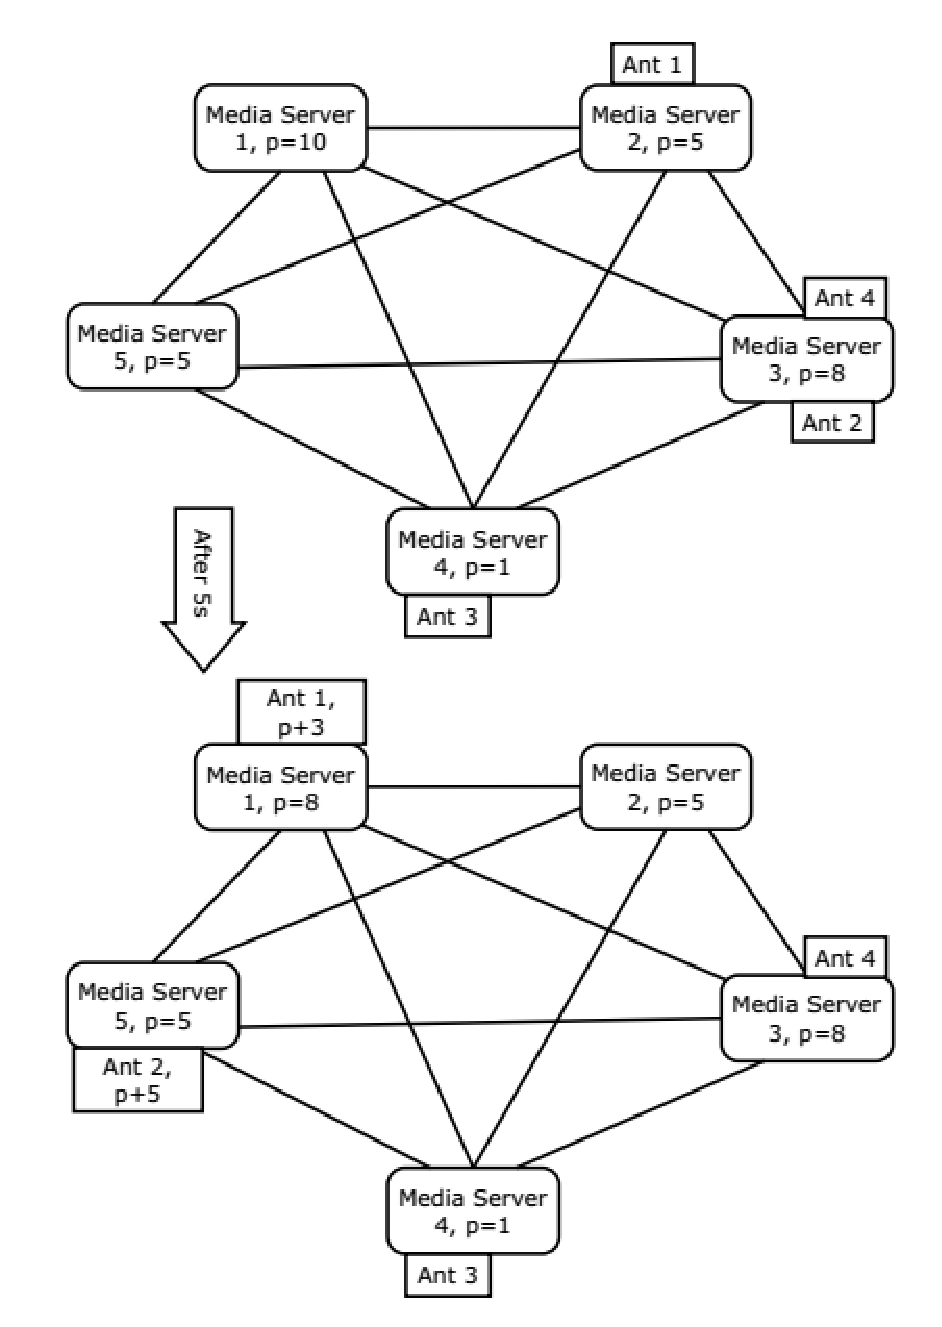
\includegraphics[width=0.9\linewidth]{aco_cloud}
	\caption{Ant Colony Optimization Network}
	\label{fig:antnetwork}
\end{figure}

\subsection{Server and cloud load: Pheromone levels}

For the purpose of controlling the number of servers in the cloud, the pheromone level in the network is used as a proxy for how loaded the entire cloud of servers is and is used to decide when to add or remove servers. As ants move through the network of servers they deposit pheromones - whenever an ant reaches a server it computes how much pheromone to deposit based on the result of the control system for that server. If the server's control system has a result which shows that the server is underloaded then more pheromone is deposited. If the server is overloaded then less pheromone is deposited. At the same time the pheromone amount at each server decays periodically at a constant rate. As such, a large amount of pheromone shows that servers are underloaded and servers should be removed, while a small amount of pheromone shows that servers are overloaded and that servers should be added.

For example, assume that an ant $k_{1}$ deposits an amount of pheromone $\tau_{k1}$ when it reaches a node which has 0 load - represented by a high fuzzy confidence value, and waits at an under-loaded node $15s$. Another ant $k_{2}$ which reaches a node where the confidence value is $50\%$ of the higher threshold will deposit only $\tau_{k} * (1 - p)$ where $p$ is the fuzzy confidence as a percentage and waits at the node a time of $15s/(1-p)$ with a maximum wait time of $60s$ to avoid waiting an infinite time when $p$ approaches $100\%$. At the same time, the pheromone left by the ants decays at a rate of $\rho$ every $15s$. As such, the amount of pheromone at any node can be seen as:

\begin{equation}
p^{t}_{n} = p^{t-1}_{n} + \sum_{i=1}^{K}(\tau * (1 - p)) - \rho
\end{equation}

where $p^{t}_{n}$ is the amount of pheromone at node $n$ at time $t$ where $t$ can be considered discrete in $15s$ increments and $K$ is the amount of ants arriving at the node in the time frame between $t-1$ and $t$.

On top of updating the pheromone at each server, each ant is also responsible for measuring the pheromone level at each node it visits. Ants store a history of the last $x$ nodes that they visited and the pheromone level at each of these nodes. Every time an ant moves to a new server, it removes the oldest pheromone value from this list and adds the pheromone at the current node. It then computes an aggregate metric of the pheromone at the last $x$ nodes visited, which is a simple average:

\begin{equation}
p_{ant} = \sum_{i=1}^{N} p_{N} / N
\end{equation}

where $p_{N}$ is the pheromone at server $N$. Once the pheromone level of an ant goes under a predefined value, the ant triggers the algorithm to determine the new count of servers which should be added to the cloud. Similarly, if the pheromone level of an ant becomes too high, the ant triggers the algorithm to determine the number of servers which should be removed from the cloud. The algorithm used to increase or decrease the size of the cloud triggers when more than half of the ants in the system agree that the algorithm should start. Until enough ants agree to start the cloud size optimization the ants continue moving through the network of servers and update the pheromone levels. Once more than half of the ants agree all ants stop and the optimization algorithm starts.

\subsection{Mathematical model}

The pheromone level at a single node is defined as mentioned in the previous section as:

\begin{equation}
p^{t}_{n} = p^{t-1}_{n} + \sum_{i=1}^{K}(\tau * (1 - p)) - \rho
\end{equation}

where $p^{t}_{n}$ is the amount of pheromone at node $n$ at time $t$ where $t$ can be considered discrete in some time increment and $K$ is the amount of ants arriving at the node in the time frame between $t-1$ and $t$.

There are a number of parameters that are used in order to tune the ACO algorithm:

\begin{enumerate}
	\item Decay amount - the amount that the pheromone level decreases at each server: $\rho$
	\item Decay rate - how often does the pheromone level decay at each server: $T_{decay}$
	\item Ant wait time - the minimum wait time for an ant at a server: $T_{minwait}$
	\item Ant pheromone level - the maximum amount of pheromone deposited by an ant at a server: $\tau_{max}$
	\item Ant history size - how many servers an ant should store in it's history
	\item Minimum/maximum morph level - the minimum/maximum pheromone level across the last $x$ servers visited by the ant required for the ant to morph: $Pt_{max}$/$Pt_{min}$
\end{enumerate}

\subsubsection{Under-loaded server}

If an under-loaded server is considered where the ant waits the minimum time and deposits the maximum amount of pheromone and we set $T_{decay} = T_{minwait}$ then in each time period the amount of pheromone at the server can be defined as:

\begin{equation}
\begin{aligned}
p^{t}_{n} &= p^{t-1}_{n} + (\tau_{max} - \rho) \\
p^{t}_{n} &= (n - 1) * (\tau_{max} - \rho)
\end{aligned}
\end{equation}

At the same time the ant will make a decision when $p^{t}_{n} > Pt_{max}$ or $p^{t}_{n} < Pt_{min}$. Because the server is under-loaded we expect that the amount of pheromone will continuously increase since the ant's goal should be to remove servers due to over-provisioning. The ant will make a decision when:

\begin{equation}
\begin{aligned}
p^{t}_{n} &= Pt_{max} \\
(n - 1) * (\tau_{max} - \rho) &= Pt_{max} \\
(n - 1) &= \frac{Pt_{max}}{(\tau_{max} - \rho)} 
\end{aligned}
\end{equation}

As such it can be determined that:

\begin{enumerate}
	\item $\tau_{max}$ must be greater than $\rho$
	\item The time to wait before the ant makes a decision can be defined by $Pt_{max}$ and $(\tau_{max} - \rho)$. A smaller difference between $\tau_{max}$ and $\rho$ will lead to slower decisions, while a smaller $Pt_{max}$ will lead to quicker decisions.
\end{enumerate}

\subsubsection{Balanced server}

If a balanced server is considered - that is a server where the fuzzy function shows that the server is well balanced and neither under-loaded, nor overloaded then both the amount of pheromone and the wait time of the ant change. Define $T_{b}$ as the time for the ant to wait at a balanced server and $\tau_{b}$ as the amount of pheromone deposited at a balanced server. Both $T_{b}$ and $\tau_{b}$ are defined in terms of the fuzzy function, where $T_{b} = T_{minwait} / (1 - p)$ and $\tau_{b} = \tau_{max} * (1 - p)$

\begin{equation}
\begin{aligned}
p^{t}_{n} &= \frac{t *  \tau_{b}}{T_{b}} - \frac{t *  \rho}{T_{decay}} \\
p^{t}_{n} &= \frac{t *  \tau_{max}(1 - p)}{\frac{T_{minwait}}{1 - p}} - \frac{t *  \rho}{T_{decay}}
\end{aligned}
\end{equation}

The goal of the ant system in such a case is to maintain the level of the pheromone such that servers are not added or removed. As such it can be determined that:

\begin{equation}
\frac{t *  \tau_{max}(1 - p)}{\frac{T_{minwait}}{1 - p}} = \frac{t *  \rho}{T_{decay}}
\end{equation}

which means that the amount of decay equals the amount of pheromone deposited over long periods of time.

\begin{equation}
\begin{aligned}
t *  \tau_{max} * (1 - p) * T_{decay} &= t *  \rho * \frac{T_{minwait}}{1 - p} \\
\tau_{max} * (1 - p)^2 * T_{decay} &= \rho * T_{minwait} \\
\frac{\tau_{max} * (1 - p)^2}{\rho} &= \frac{T_{minwait}}{T_{decay}}
\end{aligned}
\end{equation}

If as in the previous case for an under-loaded server $T_{minwait} = T_{decay}$, then the equation becomes:

\begin{equation}
\begin{aligned}
\tau_{max} * (1 - p)^2 &= \rho
\end{aligned}
\end{equation}

This equation allows the user to set the relation between $\tau_{max}$ and $\rho$ for a given $p$ where the cluster size should be stable. For example, if a cluster size should be stable when $p = 50\%$ then

\begin{equation}
\begin{aligned}
\tau_{max} * (0.5)^2 &= \rho \\
\tau_{max} * 0.25 &= \rho
\end{aligned}
\end{equation}

\subsubsection{Over-loaded server}

The previous equation holds for an over-loaded server as well. If we take the same example as before where the system is set to be balanced for $p = 50\%$, if $p$ goes up to $90\%$ then the previous equation becomes:

\begin{equation}
\begin{aligned}
p^{t}_{n} &= \frac{t *  \frac{\rho}{0.25} * 0.1}{\frac{T_{decay}}{0.1}} - \frac{t *  \rho}{T_{decay}} \\
p^{t}_{n} &= \frac{t *  \frac{\rho}{0.25} * 0.1}{\frac{T_{decay}}{0.1}} - \frac{t *  \rho}{T_{decay}} \\
p^{t}_{n} &= \frac{t * \rho}{T_{decay}} * (0.04 - 1) \\
p^{t}_{n} &= \frac{t * \rho}{T_{decay}} * -0.96
\end{aligned}
\end{equation}

This equation means that the pheromone rate at the node will decrease by $\rho * -0.96$ every decay period.

\subsection{Cluster optimization: Ant house hunting}

The ant house hunting algorithm can be used in order to optimize the number of servers in the cloud by having ants search for the optimal number of servers which should be up in the cloud. This algorithm works by having each ant search for a new nest, where a nest is represented by a new optimum number of servers in the cloud. The algorithm assumes that there is a home nest where the ants can meet after searching for a new nest. Once all the ants have agreed on the same optimum value, the servers are added or removed as desired and all ants are morphed back into food foraging ants for the ACO algorithm. \cite{selforg:antreloc}

When an ant morphs into a house hunting ant it initializes itself with a possible solution for the new size of the cloud. These possible solutions are computed as permutations of the current size of the cloud as known by the server the ant is at. If the ant was morphed because of lack of pheromone, then the ant generates a random value which would represent the number of servers to be added. Each random value is proportional to the size of the cloud and the pheromone level across the last $N$ servers known by the ant. For example, if the cloud contains only 2 servers, then the ant is initialized with a random value between 1 and 2. However, if the cloud contains 100 servers, then the ant would be initialized with a random values, which is defined as:

\begin{equation}
ServerCount_{add} = 1 + rand * N / (p_{ant})
\end{equation}

such that the lower the pheromone value, the higher the probability of more servers being added. The random value has the effect of generating multiple possible solutions across different ants.

If however the ant was morphed because of too much pheromone, then it does a similar initialization, but in this case it randomly chooses $X$ servers and hides them from its knowledge of the cloud. The servers are still in the ant's history but it does not consider them for optimization calculations. Each ant will create a different such permutation of servers which are hidden.

The ant house hunting algorithm is performed in rounds and ants can be in one of four states:

\begin{enumerate}
	\item Search - This is the initial state of ants which search for a new nest
	\item Active - The ant is committed to a good nest and tries to recruit other ants to it
	\item Passive - The ant is committed to a bad nest and is waiting to be recruited
	\item Final - A single nest remains so all ants go to it and that is the solution
\end{enumerate}

The state diagram for the ants can be described as in Figure \ref{fig:anthousehuntingstate}

\begin{figure}
	\centering
	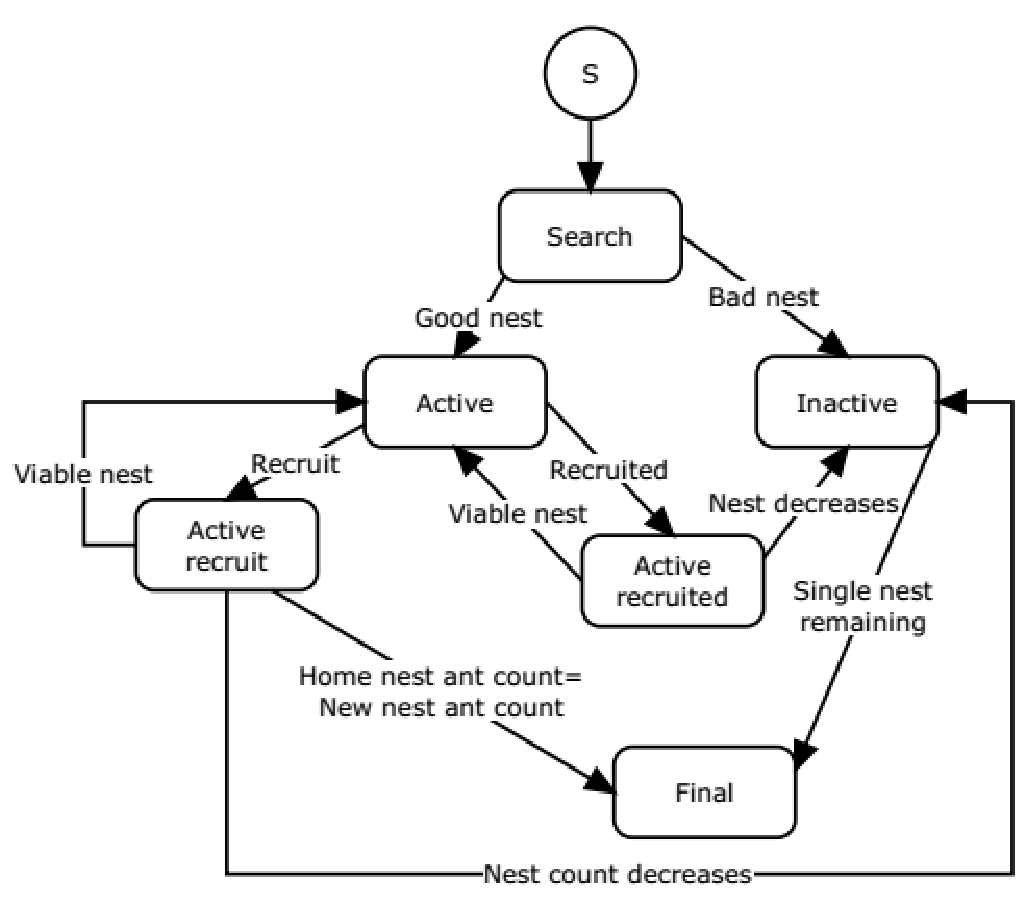
\includegraphics[width=0.9\linewidth]{aco_state}
	\caption{Ant House Hunting State Diagram}
	\label{fig:anthousehuntingstate}
\end{figure}

In the first round all house hunting ants search for a new nest by searching their solution space. This is achieved by having each ant choose one solution and simulating its effect on the pheromone level. If the ant is a server adder then the ant simulates that the $ServerCount_{add}$ servers are up and with no load. It picks $K$ servers from the list of the last $N$ servers it has visited and hides them, and replaces them with servers with no load. It then uses this information in order to simulate the pheromone level. If the ant is a subtractor, it hides $K$ servers where $K$ is defined as part of its random solution and simulates the effect this would have on its pheromone level. If the simulated result's performance is under a given threshold, then the ant goes into the passive state, otherwise it goes into the active state.

In the second round, all ants return home and active ants try to recruit other ants at the home nest. Passive ants can not be recruited until the final round when all ants go to the single remaining nest. Active ants recruit randomly from the other active ants at the home nest by choosing another ant to recruit and bring it to it's committed nest. In order to ensure no conflicts between recruiting ants, the ants recruit iteratively and an ant which was already recruited does not recruit someone else. Once an ants recruits another ant, then the two ants go together to the nest of the recruiting ant.

When reaching a new nest, active ants count the number of ants at the nest and check if the nest they reached is the same as the previous nest they went to. Based on the number of ants and the nest there are three cases:

\begin{enumerate}
	\item If the nest is the same nest that the ant went to before and the number of ants has increased or remained the same then the nest is still a possible solution so the ant updates the count and waits an extra round at the nest. After waiting a round, the ant checks if the number of ants at the home nest is the same as that at it's current nest. If they are the same then the ant goes to the final state, new servers are added or removed and all ants morph back to ACO ants.
	\item If the nest is the same nest that the ant went to before and the number of ants has decreased then the ant becomes passive because the nest is in the process of being dropped out, and returns home in the same round that active ants wait at the new nest.
	\item If the nest is different then the nest the ant was committed to then the ant waits a round and then it checks to see if the number of ants at it's new nest has decreased or not. If the number has decreased, then this nest is dropping out as the ants already committed to it have gone to the home nest and the ant becomes passive. Otherwise, the ant commits to it's new nest and goes home to recruit other ants.
\end{enumerate}

The above algorithm can be described as follows in pseudo-code in Figure \ref{ant:pseudocodeHouseHunting}. $R_{x}$ represents round x.

\begin{algorithm}
\begin{algorithmic}
	\State $R_{1}$: Go to new nest
	\State Compute suitability of new nest
	\If{Suitability $<$ threshold}
		Switch to passive
	\EndIf
	\State $R_{2}$: Go to home nest
	\If{Ant is active \&\& Ant is not recruited}
		\State Recruit another ant
		\State Go to new nest
	\ElsIf{Ant is recruited}
		\State Go to new nest
	\EndIf
	\State $R_{3}$: Count number of ants at new nest = $count_{new}$
	\If{Nest is same and $count_{new} >= count_{old}$}
		\State Wait round
	\ElsIf{Nest is same and $count_{new} < count_{old}$}
		\State Switch to passive
		\State Go to home nest
	\ElsIf{Nest is different}
		\State Wait round
	\EndIf
	\State $R_{4}$: Count number of ants at new nest $count_{new}$
	\If{$count_{new} == count_{home}$}
		\State Switch to final state
	\ElsIf{$count_{new} < count_{old}$}
		\State Switch to passive
		\State Go to $R_{2}$
	\EndIf
	\State Return final state
	\State Switch ants to ACO ants
\end{algorithmic}
\caption{Ant House Hunting Pseudocode}\label{ant:pseudocodeHouseHunting}
\end{algorithm}

\section{Self-organizing algorithm conclusions}

The proposed approach for the self-optimizing control of the geographically distributed multimedia cloud makes use of two self-organizing algorithms. The first algorithm is used in order to detect breaches of SLA before they happen such that proactive measures can be taken. The second self-organizing algorithm finds the optimal count of servers which should be running in the cloud.

The thesis uses the ACO algorithm to detect possible breaches of SLA by having ants continously move through the network and measure the load on the network of servers. This is a novel approach as previous reasearch has only focused on using the ACO to optimize various problems and not for detection of possible problems. The proposed approach ensures that the detection of SLA breaches can be done ahead of the actual breach while at the same time being fully scalabe as the self-organizing algorithm scales with the number of servers.

The second algorithm which optimizes the number of servers in the cloud makes use of a different self-organizing approach also inspired by the behaviour of ants. This algorithm is also novel as previous research into the house hunting algorithm was only used as a way to model the behaviour of ants and not for problem optimization.

The following chapter will introduce the test bed used to test the algorithms and also present results for the implementation of the self-optimizing self-organizing geographically distributed media cloud.
 % High Level design

\chapter{Performance tests for self-optimizing cloud} % Write in your own chapter title
\label{Chapter_testbed}
\lhead{Chapter \ref{Chapter_testbed}. \emph{Performance tests for self-optimizing cloud}} % Write in your own chapter title to set the page header

Two systems were used in order to test the performance of the self-organizing system previously described two systems were used. The first system is a collaborative application and a test bed which were developed and deployed to simulate a small cloud of servers. The second is a simulation environment developed using a well known simulation system for cloud systems - CloudSim \cite{related:cloudsim}. 

\section{Test-bed collaborative application}

An application was previously developed \cite{bogdan:miles2012chapter} in order to allow users to collaborate by sharing content and communicate via test and audio/video chat. The application is deployed using a Software as a Service model (SaaS) and has the following important characteristics:

\begin{enumerate}
	\item Server-client application - the system is a client-server application in which clients connect to a server and messages sent between clients go through the server, which distributes the messages to the appropriate destination clients.
	\item Cloud based application - clients connect to a cluster of servers which are virtualized, and clients communicating with each other could connect to different server instances in the cloud.
	\item Collaborative application - the system (servers in collaboration with the clients) ensures that clients in the same collaboration session view the same state of the shared ``workspace''. 
	\item Containerization - the servers are deployed in the cloud inside containers.
\end{enumerate}

and the following high level functional requirements:

\begin{description}
	\item[Client Presence] Clients can see when their contacts come online, go offline, join a collaborative session and become busy.
	\item[Client Synchronization] Clients in the same collaborative session must see the exact same thing in the collaborative part of the application.
	\item[Client Communication] Clients in the same session can communicate with each other via text, audio, video. 
	\item[Session Size] No restriction is set on how many clients in a session can broadcast video/audio at the same time.
	\item[Session Setup] Any user can invite another available user to a collaborative session (pending restrictions created by the session's controller). 
	\item[Session Number] Users can only participate in one session at any time.
	\item[Session Control] Either any user can choose what is viewed in the shared collaboration panel or the session's manager can restrict the control to himself only.
	\item[Session in Progress Synchronization] Clients who join a session already in progress must be synchronized to the state of the session.
\end{description}

One important property of the application is that users communicate with each other via video/audio chat while collaborating, and as such latency for the video streams is very important to manager in order to provide proper QoS to the users.

\section{Design and Implementation of a Test-Bed for the Self-Organizing Control of a Cloud Based Autonomic System}

A small test bed was created where various loads were applied to a cloud of media servers and the required data was measured from the servers. All servers are currently located in the same location on the same LAN and VLANs are used in order to separate servers into different logical networks. This is done in order to be able to simulate multiple datacenters (clouds) and be able to simulate network load on the connections between datacenters to test the geographically distributed cloud. Each of the hardware servers in the cluster run Docker \cite{cloud:docker}. Each docker container runs the Ubuntu OS and the required software for the container. A number of containers are used by the application:

\begin{enumerate}
	\item Media server container - users connect directly to these servers
	\item JGroups container for the communication between servers - servers communicate with each other via a JGroups GMS group in order to exchange client information
	\item Load balancer container for the cloud - users first connect to a load balancer which then redirects them to a server which will offer good QoS
	\item Self-organizing manager for a single media cloud container - each media server container has its own self-organizing manager
	\item Self-optimizing manager container for the cloud - a global manager which is responsible for adding/removing servers to/from the cloud
\end{enumerate}

Figure \ref{fig:deployment} shows the physical topology of the infrastructure, which will be used to simulate various deployment scenarios and run tests on how the collaborative system behaves. The test bed uses five servers connected via a switch to one of four routers with a fifth router providing outside internet connection. Figure \ref{fig:logicaldeploymentrouting} displays how routing will be done within the network and the various VLANs used to create the separate clouds. The server names are cloud1 through cloud5, with cloud4 and cloud5 being in the same VLAN, while cloud1, cloud2 and cloud3 are each in their own VLAN. The network connections are 100Mbps with some of the router connections being 10Mbps. While such connection speeds would be too low for a datacenter, it is fine for these tests as the low speeds can be used to simulate overloaded internet connections with low throughput.

\begin{figure}
	\centering
		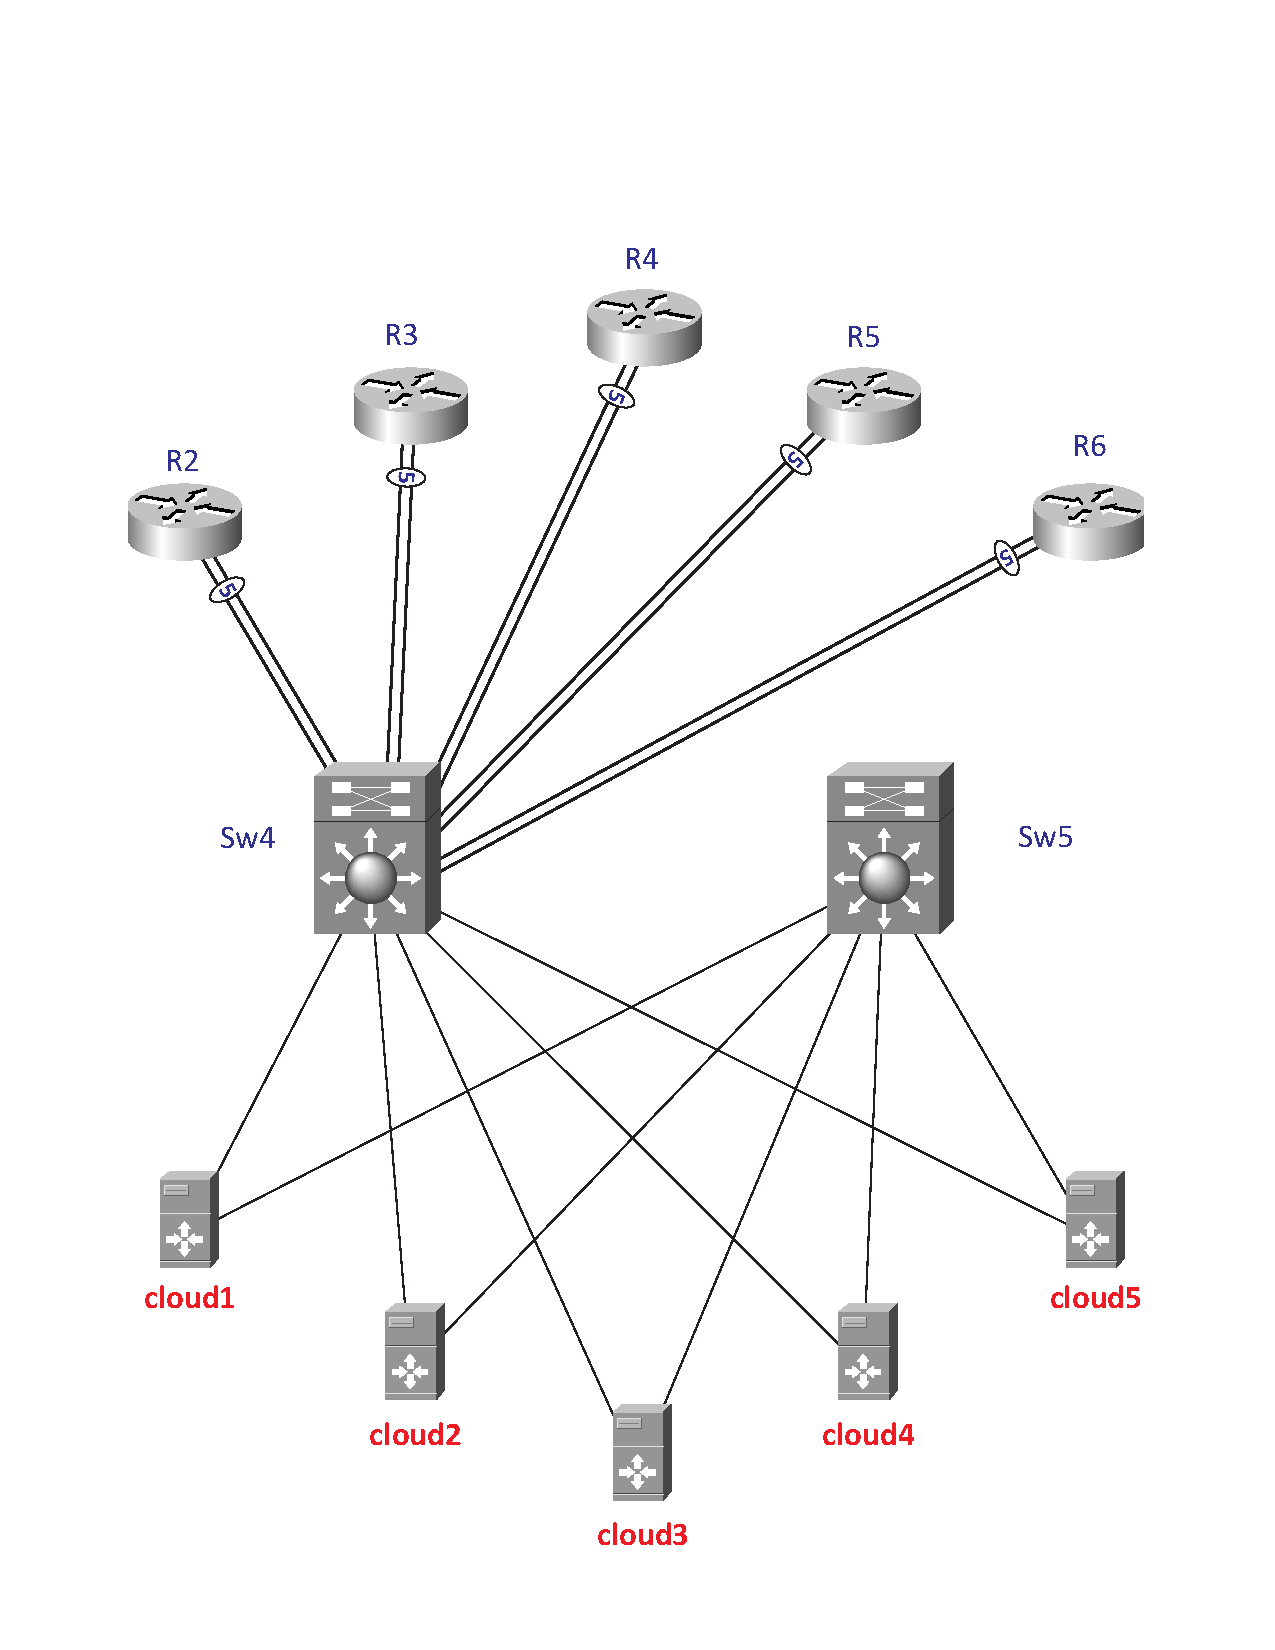
\includegraphics[width=\columnwidth]{01_physical_topology_v2_abstr}
	\caption{Physical Topology}
	\label{fig:deployment}
\end{figure}

\begin{figure}
	\centering
		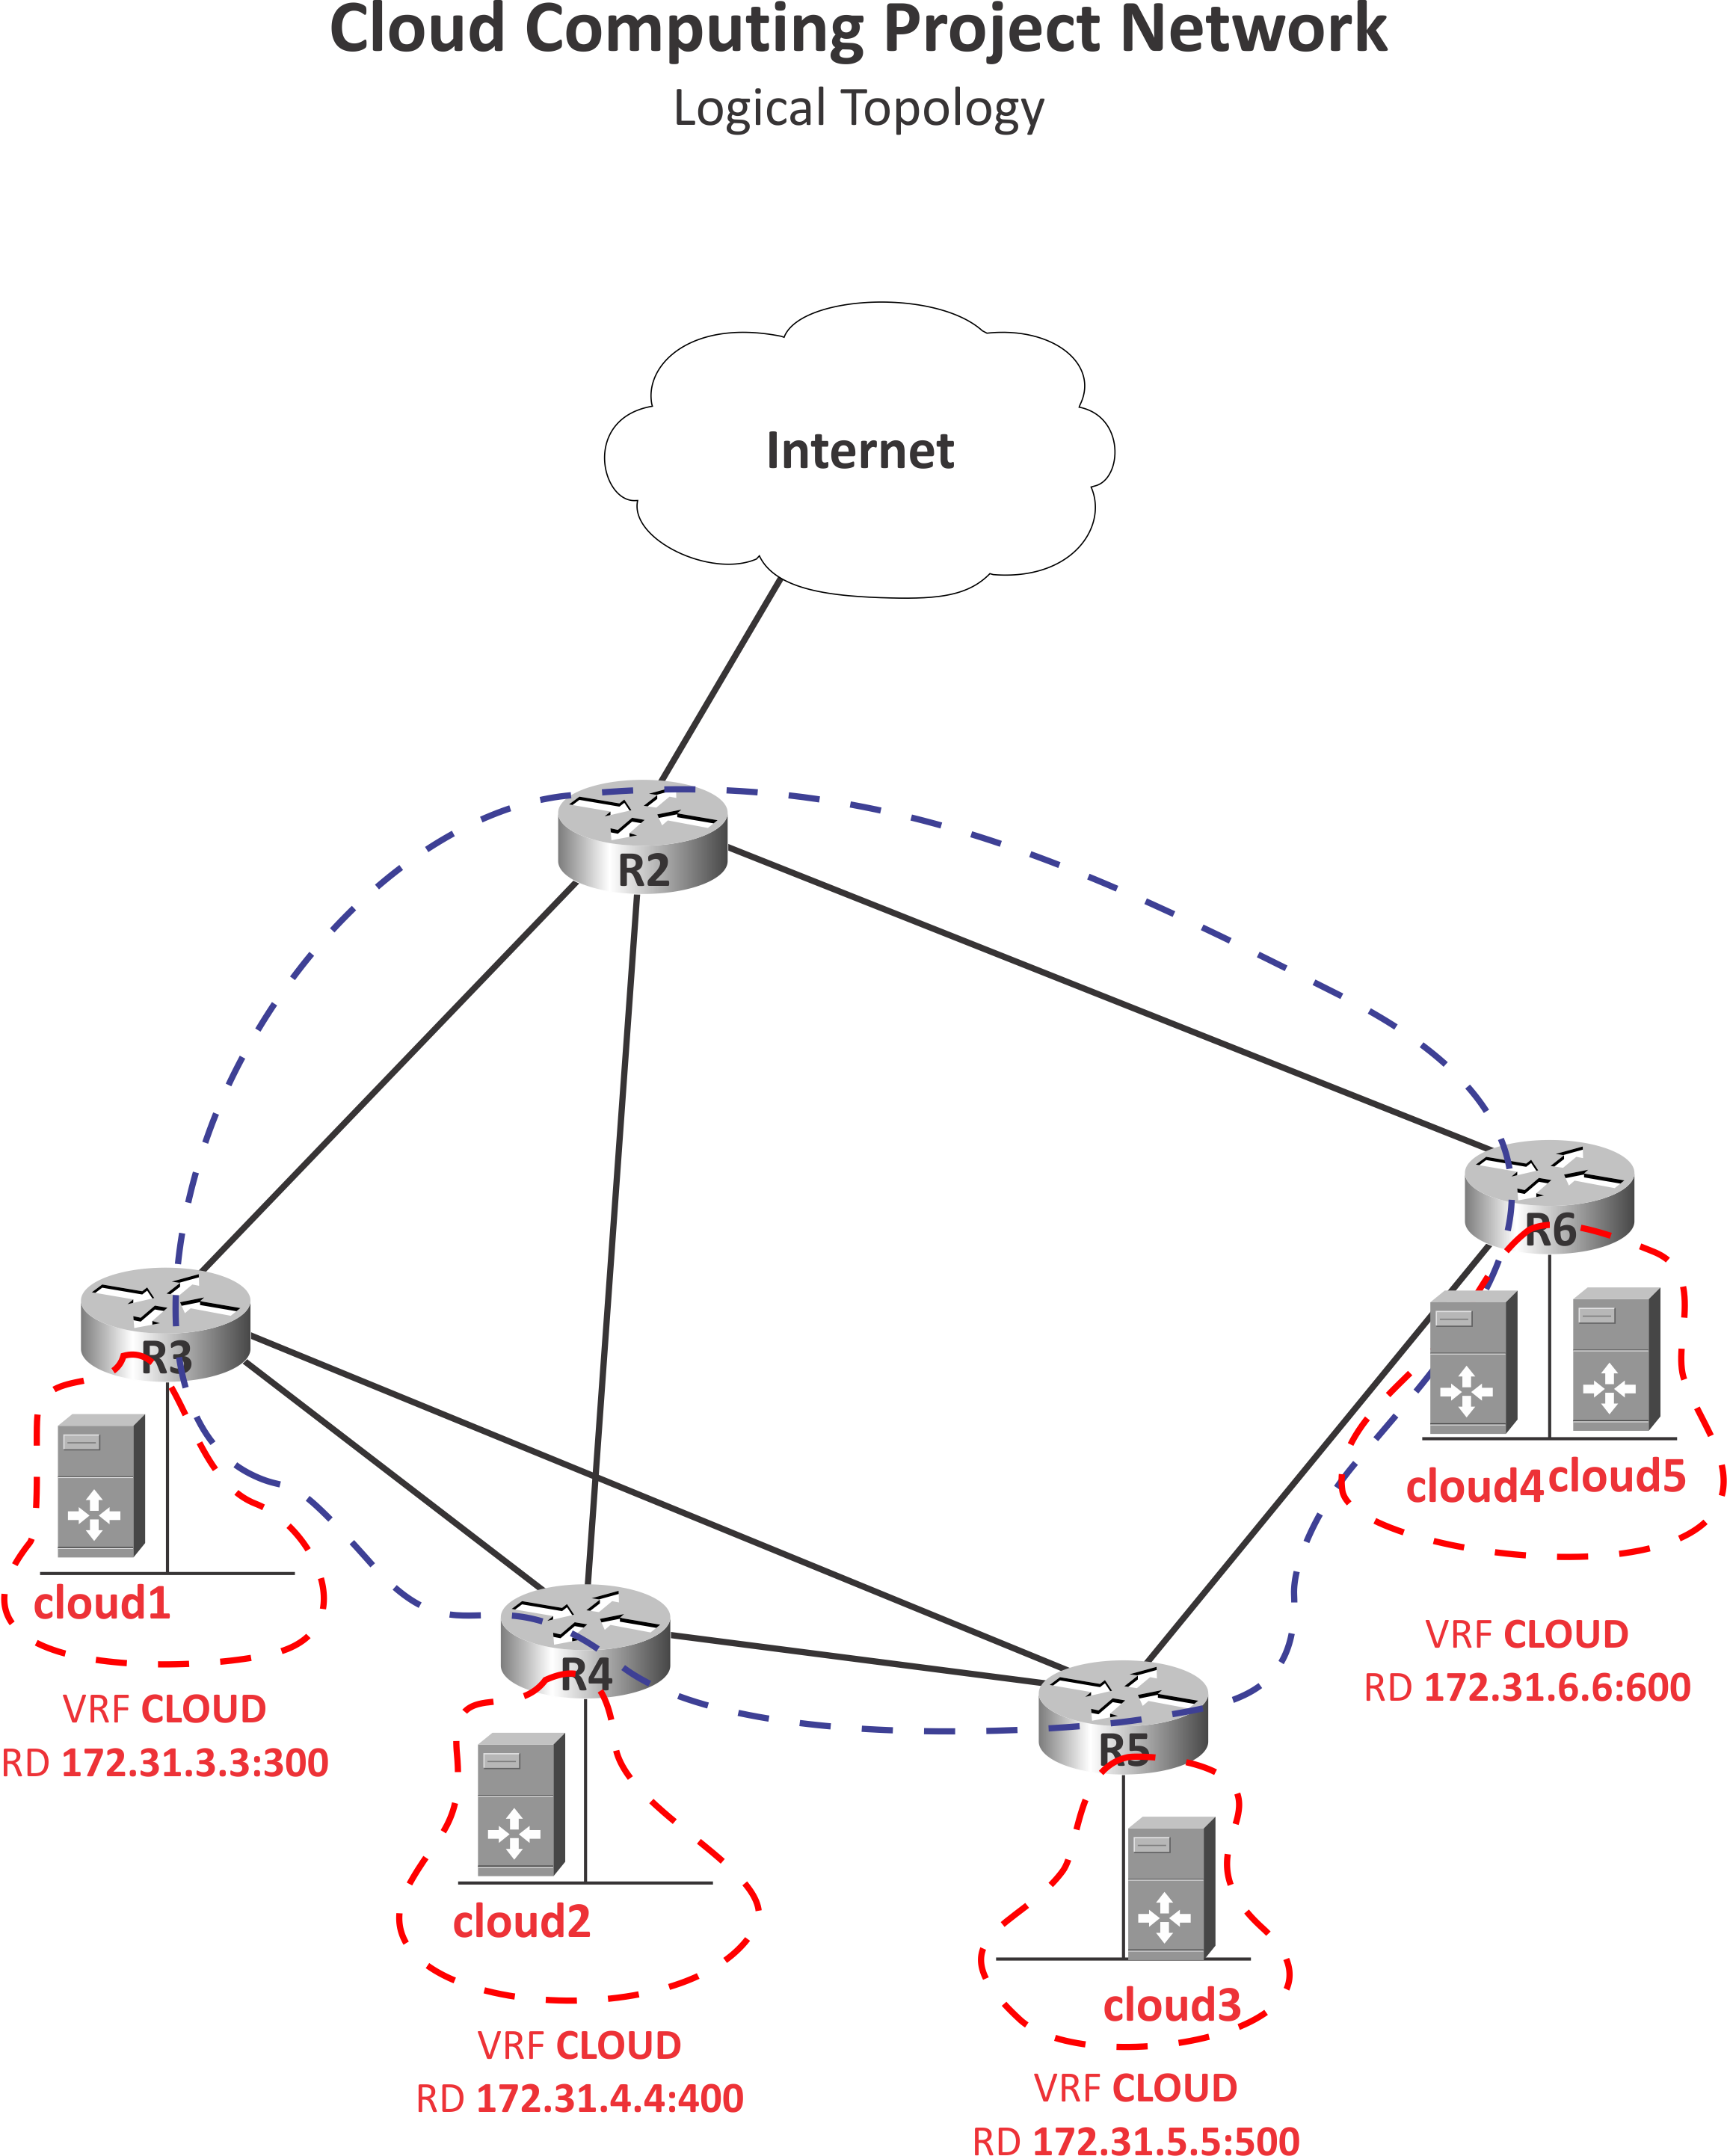
\includegraphics[width=\columnwidth]{05_logical_topology_routing_protocols_v2_abstr}
	\caption{Logical Topology Routing}
	\label{fig:logicaldeploymentrouting}
\end{figure}

A separate machine not shown in the diagrams is responsible for simulating client requests. In order to test audio/video streaming a prerecorded webcam video is streamed whenever the client simulator decides to start streaming. The stream used for testing is a 64x64 video stream at 25 frames per second with a bit rate of 180Kbps. The client simulator is written in Java and can simulate various client distributions by varying the amount of clients, the number of clients in every session, the number of clients streaming in each session and the time delay between messages being sent in a session. The simulator initially creates a number of sessions and a number of clients in each session. Each client is created with a given time to live. Periodically, the session calculates how many clients should be streaming in the session at that point in time. If more clients are required to stream than are currently streaming, the session simulator instructs a number of clients to start streaming also. If less clients are required to stream than are currently streaming, the session simulator instructs a number of clients to stop streaming. If there is no change in the number of clients needed to stream, then no change is made in which clients are streaming. Whenever a client reaches its time to live, the client is put to sleep and given a time after which it should wake up and reactivate. When a client reactivates it joins again the same session it was a member of, before going to sleep. The amount of time clients are awake and sleep is randomized thus generating various session sizes over time.

\subsection{System Behaviour Measurements}

First of all, using the test bed a number of runs were performed in order to determine the behaviour of the collaborative cloud. The tests vary one of four variables in order to determine how they affect the outputs of the media server clouds. For each of the tests presented in the following subsections one variable was modified while all others were kept constant. The four variables are the following:

\begin{enumerate}
	\item Number of servers in the cloud, varied from one to three.
	\item Number of collaborative sessions in each server, varied from one to six.
	\item Number of clients in each session, varied in increments of one from two to forty. In some cases, the increases in clients stopped before reaching the maximum due to the 10Mbps network link becoming saturated.
	\item Number of clients streaming per session, varied from one to four. 
\end{enumerate}

The tests presented here represent an exhaustive search of the variable space in order to determine how each of the four variables affects the system under test.

\subsection{Test Plan}

The data is measured from all the servers every 30 seconds, and is composed of: bandwidth received, bandwidth sent, latency and CPU usage. Since the tests are run at different moments in time, the timescale is normalized to the period from when each test was started.

The expectations are that as the number of servers increases for a given number of clients, sessions and streams the bandwidth and latency will decrease proportionally. Similar, as the number of collaborative sessions increases, with all other variables kept constant bandwidth and latency will decrease as the 1:N proportion, where N is how many clients receive the stream decreases. When the number of clients in a session increases bandwidth and latency should increase in a reverse fashion. Finally, when the number of streaming clients increases bandwidth and latency should increase similarly.

The graphs for the performance tests can be found online as they would take too much space here. In order to make the results more visible, the tests are grouped on the graphs 3 by 3, with the lowest test on one graph being the highest test on another graph. The following sections will present some of the results in tabular form and the rest of the results can be found online as well.

In order to simplify notations, test will be abbreviated in the form servers/sessions/incoming streams per session. For example, the test 3/1/4refers to a test with 3 servers, 1 session across all servers and 4 incoming streams from clients.

\subsubsection{1 Server, 1 Collaborative Session, 1 Stream Per Session}
\label{sec:1serv_1sess_1str}

The number of clients was varied from 2 to 40 in increments of 1. The number of outgoing streams is equal to (the number of users - 1) because the streaming user does not receive the stream back. These results show that as the number of users increases in a session, the latencies and CPU usage of the server increase at the same time. Interestingly mean CPU usage seems to reach an upper bound around 34 users while latencies continue to increase.

\subsubsection{1 Server, 1 Collaborative Session, 2 Streams Per Session}
\label{sec:1serv_1sess_2str180}

The number of clients was varied from 2 to 20 in increments of 1. The number of outgoing streams in this case will be equal to 2 * (the number of users - 1), as there are 2 streams going to all users in the session except the streamer. The pattern is similar to the previous case, with latencies and CPU usage increasing as the number of users in the session increases. Similar to before, CPU reaches a point where it peaks while latencies still increase. If similar numbers of outgoing streams were to be compared, it can be seen that the results are similar in both CPU usage and latency at lower number of users. For example, for 12 outgoing streams the previous test had a median CPU of 19.28 \% and median latency of 15.69 ms, while this test has a median CPU of 19.35 \% and median latency of 16.71ms. As the number of users increases however, the results of this test case are worse than the equivalent result of the previous test. For example, for 26 outgoing streams the previous test had a median CPU of 36.09 \% and median latency of 20.63 ms, while this test has a median CPU of 31.06 \% and median latency of 22.64 ms.

\subsubsection{1 Server, 1 Collaborative Session, 3 Streams Per Session}
\label{sec:1serv_1sess_3str180}

The number of clients was varied from 3 to 14 in increments of 1. The number of outgoing streams in this case will be equal to 3 * (the number of users - 1), as there are 3 streams going to all users in the session except the streamer. Like in the two previous cases CPU and latency increase as more users are added to the session. At similar levels of outgoing streams, the results for this test case are a bit worse than those of the two previous tests. For 12 outgoing streams, this results in a median latency of 20.41 ms, which is higher than 16.71 ms for the previous test and 15.69 ms for the first test.

\begin{table}
\caption{Median and Mean CPU, Latencies for 1 Server, 1 Session, 3 Stream}
\label{table:1serv_1sess_3str}
\begin{tabu} to\linewidth{|X[c]|X[c]|X[c]|X[c]|X[c]|X[c]|X[c]|X[c]|}
\everyrow{\hline}
\hline
Nr. of Users & Median Latency (ms) & Mean Latency (ms) & Median Message Latency (ms) & Mean Message Latency (ms) & Median CPU (\%) & Mean CPU (\%) & Out Stream Count\\
\taburowcolors 2{Gray!20..LimeGreen!50}
3 & 11.83 & 26.84 & 10 & 159.44 & 12.2 & 10.36 & 6 \\
4 & 11.75 & 23.48 & 10 & 22.25 & 16.49 & 14.38 & 9 \\
5 & 13.2 & 28.18 & 9 & 139.88 & 20.41 & 16.79 & 12 \\
6 & 17 & 22.06 & 10 & 53.82 & 20.04 & 16.42 & 15 \\
7 & 17.43 & 24.73 & 10 & 17.33 & 22.94 & 19.22 & 18 \\
8 & 16.25 & 28.08 & 10 & 32.48 & 26.24 & 22.29 & 21 \\
9 & 20.11 & 43.52 & 10 & 25.36 & 31.03 & 26.28 & 24 \\
10 & 19.3 & 31.01 & 11 & 53.42 & 34.48 & 29.43 & 27 \\
11 & 25.73 & 75.89 & 15 & 46.64 & 32.74 & 27.37 & 30 \\
12 & 30 & 67.83 & 15 & 45.34 & 35.04 & 29.77 & 33 \\
13 & 45.08 & 99.52 & 32 & 53.17 & 36.2 & 30.95 & 36 \\
14 & 76.82 & 112.76 & 34 & 39.84 & 39.52 & 34.06 & 39 \\
\end{tabu}
\end{table}

\subsubsection{1 Server, 1 Collaborative Session, 4 Streams Per Session}
\label{sec:1serv_1sess_4str180}

For this test, users were varied from 4 to 11 in increments of 1. Outgoing streams behave as previous and will be equal to 4 * (the number of outgoing streams). Same results as for the previous tests are observed, as median latency for 12 outgoing streams is even higher than the previous tests.

\begin{table}
\caption{Median and Mean CPU, Latencies for 1 Server, 1 Session, 4 Stream}
\label{table:1serv_1sess_4str}
\begin{tabu} to\linewidth{|X[c]|X[c]|X[c]|X[c]|X[c]|X[c]|X[c]|X[c]|}
\everyrow{\hline}
\hline
Nr. of Users & Median Latency (ms) & Mean Latency (ms) & Median Message Latency (ms) & Mean Message Latency (ms) & Median CPU (\%) & Mean CPU (\%) & Out Stream Count\\
\taburowcolors 2{Gray!20..LimeGreen!50}
4 & 11.88 & 17.23 & 10 & 14.55 & 21.59 & 18.1 & 12 \\
5 & 14.2 & 20.44 & 10 & 38.31 & 21.88 & 18.22 & 16 \\
6 & 18.33 & 26.47 & 11 & 37.45 & 27.19 & 22.72 & 20 \\
7 & 20.14 & 39.64 & 11.5 & 32.15 & 33.14 & 27.96 & 24 \\
8 & 22.62 & 49.37 & 13 & 26.71 & 35.71 & 30.28 & 28 \\
9 & 32.89 & 79.52 & 20.5 & 34.98 & 35.84 & 29.86 & 32 \\
10 & 30 & 82.61 & 24.5 & 54.45 & 37.32 & 31.55 & 36 \\
11 & 69.45 & 107.49 & 40 & 45.13 & 38.35 & 32.62 & 40 \\
\end{tabu}
\end{table}

\subsubsection{1 Server, 2 Collaborative Sessions, 1 Stream}
\label{sec:1serv_2sess_1str180}

In this test 2 collaborative sessions of equal size are created, but only one session contains a streaming client. In the second session, clients only exchange text/synchronization messages. The goal of this test is to determine if there are other factors in the application outside video/audio streaming impacting latencies and CPU usage. If this test was compared to the test in section \ref{sec:1serv_1sess_1str}, it would be expected that latencies are very similar for equal numbers of clients. This expectation is not met however, as similar numbers of users result in higher latencies for this test. CPU usage values are very close for all tests however. This suggests that first of all, latencies are not directly related to CPU usage, and at the same time that only the number of outgoing streams is not sufficient to determine the latency of the system.

\subsubsection{1 Server, 2 Collaborative Sessions, 4 Streams}
\label{sec:1serv_2sess_4str}

The same trend as before is shown by this test when compared to both the previous tests with 2 sessions and to the 1/1/4 test.

\begin{table}
\caption{Median and Mean CPU, Latencies for 1 Server, 2 Session, 4 Stream}
\label{table:1serv_2sess_4str}
\begin{tabu} to\linewidth{|X[c]|X[c]|X[c]|X[c]|X[c]|X[c]|X[c]|X[c]|}
\everyrow{\hline}
\hline
Nr. of Users/Session & Median Latency (ms) & Mean Latency (ms) & Median Message Latency (ms) & Mean Message Latency (ms) & Median CPU (\%) & Mean CPU (\%) & Out Stream Count\\
\taburowcolors 2{Gray!20..LimeGreen!50}
2 & 12.25 & 16.02 & 12 & 58.94 & 10.91 & 9.42 & 4 \\
3 & 16 & 24.18 & 12 & 20.44 & 16.75 & 13.7 & 8 \\
4 & 16.69 & 23.48 & 12 & 17.18 & 21.78 & 18.28 & 12 \\
5 & 16.25 & 27.37 & 11 & 52.32 & 22.55 & 19.18 & 16 \\
6 & 19.17 & 31.97 & 12 & 30.2 & 28.5 & 23.87 & 20 \\
7 & 22.79 & 49.1 & 12.5 & 33.83 & 31.85 & 26.27 & 24 \\
8 & 27.38 & 77.3 & 12.5 & 26.23 & 37.85 & 32.18 & 28 \\
9 & 45 & 77.44 & 20 & 35.24 & 36.82 & 31.38 & 32 \\
10 & 71.6 & 116.25 & 21 & 35.18 & 38.2 & 32.99 & 36 \\
\end{tabu}
\end{table}

\subsubsection{1 Server, 3 Collaborative Sessions, 3 Streams}
\label{sec:1serv_3sess_3str}

Comparing this test results with the results for 1 Server, 2 Collaborative Sessions, 3 Streams, for the same number of outgoing streams, CPU usage is very similar, while latencies are higher for this test. The reason for this, is that a similar number of outgoing streams for this case has more total users across the server.

\begin{table}
\caption{Median and Mean CPU, Latencies for 1 Server, 3 Session, 3 Stream}
\label{table:1serv_3sess_3str}
\begin{tabu} to\linewidth{|X[c]|X[c]|X[c]|X[c]|X[c]|X[c]|X[c]|X[c]|}
\everyrow{\hline}
\hline
Nr. of Users/Session & Median Latency (ms) & Mean Latency (ms) & Median Message Latency (ms) & Mean Message Latency (ms) & Median CPU (\%) & Mean CPU (\%) & Out Stream Count\\
\taburowcolors 2{Gray!20..LimeGreen!50}
2 & 14 & 19.06 & 11 & 16.43 & 8.3 & 7.43 & 3 \\
3 & 13.56 & 17.83 & 11 & 40.74 & 12.6 & 10.84 & 6 \\
4 & 16.17 & 18.44 & 11 & 28.72 & 16.86 & 14.9 & 9 \\
5 & 16.33 & 28.52 & 10 & 15.91 & 20.82 & 18.06 & 12 \\
6 & 19.89 & 28.45 & 11 & 18.02 & 20.84 & 17.52 & 15 \\
7 & 22.81 & 34.21 & 11 & 18.98 & 23.46 & 19.77 & 18 \\
8 & 20.9 & 38.72 & 11 & 21.45 & 29.21 & 24.71 & 21 \\
9 & 27.81 & 40.85 & 11 & 22.38 & 33.17 & 27.21 & 24 \\
10 & 35.65 & 73.61 & 11 & 26.09 & 35.04 & 29.64 & 27 \\
11 & 44.55 & 82.58 & 14.5 & 33.29 & 35.46 & 30.34 & 30 \\
12 & 40.06 & 111.62 & 15 & 31.79 & 38.11 & 31.4 & 33 \\
13 & 107.77 & 134.55 & 27.5 & 40.45 & 39 & 32.78 & 36 \\
14 & 71.73 & 126.28 & 18 & 31.79 & 39.02 & 28.9 & 39 \\
\end{tabu}
\end{table}

\subsubsection{2 Servers, 1 Collaborative Session, 3 Streams}

Comparing this test with the test for 1 Servers, 1 Collaborative Session, 3 Streams, the latency and CPU usage are similar for an equal number of outgoing streams. Doing the same comparison with the test for for 1 Server, 2 Collaborative Sessions, 3 Streams, the results are better for this result.

\begin{table}
\caption{Median and Mean CPU, Latencies for 2 Server, 1 Session, 3 Stream}
\label{table:2serv_1sess_3str}
\begin{tabu} to\linewidth{|X[c]|X[c]|X[c]|X[c]|X[c]|X[c]|X[c]|X[c]|}
\everyrow{\hline}
\hline
Nr. of Users/Server & Median Latency (ms) & Mean Latency (ms) & Median Message Latency (ms) & Mean Message Latency (ms) & Median CPU (\%) & Mean CPU (\%) & Out Stream Count\\
\taburowcolors 2{Gray!20..LimeGreen!50}
2 & 11 & 30.57 & 33 & 25.02 & 10.34 & 8.61 & 6 \\
3 & 14.33 & 22.17 & 32 & 24.33 & 13.46 & 11.44 & 9 \\
4 & 14.38 & 29.36 & 33.5 & 198.07 & 16.97 & 14.19 & 12 \\
5 & 15.2 & 20.99 & 35 & 86.81 & 19.98 & 16.18 & 15 \\
6 & 15.67 & 18.74 & 35 & 48.21 & 23.45 & 19.46 & 18 \\
7 & 19.14 & 36.61 & 36 & 33.92 & 26.53 & 22.04 & 21 \\
8 & 16.38 & 30.7 & 36 & 34.27 & 30.44 & 25.37 & 24 \\
9 & 19.22 & 38.75 & 37 & 39.36 & 33.24 & 26.62 & 27 \\
10 & 25.2 & 46 & 40.5 & 43.95 & 35.07 & 28.68 & 30 \\
11 & 21.45 & 59.71 & 45.5 & 104.72 & 36.31 & 29.23 & 33 \\
12 & 36 & 68.65 & 44 & 52.64 & 38.89 & 31.28 & 36 \\
13 & 62.77 & 91.37 & 60.5 & 69.6 & 40.33 & 33.35 & 39 \\
\end{tabu}
\end{table}

\subsubsection{2 Servers, 3 Collaborative Sessions, 6 Streams}

Comparing results between this test and the test for 1 server, 3 sessions and 6 streams, median latency is better for this test while CPU results are similar for equal number of outgoing streams.
 
\begin{table}
\caption{Median and Mean CPU, Latencies for 2 Server, 3 Session, 6 Stream}
\label{table:2serv_3sess_6str}
\begin{tabu} to\linewidth{|X[c]|X[c]|X[c]|X[c]|X[c]|X[c]|X[c]|X[c]|}
\everyrow{\hline}
\hline
Nr. of Users per Session per Server & Median Latency (ms) & Mean Latency (ms) & Median Message Latency (ms) & Mean Message Latency (ms) & Median CPU (\%) & Mean CPU (\%) & Out Stream Count\\
\taburowcolors 2{Gray!20..LimeGreen!50}
1 & 13.67 & 27.24 & 38 & 112.94 & 13.02 & 11.24 & 6 \\
2 & 16.67 & 39.36 & 35 & 43.1 & 20.53 & 17.69 & 12 \\
3 & 15.56 & 23.39 & 38 & 59.07 & 27.73 & 24.17 & 18 \\
4 & 20.17 & 25.18 & 37 & 71.53 & 32.97 & 28.19 & 24 \\
5 & 20.93 & 52.74 & 32 & 45.75 & 35.89 & 31.04 & 30 \\
6 & 44.11 & 73.98 & 46.5 & 49.17 & 37.99 & 33.04 & 36 \\
\end{tabu}
\end{table}

\subsubsection{Test Conclusions and Identification}

The tests presented in the previous sections can be compared in a number of ways. The first way to compare them is to look at tests with a similar number of incoming streams and sessions. For example, looking at tests with 1 session and 1 client streaming, it can be noticed that the median latency and median CPU usage are close to each other for all tests for similar numbers of clients connected. Tests 1/1/1, 2/1/1, and 2/2/1/1 all show similar results for 10, 20, 30 and 36 users. At the same time tests 1/2/1 and 2/2/1 have similar results to each other, but have higher median latencies and similar CPU usage at 10, 20, 30 and 36 users compared to the tests with 1 session. This is most likely due to having more users connected. The same behaviour can be noticed for the tests with 2 clients streaming.

Another way to compare the tests results is by looking at results with the same number of collaboration sessions. By comparing these results it can be observed that as the number of incoming streams increases, latency decreases, while CPU is the same across the tests. For the same number of outgoing streams - tests 1/1/1, 1/1/2, 1/1/3 and 1/1/4 for example - it can be seen that results from 1 incoming streams are better than results for 4 incoming streams when there is the same number of outgoing streams. This can be explained by the fact that in order for the test to have the same number of outgoing streams, as the incoming stream count increases less users are in a session. The same behaviour can be observed across the other tests with equal number of sessions.

Looking at tests with the same number of sessions and streams but different numbers of servers, it can be noticed that the results are the same across different tests if the only variable is the number of servers. Similar behaviour can be observed if the only variable is the number of clouds, with everything else being constant. This confirms the assumption that better performance can be obtained by spreading the users across multiple servers.

If tests with similar numbers of outgoing streams are compared, it can be noticed that as the number of total users connected to each of the servers increases, the performance decreases. This however, does not apply just based on number of users connected. For example, comparing the results of tests with 30 outgoing streams, the worst result is shown by the 1/2/1 test which also has the most users connected (62 users), while the best result is shown by the test 1/1/2 which has 16 users connected. Tests for 1/1/1, 1/2/2 and 1/3/3, have similar numbers of users connected - 31 users, 32 users and 33 users respectively. However, 1/1/1 has much better results than 1/2/2 which has better results than 1/3/3. This could be explained by the fact that the tests with worse results have more incoming streams.

As such, it can be assumed that median latency is a function of number of users connected, and the number of incoming streams. This information is used in order to build a fuzzy system to control the cloud of collaborative servers.

\subsection{Collaborative cloud control system}

For the purpose of controlling the collaborative cloud, each server has its own control loop, similar to the one developed in \cite{bogdan:seams07}. The architecture can be seen in Figure \ref{fig:selfopt-archi}.

\begin{figure}
	\centering
	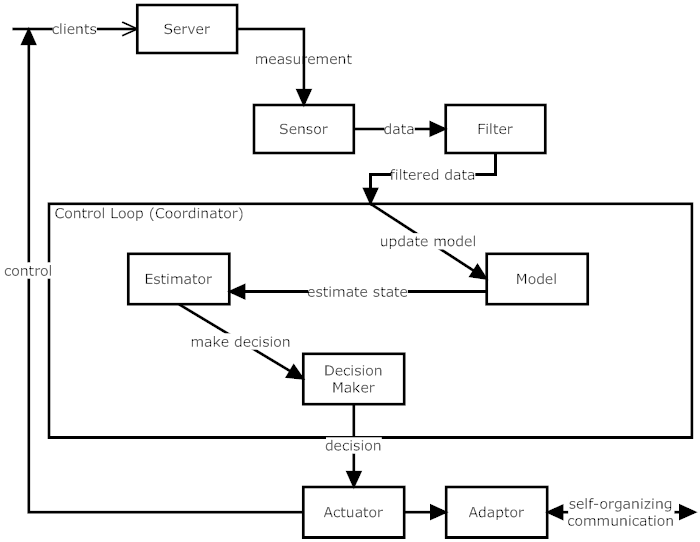
\includegraphics[width=0.9\linewidth]{Self-optimizingControlLoop_full}
	\caption{Self-Optimizing Control Loop Architecture}
	\label{fig:selfopt-archi}
\end{figure}

Each collaborative server can be seen as having one perturbation signal which is the arrival of requests from clients connected to the server. Some requests, like video streaming, are more demanding on the server than others. As requests are processed, the CPU usage and response time of the server will change. More requests or more demanding requests will lead to higher CPU usage and an increase in response time. As the number of requests decreases, the CPU usage and response time will also decrease. Based on the measured sensor data, the control loop uses a fuzzy model and estimator to predict the response time for the next sampling period. This prediction is used in order to decide if the server should accept connections or not. The block diagram can be mapped to the eight component based architecture through the following steps:

\begin{enumerate}
	\item Implement a sensor which measures the desired data from the media server. The measured data includes:
	\begin{enumerate}
		\item CPU usage
		\item Number of connected clients
		\item Number of collaborative rooms
		\item Number of clients connected to all media servers in the cloud
		\item Network latency
		\item Bandwidth up/down
		\item Number of streams incoming/outgoing from server
	\end{enumerate}
	\item Add a filter which computes the numbers of packets in and out from the bandwidth up/down
	\item Add a fuzzy model which calculates the confidence that the server is overloaded. The fuzzy model computes two fuzzy functions:
	\begin{enumerate}
		\item Compute confidence1 based on number of clients, packets out, packets in and number of incoming streams.
		\item Compute confidence2 based on packets in and CPU usage
		\item Take the maximum value of the two confidences
	\end{enumerate}
	\item Add an estimator which compares the confidence from the model with two given thresholds. If the confidence is above the higher threshold increment a counter of how many times the system was above the higher threshold. Similarly if the confidence is bellow the threshold increment a counter of how many time the system was bellow the lower threshold.
	\item Add a decision maker which uses the count of how many times the system was above/bellow the thresholds in the estimator to decide if the server should accept or reject connections. If the server is above the higher threshold for more than a given count, then the server stops accepting new clients. If the server is bellow the lower threshold for a given amount of time and is not accepting clients, then it starts accepting clients.
	\item Add an actuator which communicates with the cloud load balancer. If the server should not accept connections then the actuator sends a message to the load balancer that it should stop redirecting new clients to it. Conversely, if the server should start accepting clients again, then it sends a message that the load balancer can start redirecting clients to it.
	\item The coordinator simply coordinates the control loop and passes messages between model, controller, decision maker and actuator.
\end{enumerate}

The control system for each media server is an application separated from the media server and deployed in a separate container from the media server. It can connect to the media server to retrieve sensor data but has no other interactions with the media server. The control system can also act on behalf of the media server to ask the load balancer to redirect or stop redirecting new clients to the media server. The overall control architecture looks as Figure \ref{fig:control-containers}

\begin{figure}
	\centering
	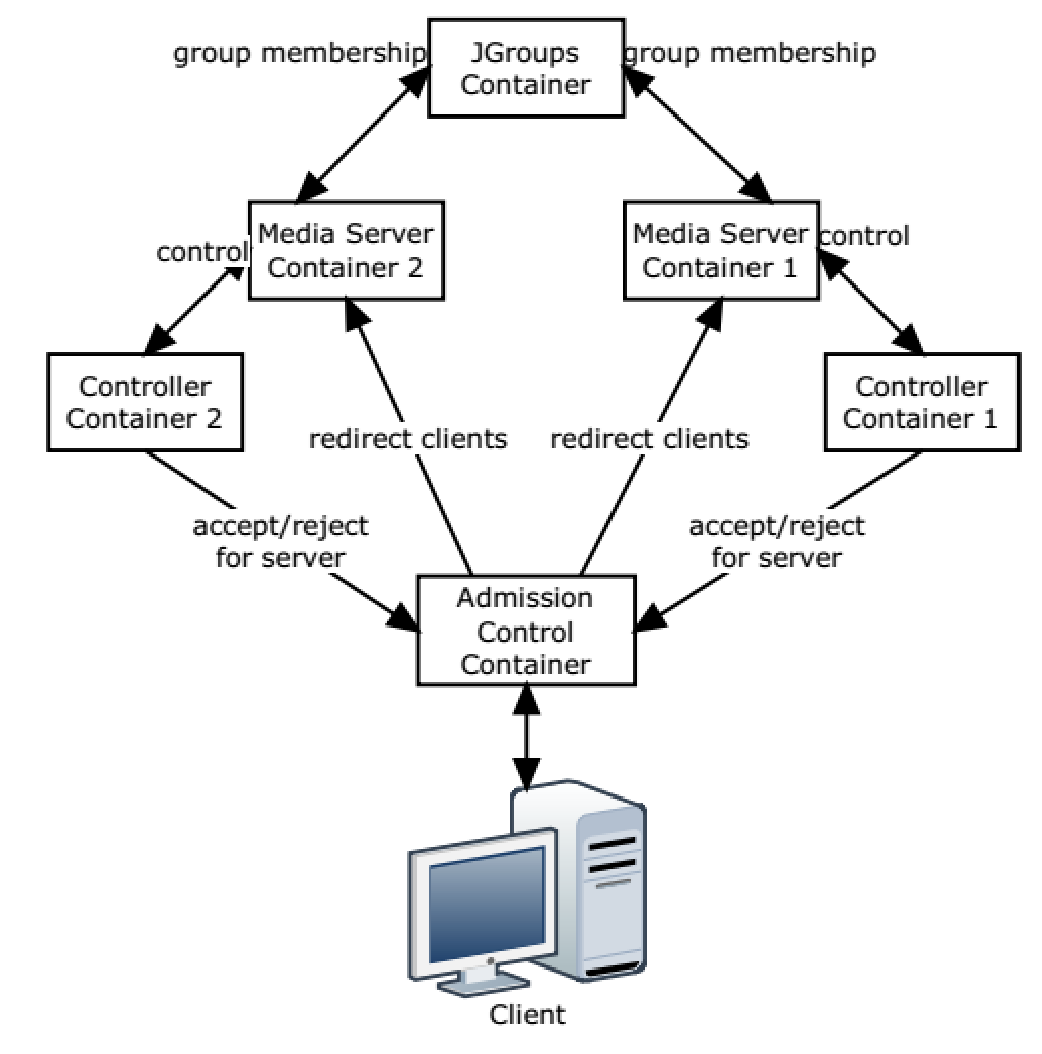
\includegraphics[width=0.9\linewidth]{containers_control}
	\caption{Control System}
	\label{fig:control-containers}
\end{figure}

The results of the fuzzy control system are also fed as an input to the ACO algorithm in order to predict when an SLA breach will happen and serves need to be added or removed from the cloud.

\section{Simulation environment}

The second set of performance tests for the self-organizing management of cloud resources presented in this thesis was a simulation developed on top of the CloudSim and CloudSimEx systems. CloudSim is a framework for modelling and simulating cloud systems in which various tests can be run - for example the placement of tasks in a cloud or the performance of a cloud system. CloudSim allows users to define datacenters which are composed of hosts which can run virtual machines and virtual machines which run on top of the hosts. Both hosts and virtual machines are defined in terms of million instructions per second (MIPS) and memory available. Once a datacenter is defined, a workload can be defined as well to be executed in the datacenter. CloudSim workloads are called cloudlets - a cloudlet represents a user task and defines how many million instructions (MI) the task takes as well as how much memory the task needs. As such a cloudlet's execution time will depend on its' lifetime in MIs and how many MIPS the VM the cloudlet is allocated to has. The usage of MIPS and MI to represent loads and available resources make it complicated to define workloads that would represent real world behaviours.

CloudSimEx extends CloudSim by adding the concept of web sessions. Internally a web session is composed of a number of web cloudlets, where each web cloudlet has a small RAM and MIPS requirements and later web cloudlets in a web session can not be completed until all previous web cloudlets have completed. Web sessions also have the property of targeting both application server VMs and database VMs, with the web session alternating cloudlets running on either application server or database server. Furthermore, CloudSimEx also adds the concept of scaling policies which can be applied on a cloud. A scaling policy adds or removes servers to/from the cloud when the policy determines that some conditions are breached. A basic policy is implemented in CloudSimEx which scales the cloud when the CPU usage passes certain thresholds and also includes a quiet time after a scaling action has been performed. The basic policy implements an interface which makes it easy to add other scaling policies. 

Because CloudSim and CloudSimEx only include CPU usage and memory usage as measurable metrics, the simulation of the self-organizing system uses the CPU usage as an input for the ACO algorithm to determine how the pheromone should be updated. In order to run the self-organizing system in this thesis and compare it to existing results, a number of workloads which are predefined in CloudSimEx are used.

The architecture of the simulation framework is presented in Figure \ref{fig:simulation-design}.


\begin{figure}
	\centering
	\includegraphics[width=0.9\linewidth]{simulation_design}
	\caption{Simulation Framework System}
	\label{fig:simulation-design}
\end{figure}

%description of 

 % Example Implementation

\chapter{Performance results for self-optimizing cloud} % Write in your own chapter title
\label{Chapter_performance}
\lhead{Chapter \ref{Chapter_performance}. \emph{Performance results for self-optimizing cloud}} % Write in your own chapter title to set the page header

\section{Test-bed Autonomic Computing Performance Tests}

This section will present the performance of the self-organizing, self-optimizing autonomic system presented in this thesis when run on top of the test bed under various loads. The goal of this section is to determine how the system behaves when being overloaded or underloaded.

The tests are split such that the same scenario is tested with various numbers of starting servers in the cluster and various loads such that up scaling, down scaling and no scaling are all tested. The tests are run slightly longer than 30 minutes, due to the fact that there is a ramp up at the beginning of the test while clients join, sessions are created and clients start streaming.

\subsection{Single server start}

The first set of tests starts with a single server in the cloud. In this case, if the cloud is underloaded the server will not be removed from the cloud as that will leave no servers servicing user requests.

\subsubsection{Under-load cloud}

This test case tests the base case of an under-loaded cloud, where the cloud contains a single server and the number of clients and streams can be easily handled by the single server.

Figure \ref{fig:1serv-ant} shows the pheromone level as seen by the ant. The top and bottom dotted red lines represent the thresholds for adding/removing servers to/from the cloud. The middle dotted blue line represents the starting pheromone level. When the pheromone passes the higher threshold servers are removed and when the pheromone passes the lower threshold servers are added to the cloud. Once the threshold is passed the ant goes to the manager which attempts to optimize the cloud's server count - this can be observed at the top of the graph where it plateaus as that is time when the ant is at the manager. In this case the optimization will result in no change as this is the only server in the cloud and it can not be removed. After optimization the ant returns to the server and restarts the process from the base state of the system. Figure \ref{fig:1serv-pher} shows the pheromone as seen at the server. Since there is one server and one ant the values are very close, however in the server figure the pheromone decay can also be observed. 

Finally, figure \ref{fig:1serv-perf} shows the performance of the server. The optimization of the system starts at the same time the first stream begins seen on the bandwidth graph when the bandwidth value goes up. In this case it can be seen that the CPU is barely used and also latencies are low and bandwidth is not high, as such the system wishes to remove servers from the cloud.

\begin{figure}
	\centering
		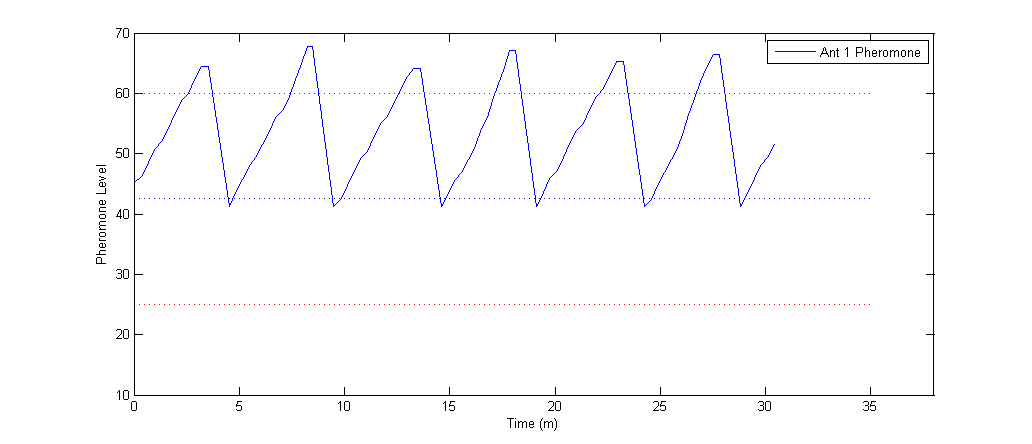
\includegraphics[width=0.95\columnwidth]{results/Run-1-low/ant-1.png}
	\caption{Under-loaded cloud - Pheromone as seen by Ant 1}
	\label{fig:1serv-ant}
\end{figure}

\begin{figure}
	\centering
		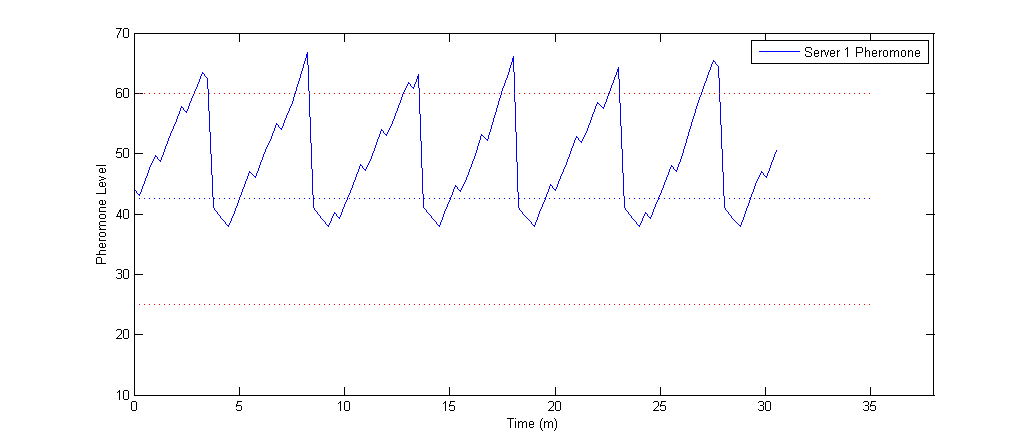
\includegraphics[width=0.95\columnwidth]{results/Run-1-low/server-1.png}
	\caption{Under-loaded cloud - Pheromone as seen by Server 1}
	\label{fig:1serv-pher}
\end{figure}

\begin{figure}
	\centering
		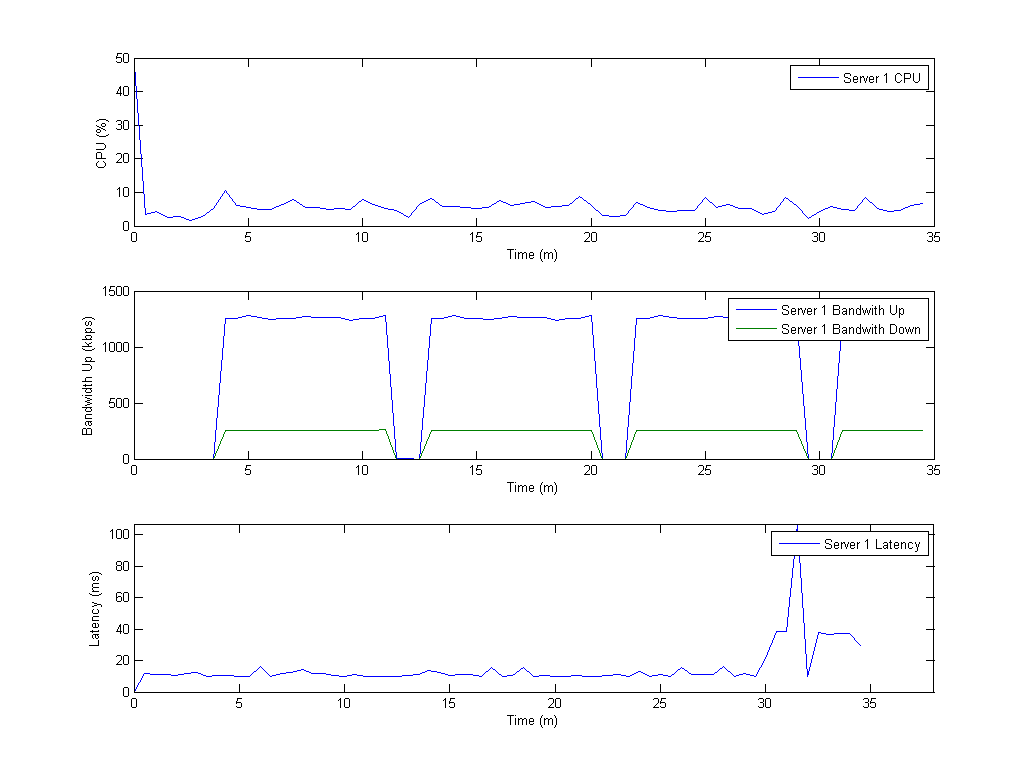
\includegraphics[width=0.95\columnwidth]{results/Run-1-low/perf-1.png}
	\caption{Under-loaded cloud - Server 1 performance}
	\label{fig:1serv-perf}
\end{figure}

\subsubsection{Medium/low loaded cloud}

In this test case the cloud is still underloaded but the load is closer to what a single server can support. As such it can be seen that in figure \ref{fig:1serv-ant-lowmed} the pheromone level increases slower than in figure \ref{fig:1serv-ant} and similarly for figures \ref{fig:1serv-pher-lowmed} and figure \ref{fig:1serv-pher-lowmed}. At the same time figure  \ref{fig:1serv-perf-lowmed} shows that the CPU usage is higher than in the previous test case, while bandwidth usage and latencies are also higher.

\begin{figure}[!ht]
	\centering
		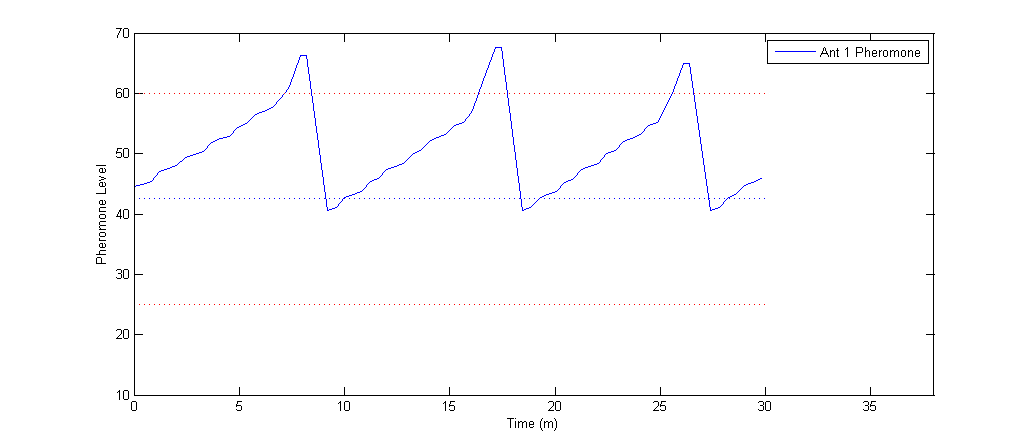
\includegraphics[width=0.95\columnwidth]{results/Run-1-lowmed/ant-1.png}
	\caption{Medium/low loaded cloud - Pheromone as seen by Ant 1}
	\label{fig:1serv-ant-lowmed}
\end{figure}

\begin{figure}
	\centering
		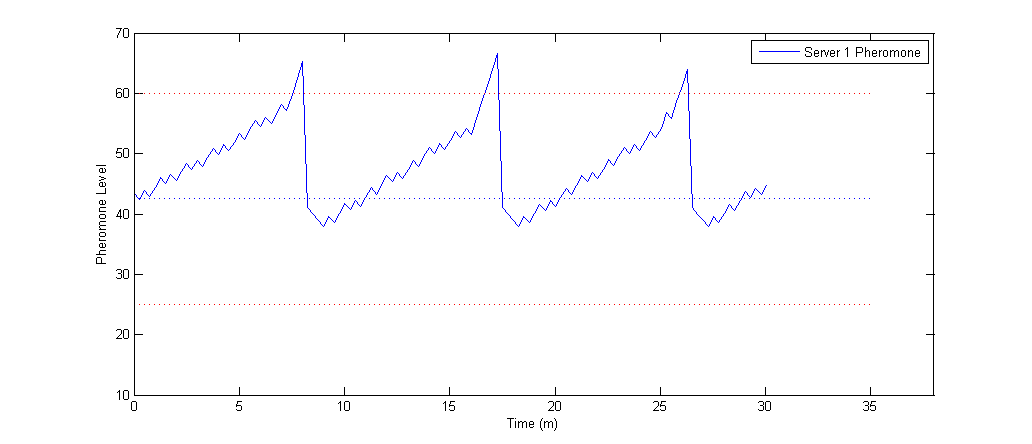
\includegraphics[width=0.95\columnwidth]{results/Run-1-lowmed/server-1.png}
	\caption{Medium/low loaded cloud - Pheromone as seen by Server 1}
	\label{fig:1serv-pher-lowmed}
\end{figure}

\begin{figure}
	\centering
		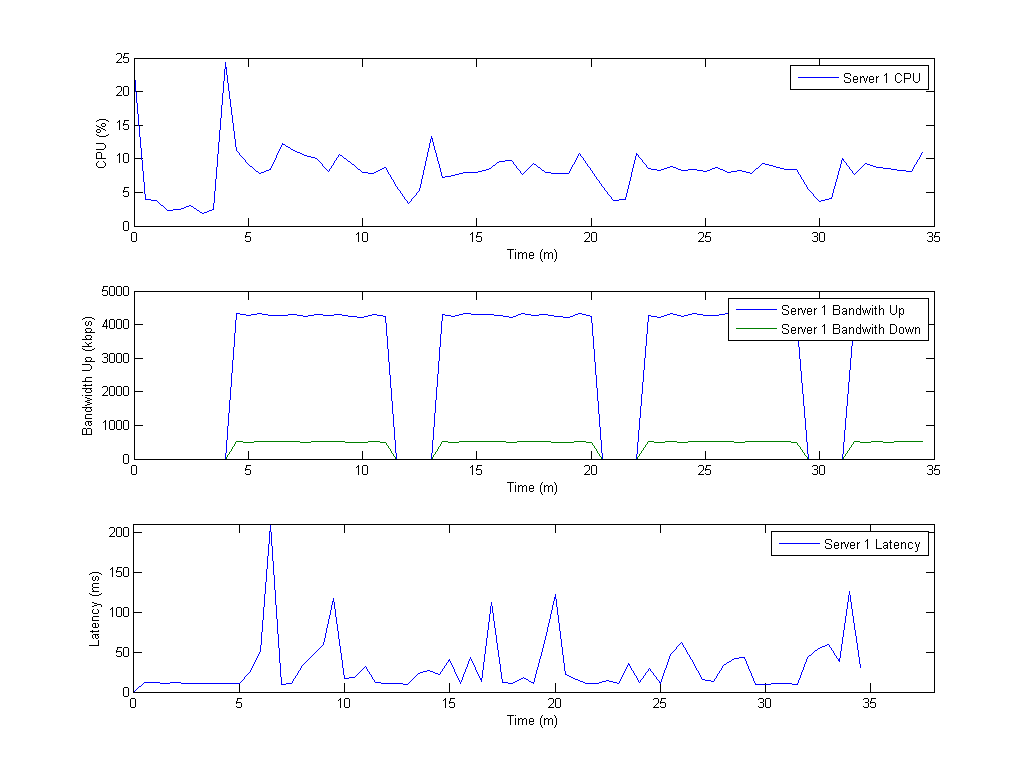
\includegraphics[width=0.95\columnwidth]{results/Run-1-lowmed/perf-1.png}
	\caption{Medium/low loaded cloud - Server 1 performance}
	\label{fig:1serv-perf-lowmed}
\end{figure}

\subsubsection{Medium loaded cloud}

This test case tests a server which is neither overloaded nor underloaded. As such, the pheromone level should stay stable such that servers are not added or removed from the cloud. As seen in graphs \ref{fig:1serv-ant-med} and \ref{fig:1serv-pher-med} the pheromone level is largely stable except for two spikes around 14 and 29 minutes in. The two spikes coincide with the streams stopping and in figure \ref{fig:1serv-perf-med} it can be noticed that at those times the CPU usage and latency drops down, resulting in the server being underloaded for a brief period of time.

\begin{figure}[!ht]
	\centering
		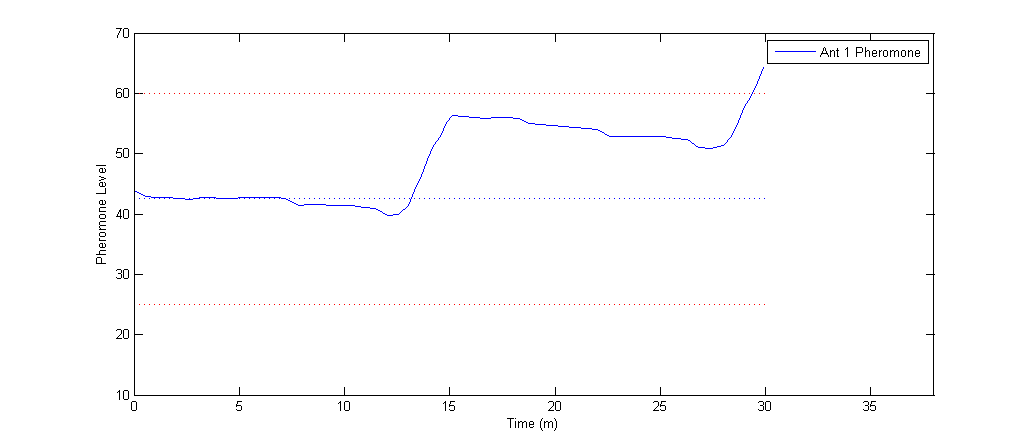
\includegraphics[width=0.95\columnwidth]{results/Run-1-med/ant-1.png}
	\caption{Medium loaded cloud - Pheromone as seen by Ant 1}
	\label{fig:1serv-ant-med}
\end{figure}

\begin{figure}
	\centering
		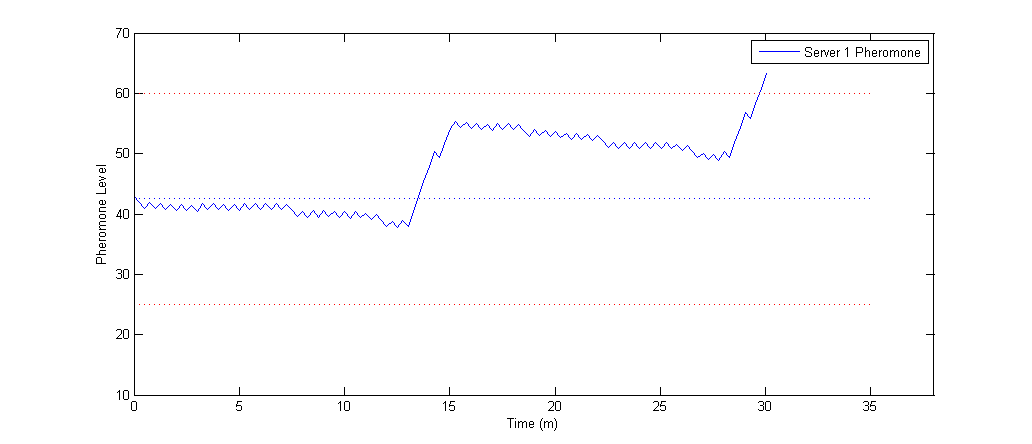
\includegraphics[width=0.95\columnwidth]{results/Run-1-med/server-1.png}
	\caption{Medium loaded cloud - Pheromone as seen by Server 1}
	\label{fig:1serv-pher-med}
\end{figure}

\begin{figure}
	\centering
		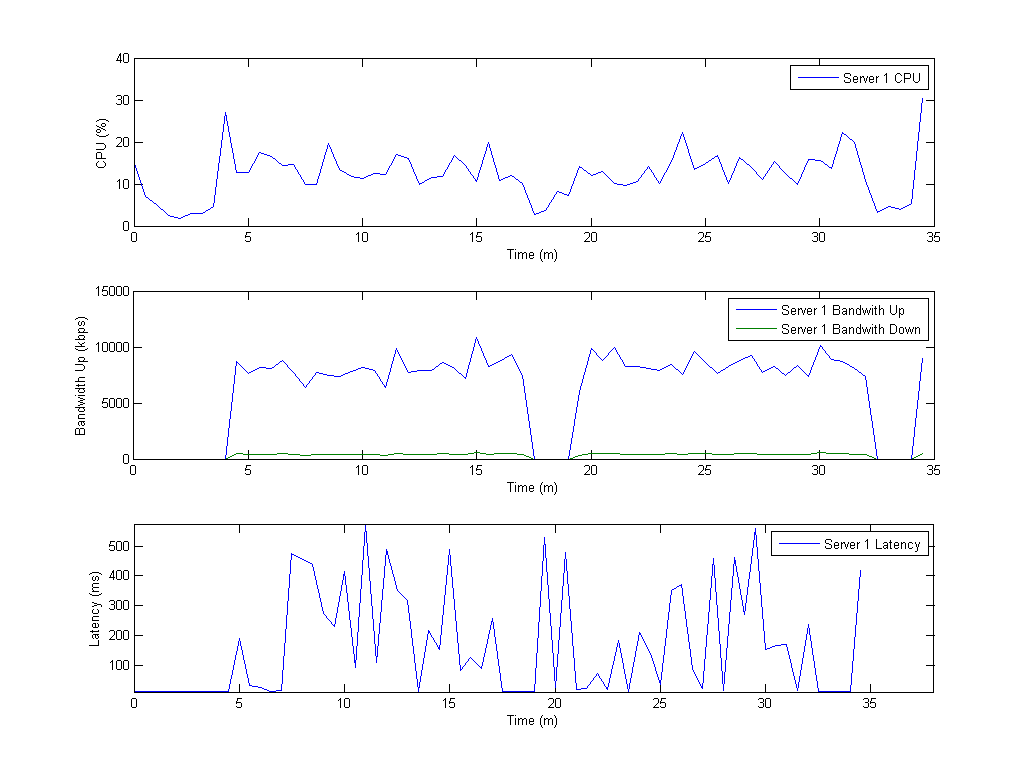
\includegraphics[width=0.95\columnwidth]{results/Run-1-med/perf-1.png}
	\caption{Medium loaded cloud - Server 1 performance}
	\label{fig:1serv-perf-med}
\end{figure}

\subsubsection{Medium/high loaded cloud}

In this test case the cloud is overloaded but barely above what a single server can accommodate. Looking at graph \ref{fig:1serv-pher-medhigh} it can be noticed that the pheromone level drops for the first 12 - 13 minutes after which a second server is added, which can be noticed by the second server appearing on the graph.  Because two servers are two much for this load the pheromone level increases until the thresholds are breached again and one of the servers is stopped. Figure \ref{fig:1serv-pher-medhigh} shows the pheromone at the two servers and matches what the ants see as well.

The performance graphs show high bandwidth and high CPU usage until the second server is added, at which time the cloud is rebalanced and the bandwdith and CPU are lower for each of the two servers. Average latency for the clients also drops when the second server is added.

\begin{figure}
	\centering
		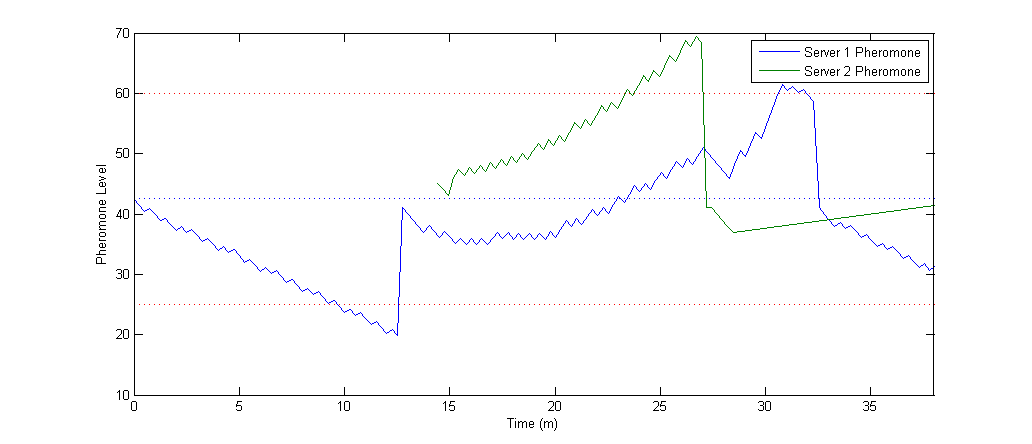
\includegraphics[width=0.95\columnwidth]{results/Run-1-medhigh/server-1.png}
	\caption{Medium/high loaded cloud - Pheromone as seen by servers}
	\label{fig:1serv-pher-medhigh}
\end{figure}

\begin{figure}
	\centering
		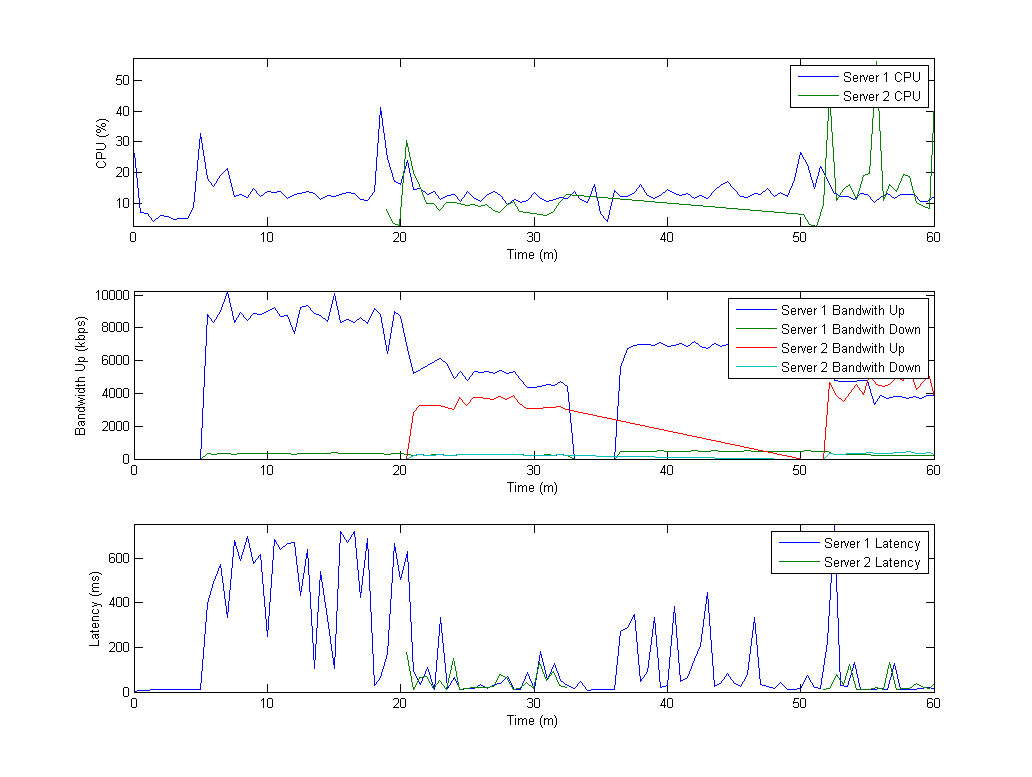
\includegraphics[width=0.95\columnwidth]{results/Run-1-medhigh/perf-1.png}
	\caption{Medium/high loaded cloud - Server performance}
	\label{fig:1serv-perf-medhigh}
\end{figure}

In terms of optimization by the house hunting algorithm the up scaling of the cloud is trivial as there is a single ant so there is no recruitment needed. When the cloud is down scaled however the house hunting algorithm runs. In the first round each of the two ants chooses a new server count - in this case both choose to remove one server and then they simulate the solution. One ant's solution fitness is 0.519 while the other ant's is 0.497. The ants then go through recruitment and the ant with fitness 0.497 recruits the other ant to it's nest. Because all ants at this point go to the same nest, this is the solution of the optimization and one of the servers is removed.

\subsubsection{Over-loaded cloud}

This test is set up such that a single server can not handle by itself the requests sent by clients, and as such it is expected that a second server will be added to the cloud and not be removed. This can be seen in figure \ref{fig:1serv-pher-high} as the pheromone level drops initially very fast until a second server is added. After the second server is added the pheromone level increases for some time but stabilizes after that. While server two has a pheromone level higher than the upper threshold, the average pheromone across the cloud is bellow the thresholds. 

The performance graphs show high CPU, bandwidth and latency before the second server is added. After the second server is added the performance metrics stabilize at good values. The optimization by the house hunting algorithm is also trivial as there is a single ant to begin with, so no recruitment can happen.

\begin{figure}
	\centering
		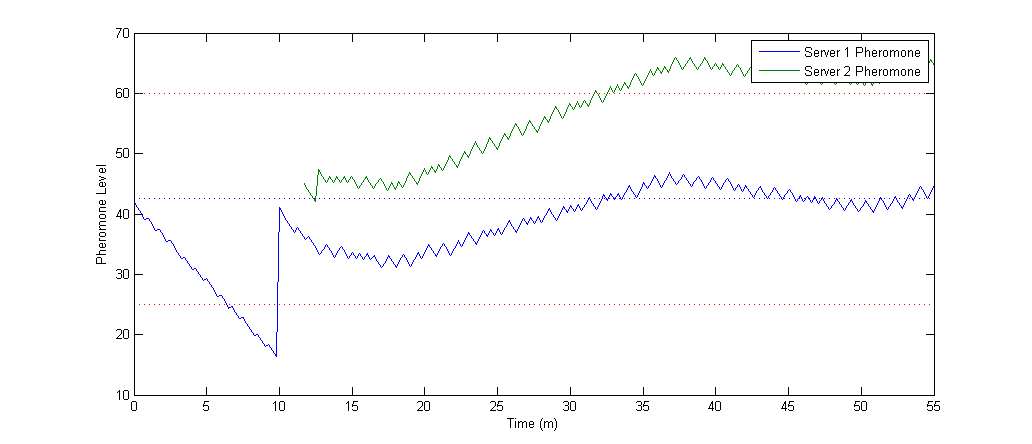
\includegraphics[width=0.95\columnwidth]{results/Run-1-high/server-1.png}
	\caption{Over-loaded cloud - Pheromone as seen by servers}
	\label{fig:1serv-pher-high}
\end{figure}

\begin{figure}
	\centering
		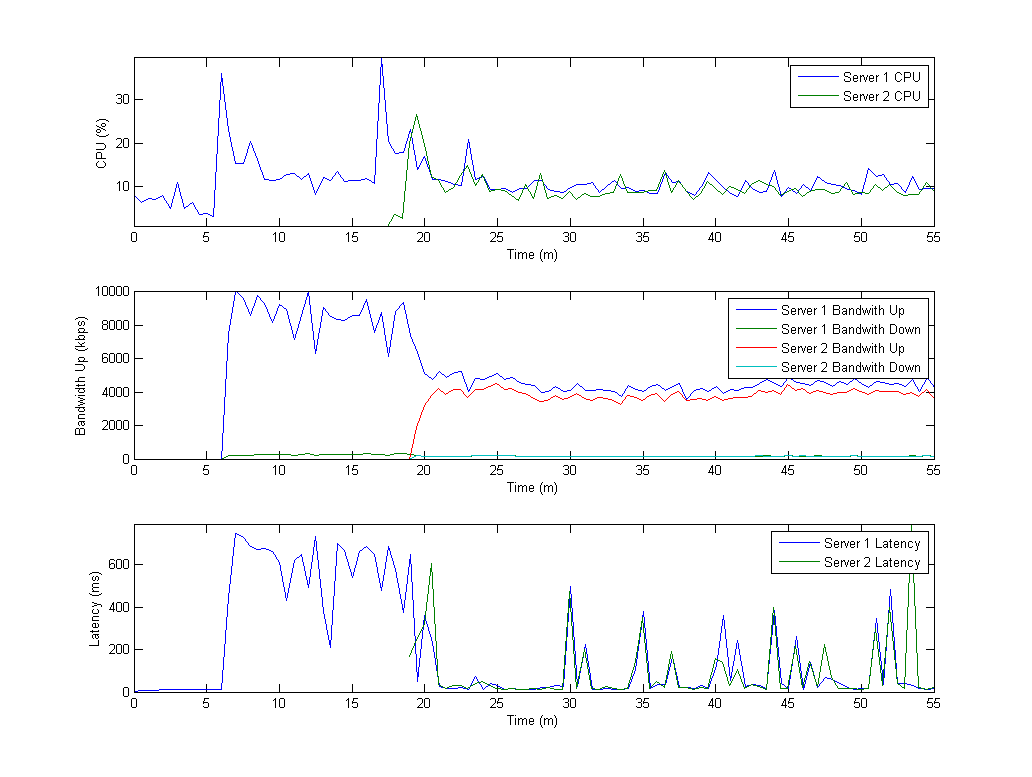
\includegraphics[width=0.95\columnwidth]{results/Run-1-high/perf-1.png}
	\caption{Over-loaded cloud - Server performance}
	\label{fig:1serv-perf-high}
\end{figure}

\subsection{Two server start}

This set of tests start with two servers in the cloud and different loads.

\subsubsection{Under-load cloud}

This test case tests the base case of an under-loaded cloud, where the cloud starts with two servers but the number of clients and streams can be easily handled by a single server. Figure \ref{fig:2serv-pher-low} shows the pheromone level from the server's perspective. The pheromone goes up at both servers and after the threshold is reached one of the two servers is removed. After the removal the load is still too low for the single server and the pheromone level continues increasing. 

The server performance graphs show that the servers are under-loaded and even after the server is removed the load on the single remaining server is low enough not to cause a breach of SLA.

\begin{figure}
	\centering
		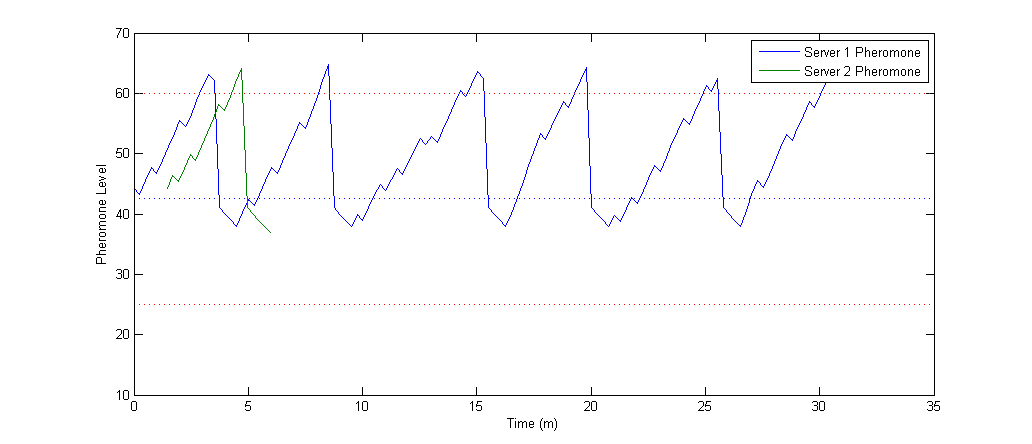
\includegraphics[width=0.75\columnwidth]{results/Run-2-low/server-1.png}
	\caption{Under-loaded cloud - Pheromone as seen by servers}
	\label{fig:2serv-pher-low}
\end{figure}

\begin{figure}
	\centering
		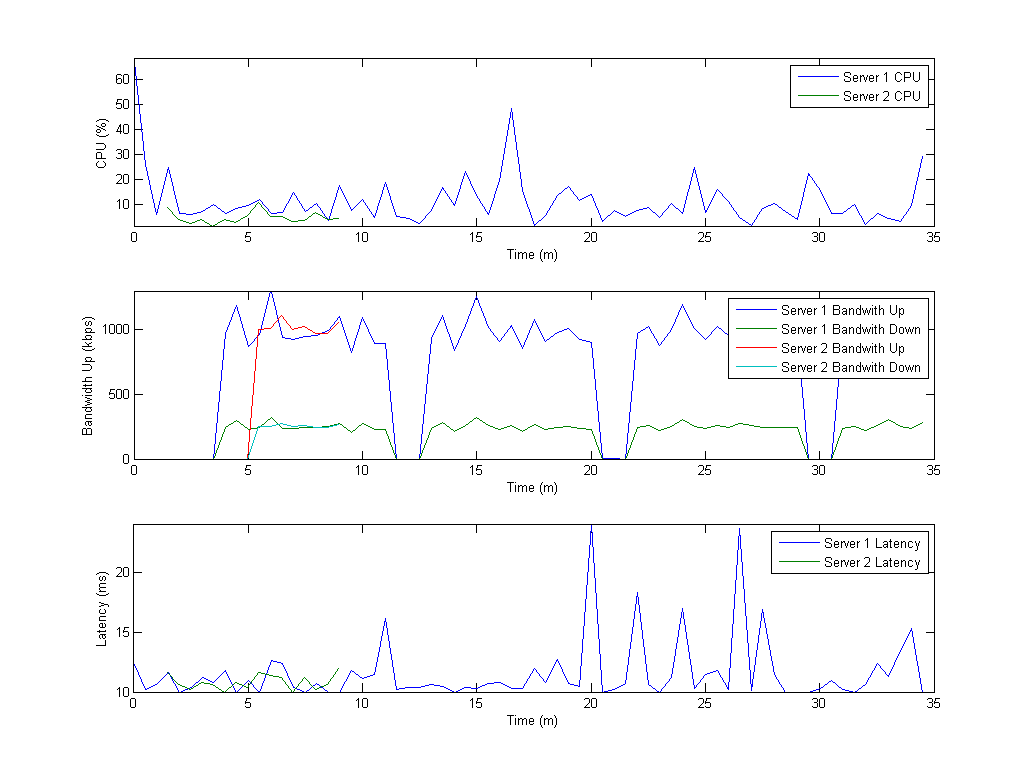
\includegraphics[width=0.75\columnwidth]{results/Run-2-low/perf-1.png}
	\caption{Under-loaded cloud - Server performance}
	\label{fig:2serv-perf-low}
\end{figure}

\subsubsection{Medium/low loaded cloud}

Similarly to the previous test, this test does not generate enough load for both servers. Unlike the previous test, which has a very low load, the load in this test is closer to the load of a well balanced cloud. Figure \ref{fig:2serv-pher-medlow} shows the pheromone as seen by the server. The pheromone increases similar to the previous test but at a lower rate. As before, the load is quite low on the two servers and once one of the two servers is removed the other server can take the load without problems.

\begin{figure}
	\centering
		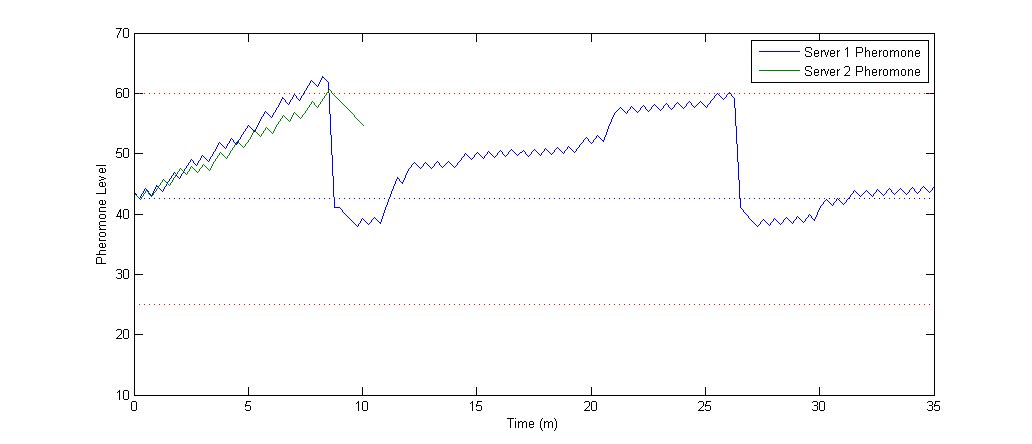
\includegraphics[width=0.75\columnwidth]{results/Run-2-lowmed/server-1.png}
	\caption{Medium/low loaded cloud - Pheromone as seen by servers}
	\label{fig:2serv-pher-medlow}
\end{figure}

\begin{figure}
	\centering
		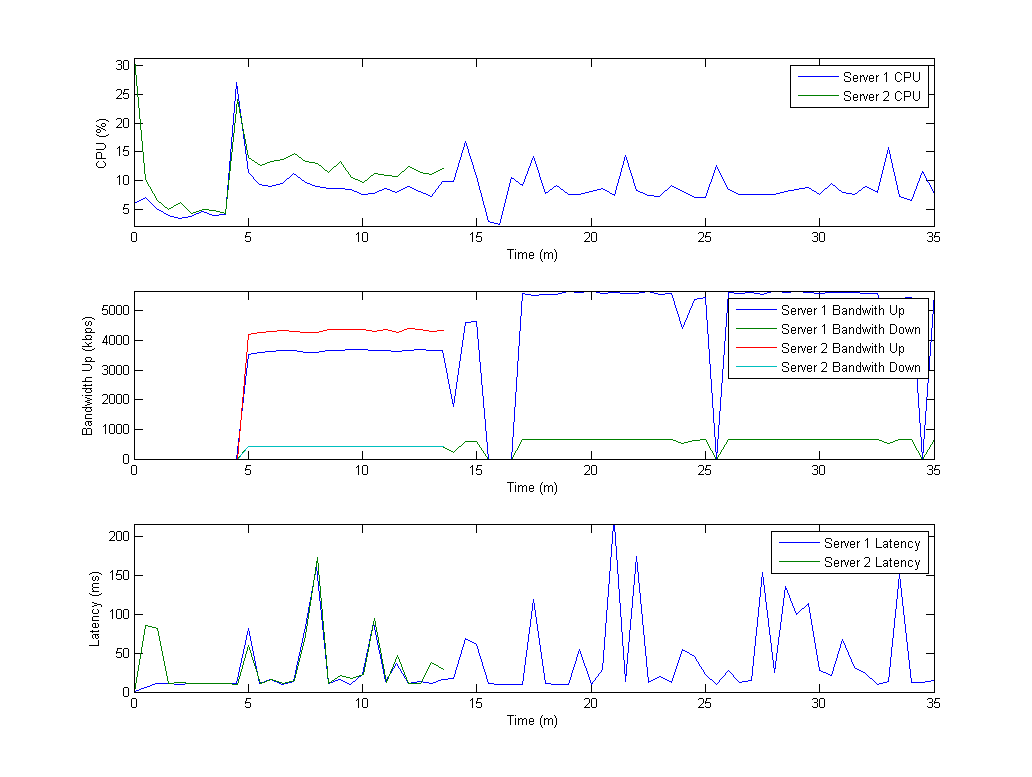
\includegraphics[width=0.75\columnwidth]{results/Run-2-lowmed/perf-1.png}
	\caption{Medium/low loaded cloud - Server performance}
	\label{fig:2serv-perf-medlow}
\end{figure}

\subsubsection{Medium loaded cloud}

This test case puts enough load on the cloud to require two servers to provide good QoS to the clients. Figure \ref{fig:2serv-pher-med} shows the pheromone levels as seen at the servers. Looking at the performance graphs in figure \ref{fig:2serv-perf-med} it can be noticed that the two servers are not perfectly balanced as server 2 has a lower load than server 1 as seen by CPU utilization, bandwidth and latency. As such, the pheromone level at server 2 increases while the pheromone level at server 1 stays stable. Even though one server has increasing pheromone values no servers are removed because the ants history has a lower average pheromone than the threshold.

\begin{figure}
	\centering
		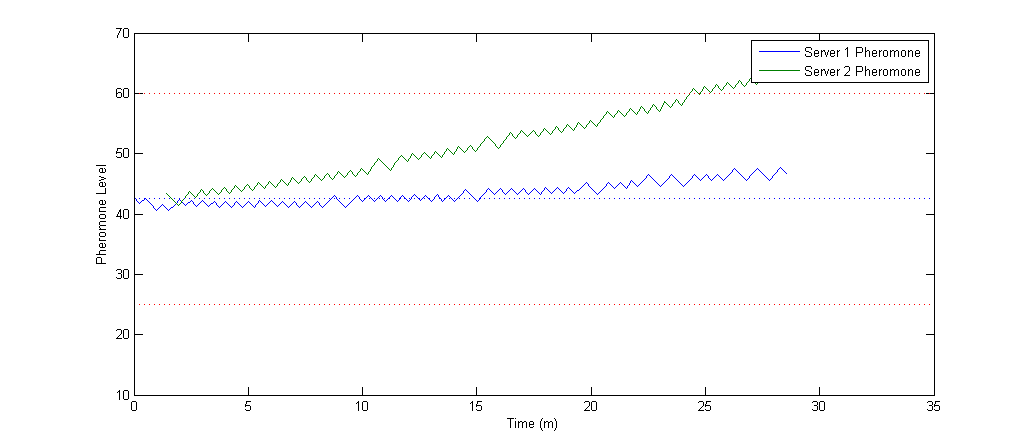
\includegraphics[width=0.75\columnwidth]{results/Run-2-med/server-1.png}
	\caption{Medium loaded cloud - Pheromone as seen by servers}
	\label{fig:2serv-pher-med}
\end{figure}

\begin{figure}
	\centering
		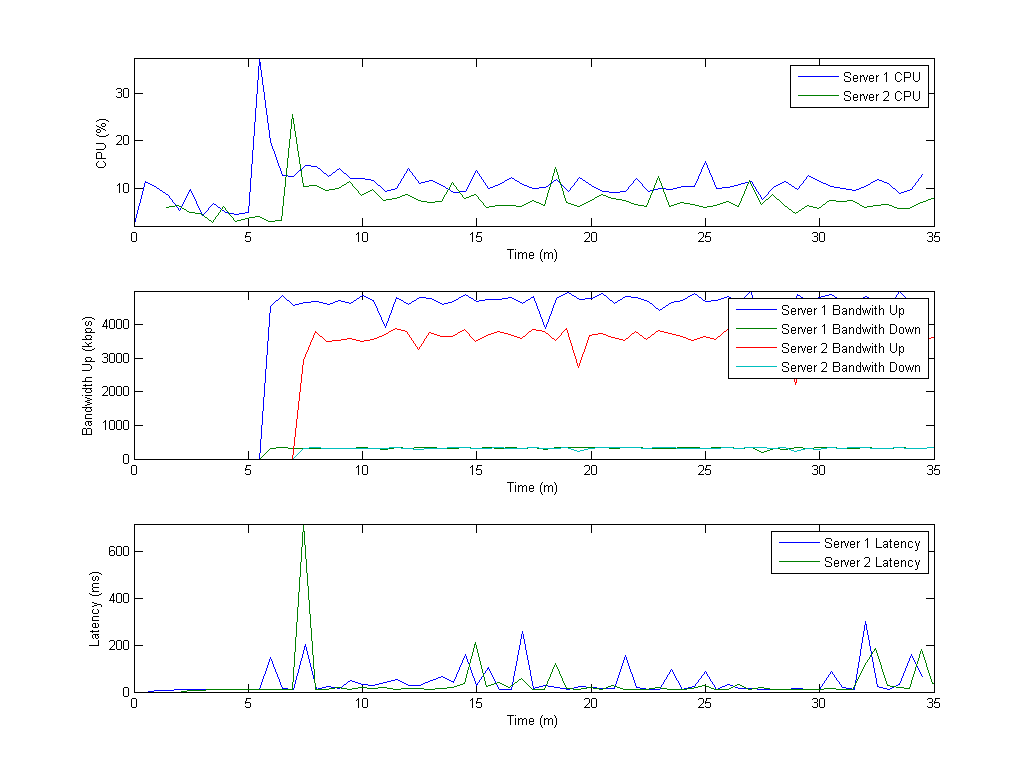
\includegraphics[width=0.75\columnwidth]{results/Run-2-med/perf-1.png}
	\caption{Medium loaded cloud - Server performance}
	\label{fig:2serv-perf-med}
\end{figure}

\subsubsection{Medium/high loaded cloud}

In this test the load is higher than what two servers can support but not by a significant amount. Initially in figure \ref{fig:2serv-pher-medhigh} the pheromone level drops at the beginning of the test. After the threshold is breached one new server is added. After the server is added the system is largely stable, however due to the servers not being balanced server 1 sees an increase in pheromone levels. This increase however is not enough to cause a SLA breach as the other two servers are within proper bounds.

Performance graphs show that the two servers are overloaded in the beginning and after the addition of the new servers, the system becomes stable until the end of the test.

\begin{figure}
	\centering
		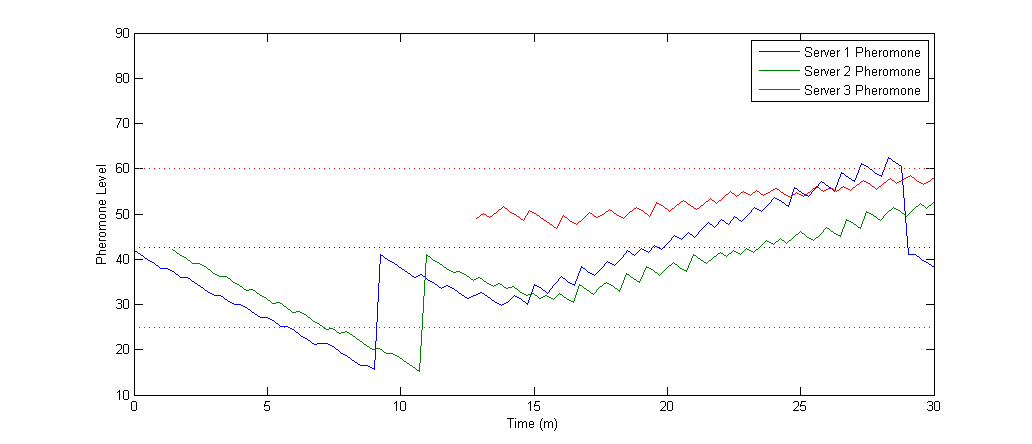
\includegraphics[width=0.75\columnwidth]{results/Run-2-medhigh/server-1.png}
	\caption{Medium/high loaded cloud - Pheromone as seen by servers}
	\label{fig:2serv-pher-medhigh}
\end{figure}

\begin{figure}
	\centering
		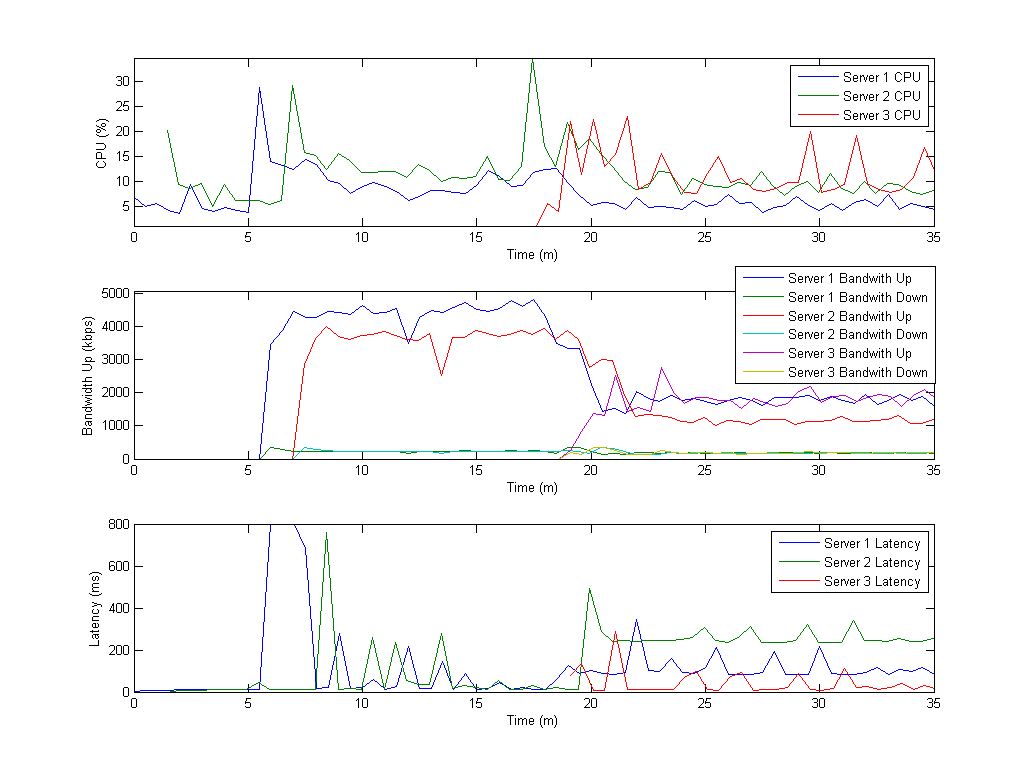
\includegraphics[width=0.75\columnwidth]{results/Run-2-medhigh/perf-1.png}
	\caption{Medium/high loaded cloud - Server performance}
	\label{fig:2serv-perf-medhigh}
\end{figure}

\subsubsection{Over loaded cloud}

Finally a test was run where the cloud is overloaded significantly for two servers. This can be seen in figure \ref{fig:2serv-pher-high} as the pheromone level drops at the beginning of the test. After the threshold is breached two new servers are added. Because after the two servers are added the cloud is not well balanced server 1 sees an increase in pheromone, while servers 3 and 4 see a decrease with server 2 being stable. Once server 1 stabilizes however, there are too many servers in the cloud due to the fact that the clients stop streaming. As such the servers are removed until one server remains in the cloud.

Performance graphs show that the two servers are overloaded in the beginning and after the addition of the two new servers, the system becomes stable until the end of the test.

\begin{figure}
	\centering
		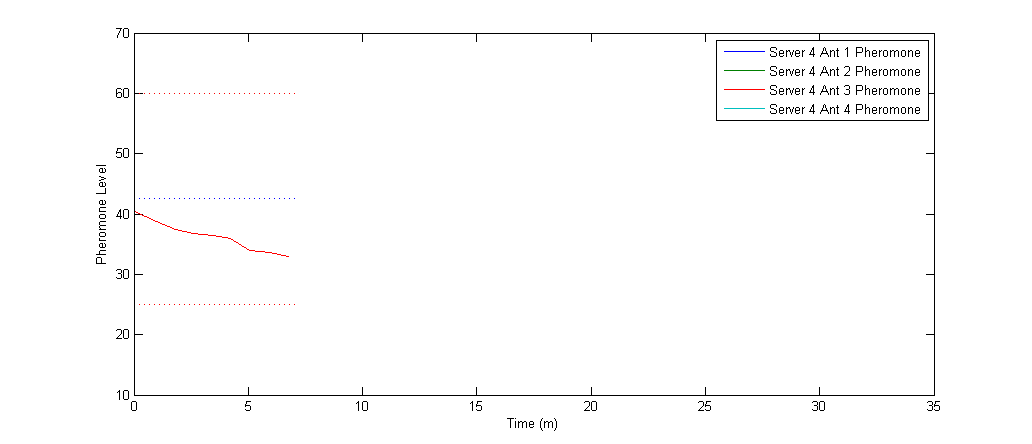
\includegraphics[width=0.75\columnwidth]{results/Run-2-high/ant-13.png}
	\caption{Over-loaded cloud - Pheromone at Server 4 as seen by ants}
	\label{fig:2serv-ant13-high}
\end{figure}

\begin{figure}
	\centering
		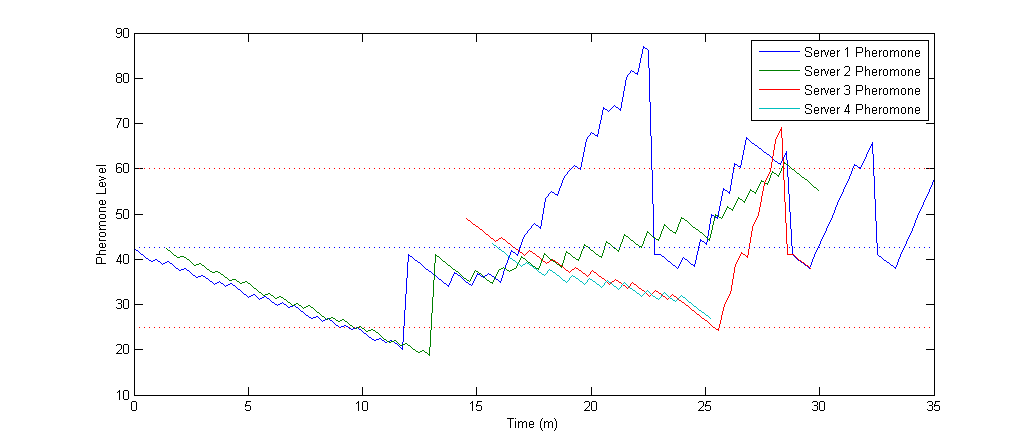
\includegraphics[width=0.75\columnwidth]{results/Run-2-high/server-1.png}
	\caption{Over-loaded cloud - Pheromone as seen by servers}
	\label{fig:2serv-pher-high}
\end{figure}

\begin{figure}
	\centering
		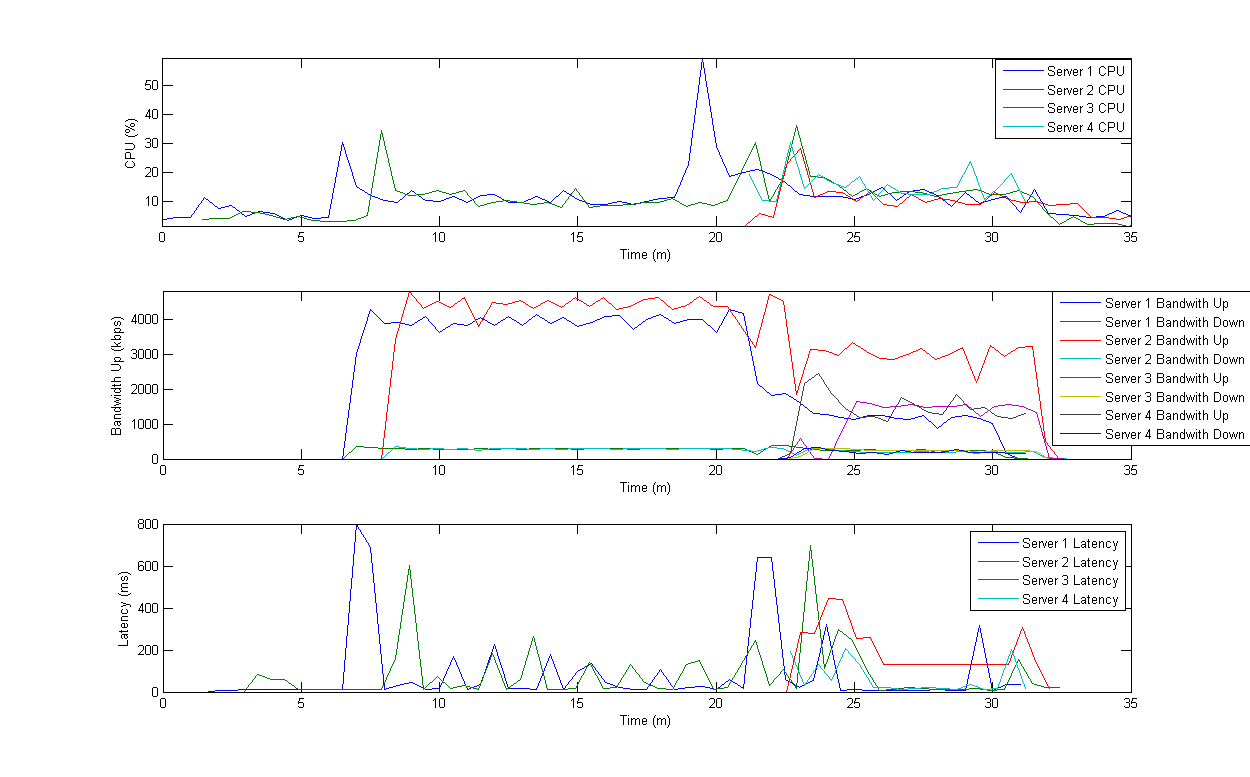
\includegraphics[width=0.75\columnwidth]{results/Run-2-high/perf-1.png}
	\caption{Over-loaded cloud - Server performance}
	\label{fig:2serv-perf-high}
\end{figure}

\subsection{Three server start}

This set of tests start with three servers in the cloud and different loads.

\subsubsection{Under loaded cloud}

Similar to the other cases the first test is started with a load which a single server can easily meet. As seen in figure \ref{fig:3serv-pher-low} the pheromone level increases, and one of the server is removed. After the removal the pheromone level continues to increase but slower since a single server is sufficient. After the threshold is reached again a second server is removed and the cloud stabilizes. The performance graphs show that the load is taken by the other remaining server without any problems.

For the house hunting optimization once the ants simulate the solutions, the initial state is that two of the ants want to remove 2 servers while one of the ants wishes to remove a single server.

\begin{enumerate}
	\item Initial solutions: 
	\begin{itemize}
		\item Ant 1 goes to Nest 1 - remove one servers
		\item Ant 2 goes to Nest 2 - remove two servers
		\item Ant 3 goes to Nest 3 - remove two server
	\end{itemize}
	\item Recruitment:
	\begin{itemize}
		\item Ant 1 recruits Ant 2 and nest 2 is dropped out as no ants go to it
		\item Ant 3 recruits a newly created ant which looks like Ant 3
	\end{itemize}
	\item Recruitment:
	\begin{itemize}
		\item Ant 1 recruits Ant 4
		\item Ant 2 recruits Ant 3
	\end{itemize}
	\item All ants go to same solution which is nest 1
\end{enumerate}

\begin{figure}
	\centering
		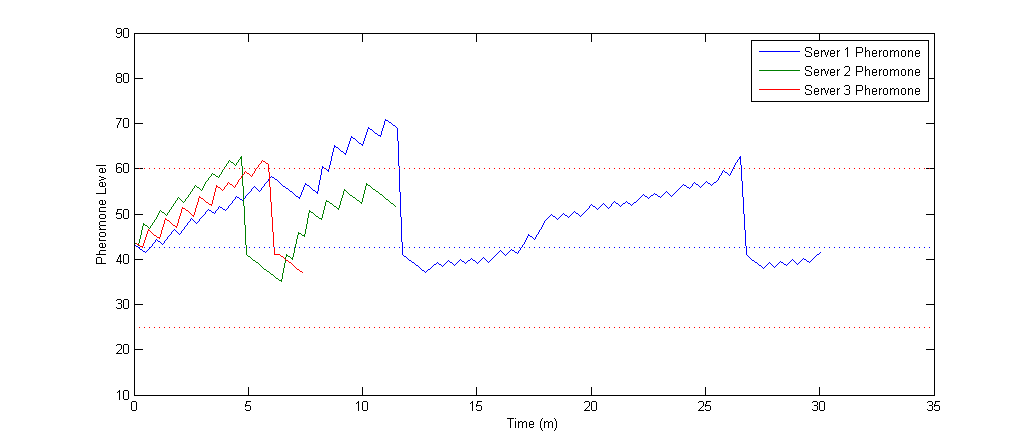
\includegraphics[width=0.75\columnwidth]{results/Run-3-low/server-1.png}
	\caption{Under loaded cloud - Pheromone as seen by servers}
	\label{fig:3serv-pher-low}
\end{figure}

\begin{figure}
	\centering
		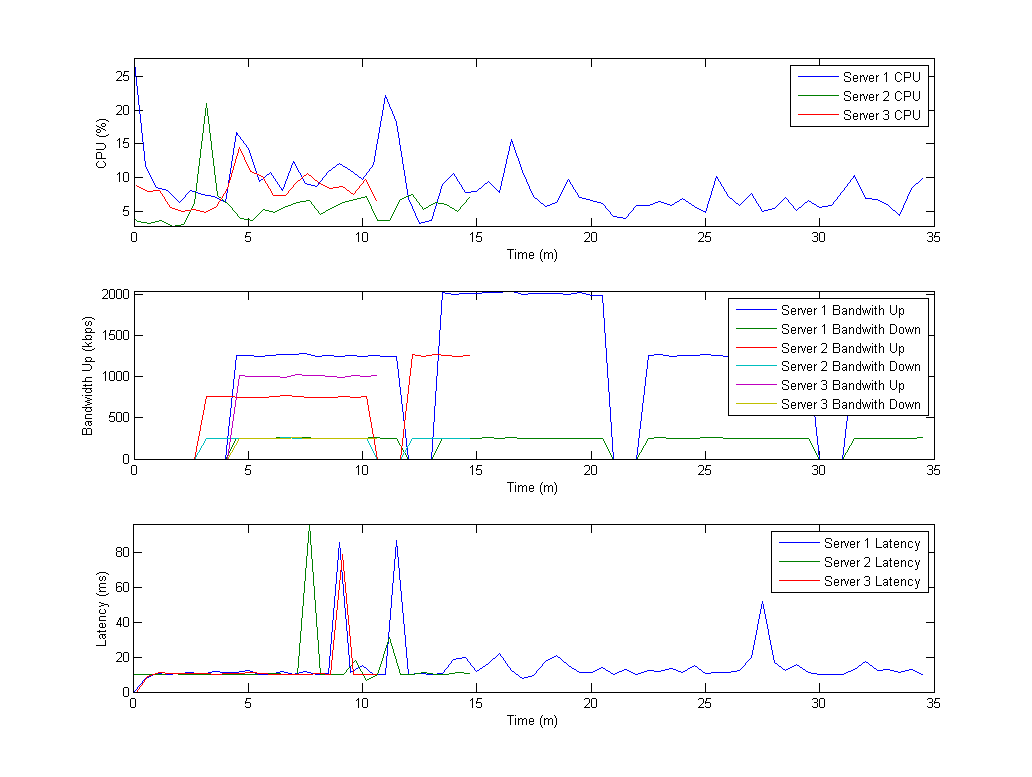
\includegraphics[width=0.75\columnwidth]{results/Run-3-low/perf-1.png}
	\caption{Under loaded cloud - Server performance}
	\label{fig:3serv-perf-low}
\end{figure}

\subsubsection{Medium/low loaded cloud}

In the medium/low scenario the pheromone level increases slower than in the underloaded scenario as one server is sufficient for the workload, but it would put more strain on a single server as seen in figure \ref{fig:3serv-perf-lowmed}. In this case, once the threshold is reached, the house hunting optimization chooses to remove two servers. The initial solution set all choose to remove two servers, however the system still goes through the house hunting optimization algorithm.

\begin{enumerate}
	\item Initial solutions: 
	\begin{itemize}
		\item Ant 1 goes to Nest 1 - remove two servers
		\item Ant 2 goes to Nest 2 - remove two servers
		\item Ant 3 goes to Nest 3 - remove two servers
	\end{itemize}
	\item Recruitment:
	\begin{itemize}
		\item Ant 2 recruits Ant 1 and nest 1 is dropped out as no ants go to it
		\item Ant 3 recruits a newly created ant which looks like Ant 3
	\end{itemize}
	\item Recruitment:
	\begin{itemize}
		\item Ant 2 recruits Ant 3
		\item Ant 1 recruits Ant 4
	\end{itemize}
	\item All ants go to same solution which is nest 2
\end{enumerate}

\begin{figure}
	\centering
		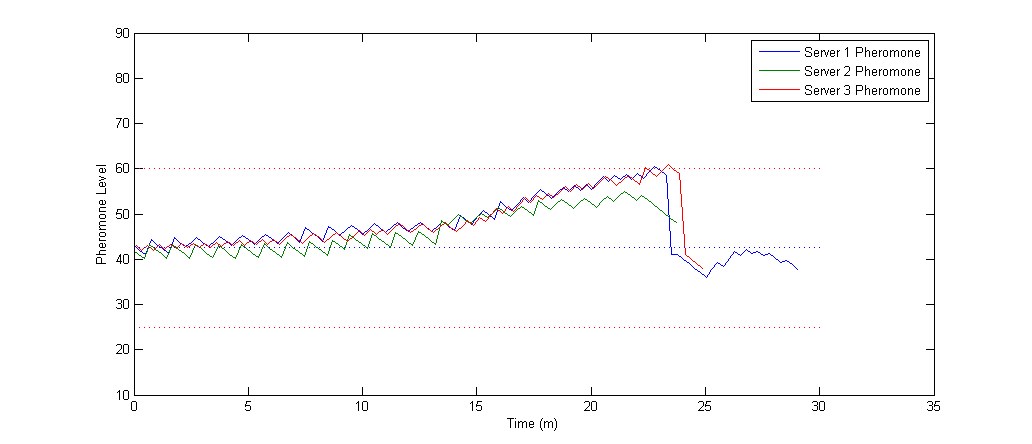
\includegraphics[width=0.75\columnwidth]{results/Run-3-lowmed/server-1.png}
	\caption{Medium/low loaded cloud - Pheromone as seen by servers}
	\label{fig:3serv-pher-lowmed}
\end{figure}

\begin{figure}
	\centering
		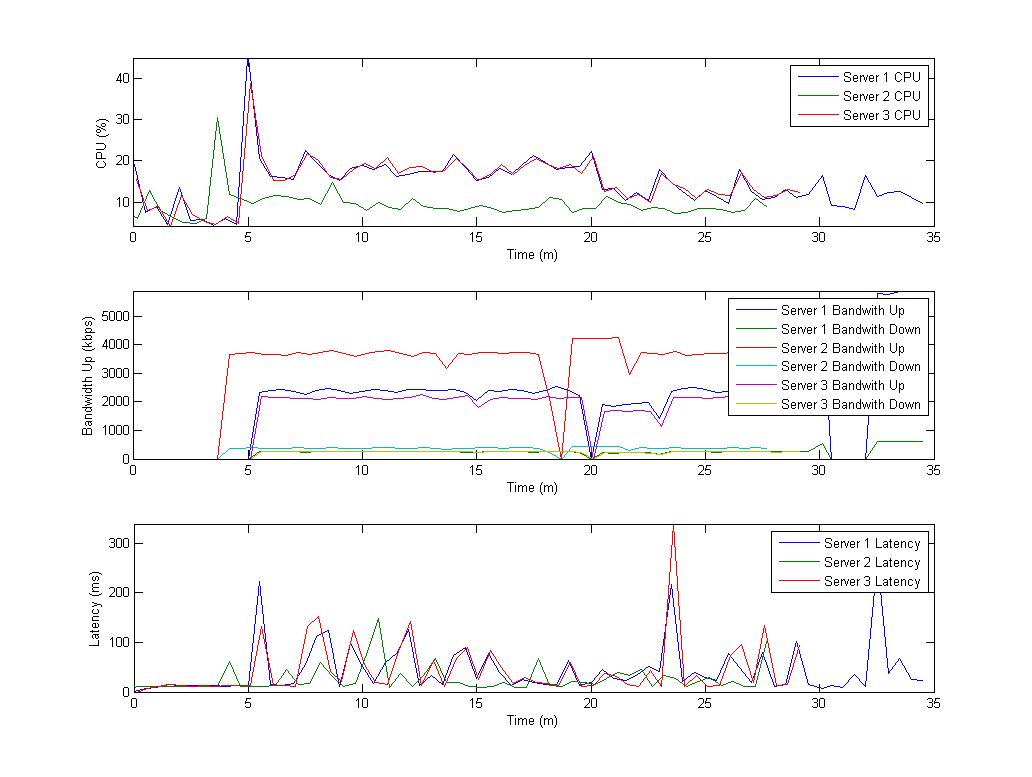
\includegraphics[width=0.75\columnwidth]{results/Run-3-lowmed/perf-1.png}
	\caption{Medium/low loaded cloud - Server performance}
	\label{fig:3serv-perf-lowmed}
\end{figure}

\subsubsection{Medium loaded cloud}

In the well balanced cloud case, one of the servers has less load than the other two servers and as such it has less bandwidth used when compared to the other two servers as seen in figure \ref{fig:3serv-perf-lowmed} - server 3 has less load. Because of this the pheromone at server 3 increases while the pheromone at the other two servers decreases. However, the average pheromone level across the cloud as seen by the ants is always bellow the thresholds and no house hunting optimization is triggered.

\begin{figure}
	\centering
		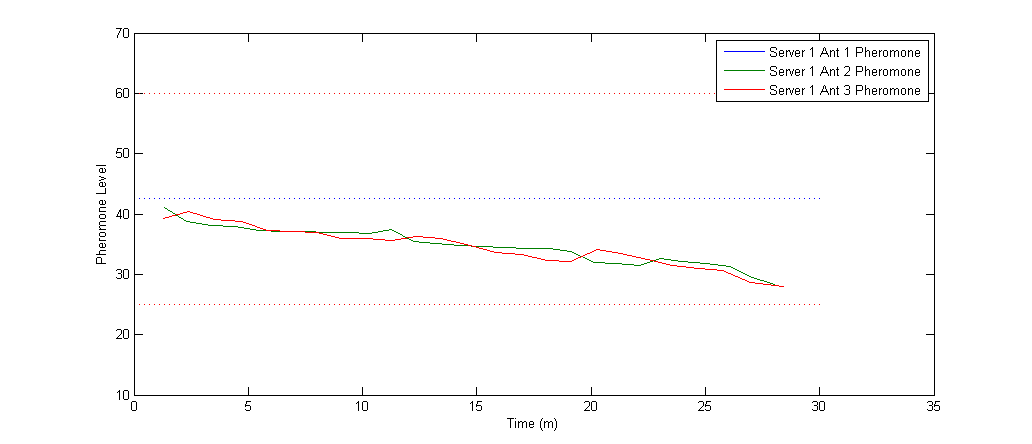
\includegraphics[width=0.75\columnwidth]{results/Run-3-med/ant-1.png}
	\caption{Medium loaded cloud - Pheromone at Server 1 as seen by ants}
	\label{fig:3serv-ant1-med}
\end{figure}

\begin{figure}
	\centering
		\includegraphics[width=0.75\columnwidth]{results/Run-3-med/ant-4.png}
	\caption{Medium loaded cloud - Pheromone at Server 2 as seen by ants}
	\label{fig:3serv-ant4-med}
\end{figure}

\begin{figure}
	\centering
		\includegraphics[width=0.75\columnwidth]{results/Run-3-med/ant-7.png}
	\caption{Medium loaded cloud - Pheromone at Server 3 as seen by ants}
	\label{fig:3serv-ant7-med}
\end{figure}

\begin{figure}
	\centering
		\includegraphics[width=0.75\columnwidth]{results/Run-3-med/server-1.png}
	\caption{Medium loaded cloud - Pheromone as seen by servers}
	\label{fig:3serv-pher-med}
\end{figure}

\begin{figure}
	\centering
		\includegraphics[width=0.75\columnwidth]{results/Run-3-med/perf-1.png}
	\caption{Medium loaded cloud - Server performance}
	\label{fig:3serv-perf-med}
\end{figure}

\subsubsection{Medium/high loaded cloud}

This test case tests a cloud which is slightly overloaded. The three servers are insufficient to meet the demands of the clients but barely, as can be seen in figure \ref{fig:3serv-perf-medhigh} where the CPU usage, bandwidth and latency show that more servers are needed to serve clients in the cloud. After approximately 12 minutes an SLA breach is detected and the house hunting optimization algorithm runs and decides to add 2 more servers to the cloud. After the two new servers are added one of the servers is underloaded, two of the servers are properly loaded and two of the servers are overloaded, as seen in figure \ref{fig:3serv-pher-medhigh} where after 15 minutes Server 2 and Server 5 maintain good pheromone levels, Server 1 has increasing pheromone levels (thus being underloaded) while servers 3 and 4 have decreasing pheromones being overloaded. This can also be seen in figure \ref{fig:3serv-perf-medhigh} looking at the bandwidth up graphs, where server 1 has very low bandwidth used, servers 3 and 4 have high bandwidth and servers 2 and 5 have medium bandwidth used.

\begin{figure}
	\centering
		\includegraphics[width=0.75\columnwidth]{results/Run-3-medhigh/ant-1.png}
	\caption{Medium/high loaded cloud - Pheromone at Server 1 as seen by ants}
	\label{fig:3serv-ant1-medhigh}
\end{figure}

\begin{figure}
	\centering
		\includegraphics[width=0.75\columnwidth]{results/Run-3-medhigh/ant-6.png}
	\caption{Medium/high loaded cloud - Pheromone at Server 2 as seen by ants}
	\label{fig:3serv-ant6-medhigh}
\end{figure}

\begin{figure}
	\centering
		\includegraphics[width=0.75\columnwidth]{results/Run-3-medhigh/ant-11.png}
	\caption{Medium/high loaded cloud - Pheromone at Server 3 as seen by ants}
	\label{fig:3serv-ant11-medhigh}
\end{figure}

\begin{figure}
	\centering
		\includegraphics[width=0.75\columnwidth]{results/Run-3-medhigh/ant-16.png}
	\caption{Medium/high loaded cloud - Pheromone at Server 4 as seen by ants}
	\label{fig:3serv-ant16-medhigh}
\end{figure}

\begin{figure}
	\centering
		\includegraphics[width=0.75\columnwidth]{results/Run-3-medhigh/ant-21.png}
	\caption{Medium/high loaded cloud - Pheromone at Server 5 as seen by ants}
	\label{fig:3serv-ant25-medhigh}
\end{figure}

\begin{figure}
	\centering
		\includegraphics[width=0.75\columnwidth]{results/Run-3-medhigh/server-1.png}
	\caption{Medium/high loaded cloud - Pheromone as seen by servers}
	\label{fig:3serv-pher-medhigh}
\end{figure}

\begin{figure}
	\centering
		\includegraphics[width=0.75\columnwidth]{results/Run-3-medhigh/perf-1.png}
	\caption{Medium/high loaded cloud - Server performance}
	\label{fig:3serv-perf-medhigh}
\end{figure}

\subsubsection{Over loaded/under loaded cloud}

In this case the cloud is first over loaded and then suddenly the streaming clients stop and the cloud becomes underloaded. In the first part of the test the three servers are insufficient to meet the demands of the clients as seen in the performance graphs with high bandwidth, latency and CPU usage. This causes the pheromone in the cloud to drop until a SLA breach is detected and new servers are added to the cloud. The pheromone drop is faster than in the previous case due to more load on the server. After new servers are added to the cloud the performance improves as seen by lower bandwidth at each servers, and this remains stable until users stop streaming, at which point the usage drops and the pheromone increases until a new SLA breach is detected and three servers are removed.

The first SLA breach results in two servers being added to the cloud. This is because of the fact that all three ants' initial solution starts with adding 2 new servers. The second SLA breach is more interesting however:

\begin{enumerate}
	\item Initial solutions: 
	\begin{itemize}
		\item Ant 1 goes to Nest 1 - remove three servers
		\item Ant 2 goes to Nest 2 - remove two servers
		\item Ant 3 goes to Nest 3 - remove four server
		\item Ant 4 goes to Nest 4 - remove three server
		\item Ant 5 goes to Nest 5 - remove three server
	\end{itemize}
	\item Recruitment:
	\begin{itemize}
		\item Ant 1 recruits Ant 4 and nest 4 is dropped out as no ants go to it
		\item Ant 5 recruits Ant 3 and nest 3 is dropped out as no ants go to it
		\item Ant 2 recruits a newly created ant which looks like Ant 2
	\end{itemize}
	\item Recruitment:
	\begin{itemize}
		\item Ant 1 recruits Ant 5 and Ant 4 recruits ant 3, nest 5 is dropped out
	\end{itemize}
	\item Recruitment:
	\begin{itemize}
		\item Ant 1 recruits Ant 2
	\end{itemize}
	\item All ants go to same solution which is nest 1
\end{enumerate}

\begin{figure}
	\centering
		\includegraphics[width=0.75\columnwidth]{results/Run-3-high/ant-1.png}
	\caption{Over loaded cloud - Pheromone at Server 1 as seen by ants}
	\label{fig:3serv-ant1-high}
\end{figure}

\begin{figure}
	\centering
		\includegraphics[width=0.75\columnwidth]{results/Run-3-high/ant-6.png}
	\caption{Over loaded cloud - Pheromone at Server 2 as seen by ants}
	\label{fig:3serv-ant6-high}
\end{figure}

\begin{figure}
	\centering
		\includegraphics[width=0.75\columnwidth]{results/Run-3-high/ant-11.png}
	\caption{Over loaded cloud - Pheromone at Server 3 as seen by ants}
	\label{fig:3serv-ant11-high}
\end{figure}

\begin{figure}
	\centering
		\includegraphics[width=0.75\columnwidth]{results/Run-3-high/ant-16.png}
	\caption{Over loaded cloud - Pheromone at Server 4 as seen by ants}
	\label{fig:3serv-ant16-high}
\end{figure}

\begin{figure}
	\centering
		\includegraphics[width=0.75\columnwidth]{results/Run-3-high/ant-21.png}
	\caption{Over loaded cloud - Pheromone at Server 5 as seen by ants}
	\label{fig:3serv-ant21-high}
\end{figure}

\begin{figure}
	\centering
		\includegraphics[width=0.75\columnwidth]{results/Run-3-high/server-1.png}
	\caption{Over loaded cloud - Pheromone as seen by servers}
	\label{fig:3serv-pher-high}
\end{figure}

\begin{figure}
	\centering
		\includegraphics[width=0.75\columnwidth]{results/Run-3-high/perf-1.png}
	\caption{Over loaded cloud - Server performance}
	\label{fig:3serv-perf-high}
\end{figure}

\section{Simulation Autonomic Computing Performance Tests}

The second set of tests for the performance of the self-organizing system presented in this thesis were run on top of the simulation environment presented in the previous chapter. A number of tests were run, with different workloads in order to determine the performance of the system and also compare how the developed ant based system performs compare to other auto scaling systems. Due to the fact that the workloads are generated stochastically, each of the tests was run 5 times and the results were aggregated. The performance tests only focus on the auto-scaling algorithm for the application tier and assume that the cloud has enough hosts and also that the cloud has enough database VMs to take care of the load. For this purpose all simulations are run with 60 host computers which can run VMs and 30 database VMs which are always up. Each of the hosts is defined as having 2 CPU cores, each of which provides 1000 MIPS. All of the application VMs are equal in power and they provide 250 MIPS to the simulated web application running on top of the VM. Each of the simulations is run for 48 hours, with a workload defined for 24 hours and which repeats after the first 24 hours. Workloads are generated using a Gaussian distribution.

\subsection{Low workload, low number of VMs}

The first simulation run is a simulation where the workload is low and as such not a large number of VMs are required to run at the same time in order to meet the desired SLAs for the application.

The workload for this test starts with a mean of 60 sessions per hour and a standard deviation of 1 and gradually increases towards a mean of 1000 sessions per hour with a standard deviation of 5, at 10 - 12 hours. This is followed by a small drop at 13 hours to 500 sessions after which the load goes back to 1000 sessions for hour until 17 hours. After this, the workload decreases gradually until it reaches 30 sessions per hour with a standard deviation of 1 at 24 hours. The distribution of the sessions per hour can be seen in Figure \ref{fig:sim1-workload}.

\begin{figure}
	\centering
		\includegraphics[width=0.75\columnwidth]{results/sim1/sim1-workload.png}
	\caption{Simulation - low workload}
	\label{fig:sim1-workload}
\end{figure}

Figures \ref{fig:sim1-basestats}, \ref{fig:sim1-antSimplestats} and \ref{fig:sim1-antHHstats} show the statistical results for the simulation runs. The results are averaged per hour and across the 5 runs for each auto-scaling algorithm. The graphs include average CPU usage as well as average number of sessions per server and average provisioned servers. Looking at the three graphs, it can be seen that the simple ant auto scaling algorithm obtains better CPU utilization than the simple auto scaling approach, and better than the house hunting algorithm also. At the same time, the simple ant auto scaling algorithm achieves this, while maintaining the server count more stable than the simple auto scaling algorithm.

\begin{figure}
	\centering
		\includegraphics[width=0.75\columnwidth]{results/sim1/sim1-basestats.png}
	\caption{Simulation - Simple autoscaling}
	\label{fig:sim1-basestats}
\end{figure}

\begin{figure}
	\centering
		\includegraphics[width=0.75\columnwidth]{results/sim1/sim1-antSimplestats.png}
	\caption{Simulation - Simple ant autoscaling}
	\label{fig:sim1-antSimplestats}
\end{figure}

\begin{figure}
	\centering
		\includegraphics[width=0.75\columnwidth]{results/sim1/sim1-antHHstats.png}
	\caption{Simulation - House hunting ant autoscaling}
	\label{fig:sim1-antHHstats}
\end{figure}

Similar results can be seen in Table \ref{table:sim1} which summarizes the tests. The simple scaling algorithm takes a lot more scale up and scale down actions than the two ant based algorithms. This is because as soon as the average utilization breaches the thresholds an action must be taken, while for the ant algorithms the detection is not triggered by a single drop or spike in utilization. At the same time, the simple ant scaling algorithm has a much shorter time when the cloud is over provisioned (too many servers for the load) compared to the simple scaling algorithm, and longer periods when the cloud is under high usage with over 90\% and 95\% CPU usage. The house hunting algorithm performs worse than the simple ant algorithm for this test, as it tends to over provision the cloud when a breach is predicted by adding too many servers. This can be seen, as it has higher scale up/down counts and also higher over provisioned times.

\begin{table}
\caption{Low workload simulation results}
\label{table:sim1}
\begin{tabu} to\linewidth{|X[c]|X[c]|X[c]|X[c]|X[c]|X[c]|X[c]|X[c]|}
\everyrow{\hline}
\hline
Scaling Algorithm & Scale Up Count & Scale Down Count & Over Provisioned - 10\% (s) & Over Provisioned - 20\% (s) & High usage - 95\% (s) & High usage - 90\% (s) \\
\taburowcolors 2{Gray!20..LimeGreen!50}
Simple scaling & 755 & 762 & 12 & 163 & 3 & 8 \\
Simple ant scaling & 128 & 132 & 9 & 53 & 50 & 79 \\
House hunting scaling & 223 & 339 & 101 & 377 & 37 & 64 \\
\end{tabu}
\end{table}

\section{Self-organizing self-optimization test conclusions}

The performance tests show that the system behaves as desired and that the ACO algorithm properly detects a breach of SLA when the cloud is under loaded or over loaded while the house hunting algorithm can determine the number of servers added or removed. Due to the randomness which exists inside the house hunting algorithm it is possible to overshoot or undershoot the correct number of servers, however this is corrected quickly after another SLA breach is detected.


\chapter{Conclusions} % Write in your own chapter title
\label{Chapter_conclusion}
\lhead{Chapter \ref{Chapter_conclusion}. \emph{Conclusions}} % Write in your own chapter title to set the page header

This thesis has presented a self-organizing, autonomic system responsible for managing cloud resources. The thesis has presented two algorithms for such a self-organizing system - one to detect the SLA breach and one to optimize the number of servers in the cloud. A test bed and a simulation were also created to run the application and validate the control system. Results were obtained, which prove that the control of the system can not be achieved by simply managing the CPU usage of the servers and that a more complex system, like the one presented in the thesis has to be used.

The novelty of the thesis comes from two separate parts which support each other:

\begin{enumerate}
	\item The ACO algorithm used in order to detect breaches of SLA. Normally the ACO is used in order to optimize the solution of a problem, however the thesis uses a modified version of the ACO in order to analyze the behaviour of the cloud, predict breaches of SLA and take corrective measures.
	\item A new self-organizing algorithm based on the behaviour of ants while house hunting is implemented and experiments to validate it are introduced. The algorithm is inspired by prior work and modeling into the behaviour of ants while house hunting, however there is no known algorithm which implements the behaviour in order to optimize a given problem.
\end{enumerate}

The thesis opens a number of avenues for future work and improvements to the new algorithms introduced:

\begin{enumerate}
	\item The house hunting algorithm can be improved to take in consideration the fitness of a solution when recruiting. While the fitness should not be the only factor in deciding which ant should recruit another, it can be used to bias positively solutions with better fitness. The current solution uses the fitness only to remove solutions with very poor fitness from the solution set.
	\item Further tests and simulations can be run on the created infrastructure in order to use more complex workloads and determine the behaviour of the proposed systems.
\end{enumerate}
 % Results

%\input{./Chapters/Chapter6} %  Conclusion

%\input{./Chapters/Chapter7} %  Conclusion

%\input{./Chapters/Chapter8} %  Conclusion

%\input{./Chapters/Chapter9} %  Conclusion

%% ----------------------------------------------------------------
% Now begin the Appendices, including them as separate files

\addtocontents{toc}{\vspace{2em}} % Add a gap in the Contents, for aesthetics

% \appendix % Cue to tell LaTeX that the following 'chapters' are Appendices

% \input{./Appendices/Appendix_Model}	% Appendix Title

% \input{./Appendices/Appendix_Cloud_Measure_Multi} % Appendix Title

%\input{./Appendices/AppendixC} % Appendix Title

% \addtocontents{toc}{\vspace{2em}}  % Add a gap in the Contents, for aesthetics
\backmatter

%% ----------------------------------------------------------------
\label{Bibliography}
\lhead{\emph{Bibliography}}  % Change the left side page header to "Bibliography"
\bibliographystyle{IEEEtran}  % Use the "unsrtnat" BibTeX style for formatting the Bibliography, amsplain would do it by author name
\bibliography{Resources/Bibliography/Bibliography}  % The references (bibliography) information are stored in the file named "Bibliography.bib"

\end{document}  % The End
%% ----------------------------------------------------------------